% !TEX TS-program = pdflatexmk
\documentclass[tikz]{article}
% Compiles in TeXShop 5.54 using pdflatexmk. 

%\usepackage[utf8x]{inputenc}  % Support unicode characters
%	\DeclareUnicodeCharacter{2316}{\positionIndicator}
%%	\DeclareUnicodeCharacter{2316}{⌖}
%\usepackage{newunicodechar}
%\newunicodechar{⌖}{\positionIndicator}

%% Use sans-serif fonts:
%\renewcommand{\familydefault}{\sfdefault}

% Make document be in landscape orientation
\usepackage[letterpaper,portrait,margin=0.0cm]{geometry}
\usepackage{multicol}
\usepackage[dvipsnames]{xcolor}

\usepackage{gensymb}  % for \degree

\usepackage{tikz}
\usetikzlibrary{calc}  
%\usetikzlibrary{calendar}  % For lunar phases, per https://tex.stackexchange.com/a/34805/25653
%\usetikzlibrary{fpu}  % For lunar phases, per https://tex.stackexchange.com/a/34805/25653
\usetikzlibrary{decorations.text}

\usepackage{hyperref}   % should be last!
\hypersetup{
    bookmarks=false,         % show bookmarks bar?
    unicode=false,          % non-Latin characters in Acrobat's bookmarks
    pdftoolbar=false,        % show Acrobat's toolbar?
    pdfmenubar=false,        % show Acrobat's menu?
    pdffitwindow=true,     % window fit to page when opened
    pdfstartview={FitH},    % fits the width of the page to the window
    pdftitle={Solar Motion Simulator},    % title
    pdfauthor={Jess W Vriesema},     % author
    pdfsubject={Solar Motion Simulator},   % subject of the document
    pdfcreator={Jess W Vriesema},   % creator of the document
    pdfproducer={Jess W Vriesema}, % producer of the document
    pdfkeywords={Earth}{Sun}{Simulation}{Astronomy}{Solar Motion}{Horizon}{Printable} % list of keywords
    pdfnewwindow=true,      % links in new window
    colorlinks=true,       % false: boxed links; true: colored links
%    linkcolor=[rgb]{0.2,0.2,0.95},          % color of internal links
%    citecolor=blue,        % color of links to bibliography
%    filecolor=magenta,      % color of file links
    urlcolor=blue           % color of external links
}






% ------------------------------------------------------------------------- %
% DOCUMENT SETTINGS (switches)
% ------------------------------------------------------------------------- %
% See https://ramblingacademic.com/2016/10/31/multiple-latex-document-versions/ for examples
% Declare new switches (default value of false)
\newif\ifPrintHelperLines  % if true, print "helper lines" (1cm x 1cm grid) -- not recommended
%\PrintHelperLinestrue  % set \printHelperLines to true

\newif\ifPrintInstructions  % if true, print page of instructions
\PrintInstructionsfalse  % set \PrintInstructions to false

\newif\ifLaserCutterMode  % if true, color laser-cutter lines a special color
%\LaserCutterModetrue  % set \LaserCutterMode to true
\LaserCutterModefalse  % set \LaserCutterMode to false
\newcommand*{\LaserCutterKerf}{0.04cm}  % width of the laser beam's cut

\newif\ifLaserCutFolds  % if true, use laser-cutter to perforate folds (ignored if \LaserCutterMode is false)
\LaserCutFoldstrue  % set \LaserCutFolds to true
\newcommand*{\LaserCutFoldWidth}{0.2cm}  % extra space at edges for fold

\newif\ifUseHDTeeth  % if true, use laser-cutter to create "teeth" along the Horizon Disk incision instead of a line
\UseHDTeethtrue % set \UseHDTeeth to true


\newif\ifPrintWishlist  % if true, print page of wishlist (for developer's use only.)
%\PrintWishlisttrue  % set \PrintWishlist to true




% To see where the nullfont errors are:
%\font\nullfont=cmr10
% Possibly because I have circle(\someRadius); vs. circle[radius=\someRadius];?
%\tracinglostchars=2
%\tracingmacros=1  % BAD -- I cut the process after it created A 1.46 GB logfile. 


% ------------------------------------------------------------------------- %
% MACRO DEFINITIONS
% ------------------------------------------------------------------------- %

\newcommand*{\mountainFold}{dashed}
\newcommand*{\valleyFold}{dotted}
\newcommand*{\mountainAndValleyFold}{dash dot}

% Registration Mark  -- based on https://tex.stackexchange.com/a/471576/25653
%\newcommand{\regMark}{(0,0) -- (2,0) (1,1) -- (1,-1) (.5,0) arc (0:360:-.5)}


%\definecolor(5,85,5,0){hotPink}  % not colorblind-safe
%\definecolor(60,10,100,0){dullGreen}  % not colorblind-safe
\definecolor{kellyGreen}{RGB}{27,158,119}
\definecolor{burntOrange}{RGB}{217,95,2}
\definecolor{lavendar}{RGB}{117,112,179}
\definecolor{light-gray}{gray}{0.75}



% Line Widths
\newcommand*{\OutlineWidth}{2pt}
\newcommand*{\IncisionWidth}{2.5pt}
\newcommand*{\LaserCutterLineWidth}{\LaserCutterKerf}
\newcommand*{\LaserCutterHalfTieWidth}{2*\LaserCutterKerf} % Half the width of a "tie" (paper/joiner part in a dashed cut)

% Line Colors
\newcommand*{\FillColor}{gray!20}
\newcommand*{\OutlineColor}{black}
\newcommand*{\IncisionColor}{blue}
\newcommand*{\LaserCutterColor}{red}

% Laser cutter styles
\tikzset{LaserCutterFoldAid/.style=          {dash pattern=on 1pt off 4 pt}}%
%\tikzset{LaserCutterMostlyCut/.style=          {dash pattern=on 10pt off 1 pt}}%
\tikzset{LaserCutterOutlineCut/.style=          {dash pattern=on 20pt off 1 pt}}%
\tikzset{LaserCutterCut/.style=          {dash pattern=}}%



% ------------------------------------------------------------------------- %
% SHAPE SETTINGS
% ------------------------------------------------------------------------- %
\newcommand*{\axialTilt}{23.5}  % Earth's tilt, in degrees
%\newcommand*{\axialTilt}{23.44}  % Earth's tilt, in degrees



% Page Positioning
\newcommand*{\masterXShift}{0cm}
\newcommand*{\masterYShift}{0cm}
%\newcommand*{\masterXShift}{1.73cm}
%\newcommand*{\masterYShift}{-10.9cm}

\newcommand*{\FoldKeyXShift}{5.5cm+\masterXShift}
\newcommand*{\FoldKeyYShift}{8cm+\masterYShift}
\newcommand*{\FoldKeyRotation}{0}

%\newcommand*{\QRXShift}{6cm+\masterXShift}
%\newcommand*{\QRYShift}{8cm+\masterYShift}
%\newcommand*{\QRRotation}{0}

\newcommand*{\RegMarkUpperLeftXShift}{-11.5cm+\masterXShift}
\newcommand*{\RegMarkUpperLeftYShift}{10.5cm+\masterYShift}
\newcommand*{\RegMarkLowerRightXShift}{8cm+\masterXShift}
\newcommand*{\RegMarkLowerRightYShift}{-15.42cm+\masterYShift}

%\newcommand*{\RegMarkLowerLeftXShift}{-11.5cm+\masterXShift}
%\newcommand*{\RegMarkLowerLeftYShift}{-15.42cm+\masterYShift}
%\newcommand*{\RegMarkUpperRightXShift}{10.5cm+\masterXShift}
%\newcommand*{\RegMarkUpperRightYShift}{8cm+\masterYShift}

\newcommand*{\RegMarkAXShift}{6.5cm+\masterXShift}
\newcommand*{\RegMarkAYShift}{-14cm+\masterYShift}
%\newcommand*{\RegMarkAXShift}{-0.5cm+\masterXShift}  % bottom center, next to instruction box
%\newcommand*{\RegMarkAYShift}{-14cm+\masterYShift}
\newcommand*{\RegMarkBXShift}{-10cm+\masterXShift}
\newcommand*{\RegMarkBYShift}{9cm+\masterYShift}
%\newcommand*{\RegMarkBXShift}{-5cm+\masterXShift}  % in the solar frame cavity
%\newcommand*{\RegMarkBYShift}{7cm+\masterYShift}

\newcommand*{\HelpCardXShift}{-6.35cm+\masterXShift}
\newcommand*{\HelpCardYShift}{-11.5cm+\masterYShift}
\newcommand*{\HelpCardRotation}{0}

%\newcommand*{\HelpCardXShift}{-6.5cm+\masterXShift}
%\newcommand*{\HelpCardYShift}{-11.5cm+\masterYShift}
%\newcommand*{\HelpCardRotation}{0}

\newcommand*{\HorizonDiskXShift}{3.5cm+\masterXShift}
\newcommand*{\HorizonDiskYShift}{-9.75cm+\masterYShift}
\newcommand*{\HorizonDiskRotation}{0}

%\newcommand*{\HorizonDiskXShift}{3cm+\masterXShift}
%\newcommand*{\HorizonDiskYShift}{-10cm+\masterYShift}
%\newcommand*{\HorizonDiskRotation}{0}

\newcommand*{\TimeDiskXShift}{5.05cm+\masterXShift}
\newcommand*{\TimeDiskYShift}{-1.9cm+\masterYShift}
\newcommand*{\TimeDiskRotation}{0}

%\newcommand*{\TimeDiskXShift}{4cm+\masterXShift}
%\newcommand*{\TimeDiskYShift}{-2cm+\masterYShift}
%\newcommand*{\TimeDiskRotation}{0}

\newcommand*{\SunCarriageXShift}{6cm+\masterXShift}
\newcommand*{\SunCarriageYShift}{2.625cm+\masterYShift}
\newcommand*{\SunCarriageRotation}{0}

%\newcommand*{\SunCarriageXShift}{-9cm+\masterXShift}
%\newcommand*{\SunCarriageYShift}{-5.5cm+\masterYShift}
%\newcommand*{\SunCarriageRotation}{90}

\newcommand*{\SolarFrameXShift}{-3cm+\masterXShift}
\newcommand*{\SolarFrameYShift}{4cm+\masterYShift}
\newcommand*{\SolarFrameRotation}{0}

%\newcommand*{\SolarFrameXShift}{-5cm+\masterXShift}
%\newcommand*{\SolarFrameYShift}{4cm+\masterYShift}
%\newcommand*{\SolarFrameRotation}{0}

\newcommand*{\SolarFrameFootXShift}{-8.9cm+\masterXShift}
\newcommand*{\SolarFrameFootYShift}{-4.5cm+\masterYShift}
\newcommand*{\SolarFrameFootRotation}{0}

%\newcommand*{\SolarFrameFootXShift}{4.5cm+\masterXShift}
%\newcommand*{\SolarFrameFootYShift}{6cm+\masterYShift}
%\newcommand*{\SolarFrameFootRotation}{0}

\newcommand*{\LastUpdateMsgXShift}{3.5cm+\masterXShift}
\newcommand*{\LastUpdateMsgYShift}{-14.9cm+\masterYShift}
\newcommand*{\LastUpdateMsgRotation}{0}


% Registration Marks (circle and crosshairs)
\newcommand*{\RegMarkScale}{0.5cm}
\newcommand*{\RegMarkCornerLineWidth}{1pt}
\newcommand*{\RegMarkCornerLength}{2cm}
\newcommand*{\RegMarkCornerMargin}{1cm}
\newcommand*{\RegMarkLineStyle}{solid}
% Corner Alignment Marks (diagonal line and L-shape)
\newcommand*{\RegMarkSmallLineScale}{0.3cm}
\newcommand*{\RegMarkDiagonalLineStyle}{solid}



% Folding Key — inspired by https://www.cutoutfoldup.com/1804-key-to-symbols-in-fold-diagrams.php.
\newcommand*{\FoldKeyScale}{1cm}
\newcommand*{\FoldKeyLineWidth}{1pt}
\newcommand*{\FoldKeyLengthA}{1.5cm}  % slightly down and more to the right
\newcommand*{\FoldKeyLengthB}{2.5cm}  % up and to the right
\newcommand*{\FoldKeyLengthC}{1.5cm}  % more down and slightly to the right
\newcommand*{\FoldKeyAngleA}{-15}  % slightly down and more to the right
\newcommand*{\FoldKeyAngleB}{45}  % up and to the right
\newcommand*{\FoldKeyAngleC}{-60}  % more down and slightly to the right
\newcommand*{\FoldKeyTextScale}{0.9}


% Help Card
\newcommand*{\HelpCardBorderWidth}{\OutlineWidth}
\newcommand*{\HelpCardHeight}{7cm}
\newcommand*{\HelpCardWidth}{9.5cm}
\newcommand*{\HelpDiskTextScale}{0.72}
\newcommand*{\HelpDiskTextMargin}{0.25cm}



% Time Disk
\newcommand*{\TimeDiskRadius}{3cm}
\newcommand*{\TimeDiskIncisionExtraSize}{0.0cm}
%\newcommand*{\TimeDiskIncisionSize}{\TimeDiskRadius+\TimeDiskIncisionExtraSize}
\newcommand*{\TimeDiskIncisionWidth}{\IncisionWidth}

\newcommand*{\TimeDiskUndersideAlignmentLineWidth}{0.03cm}

\newcommand*{\TimeDiskCardinalHourTickSize}{0.5cm}
\newcommand*{\TimeDiskCardinalHourTickWidth}{0.07cm}
\newcommand*{\TimeDiskCardinalHourLabelOffset}{0.15cm}
\newcommand*{\TimeDiskCardinalHourLabelScale}{1.3}

\newcommand*{\TimeDiskHourTickSize}{0.3cm}
\newcommand*{\TimeDiskHourTickWidth}{0.03cm}
\newcommand*{\TimeDiskHourLabelOffset}{0.1cm}
\newcommand*{\TimeDiskHourLabelScale}{0.85}

\newcommand*{\TimeDiskHalfHourTickSize}{0.2cm}
\newcommand*{\TimeDiskHalfHourTickWidth}{0.01cm}

\newcommand*{\TimeDiskQuarterHourTickSize}{0.1cm}
\newcommand*{\TimeDiskQuarterHourTickWidth}{0.01cm}

\newcommand*{\TimeDiskLabelScale}{1.5}
\newcommand*{\TimeDiskLabelRadius}{0.30*\TimeDiskRadius}



% Sun Carriange
%\newcommand*{\SunCarriageWidth}{{{1.5*\SolarFrameOuterRadius}-{1.5*\SolarFrameInnerRadius}}}
\newcommand*{\SunCarriageWidth}{1.8cm}
\newcommand*{\SunCarriageHeight}{\SunCarriageWidth}
\newcommand*{\SunCarriageInternalWidth}{0.4cm}
\newcommand*{\SunCarriageIndicatorSize}{0.2cm}
\newcommand*{\SunCarriageFlapWidth}{0.3cm} % Slightly more than \SunCarriageInternalWidth/2
\newcommand*{\SunCarriageInternalCircleRadii}{0.30cm} % US standard diameter is 1/4"–5/16 in (6-8mm)
\newcommand*{\SunCarriageInternalCircleCrosshairs}{0.3*\SunCarriageInternalCircleRadii} 
\newcommand*{\SunCarriageInternalCircleLineStyle}{}
\newcommand*{\SunCarriageInternalCircleLineWidth}{0.5pt}

\newcommand*{\drawHolePunch}[2]{
	% #1: x
	% #2: y
	% Draw circle
	\draw[\SunCarriageInternalCircleLineStyle,line width=\SunCarriageInternalCircleLineWidth] (#1,#2) circle (\SunCarriageInternalCircleRadii);
	% Draw crosshairs
	\draw[line width=\SunCarriageInternalCircleLineWidth] (#1-\SunCarriageInternalCircleCrosshairs,#2) -- (#1+\SunCarriageInternalCircleCrosshairs,#2);
	\draw[line width=\SunCarriageInternalCircleLineWidth] (#1,#2-\SunCarriageInternalCircleCrosshairs) -- (#1,#2+\SunCarriageInternalCircleCrosshairs);
}



% Solar Frame
\newcommand*{\SolarFrameInnerRadius}{4.5cm}
\newcommand*{\SolarFrameOuterRadius}{6.0cm}
\newcommand*{\SolarFrameCenterSupportFlapLength}{2.5cm} % both right and left of (0,0)
\newcommand*{\SolarFrameCenterSupportFlapWidth}{1.25cm}
\newcommand*{\SolarFrameCenterLatitudeArcRadius}{3cm}

\newcommand*{\SolarFrameDeclinationMajorLineWidth}{0.05cm}
\newcommand*{\SolarFrameDeclinationMajorLineLength}{0.45cm}
\newcommand*{\SolarFrameDeclinationMajorLineLabelOffset}{0.35cm}
\newcommand*{\SolarFrameDeclinationMajorLineLabelScale}{0.7}

\newcommand*{\SolarFrameDeclinationMedLineWidth}{0.03cm}
\newcommand*{\SolarFrameDeclinationMedLineLength}{0.43cm}
\newcommand*{\SolarFrameDeclinationMedLineLabelOffset}{0.3cm}
\newcommand*{\SolarFrameDeclinationMedLineLabelScale}{1.0}

\newcommand*{\SolarFrameDeclinationMinorLineWidth}{0.01cm}
\newcommand*{\SolarFrameDeclinationMinorLineLength}{0.35cm}
\newcommand*{\SolarFrameDeclinationMinorLineLabelOffset}{0.3cm}
\newcommand*{\SolarFrameDeclinationMinorLineLabelScale}{1.0}

\newcommand*{\SolarFrameDeclinationLabelRadius}{\SolarFrameOuterRadius-0.45cm}

\newcommand*{\SolarFrameLatitudeMajorLineWidth}{0.03cm}
\newcommand*{\SolarFrameLatitudeMajorLineLength}{0.3cm}
\newcommand*{\SolarFrameLatitudeMajorLineLabelOffset}{0.45cm}
\newcommand*{\SolarFrameLatitudeMajorLineLabelScale}{0.9}

\newcommand*{\SolarFrameLatitudeMinorLineWidth}{0.015cm}
\newcommand*{\SolarFrameLatitudeMinorLineLength}{0.2cm}

\newcommand*{\SolarFrameLatitudeLabelRadius}{\SolarFrameCenterLatitudeArcRadius+0.55cm}
\newcommand*{\SolarFrameTimeDiskIncisionWidth}{\IncisionWidth}
\newcommand*{\SolarFrameLabelOffset}{0.5cm}
\newcommand*{\SolarFrameLabelScale}{1.4}
\newcommand*{\SolarFrameTimeLabelScale}{1.0}
\newcommand*{\SolarFrameTimeLabelOffset}{0.3cm}
\newcommand*{\SolarFrameFootLabelScale}{1.0}
\newcommand*{\SolarFrameCopyrightLabelRadius}{\SolarFrameOuterRadius-0.25cm}



% Solar Frame Foot
\newcommand*{\SolarFrameFootLength}{0.8*\TimeDiskRadius}
\newcommand*{\SolarFrameFootHeight}{3cm}
\newcommand*{\SolarFrameExtraFootHeight}{1.0*\SolarFrameFootLength}
\newcommand*{\FooterSupportLabelOffset}{0.3cm}
\newcommand*{\FooterSupportLabelScale}{1.4}



% Horizon Disk
\newcommand*{\HorizonDiskRadius}{4cm}
\newcommand*{\HorizonDiskNinetyDegTickSize}{0.8cm}
\newcommand*{\HorizonDiskNinetyDegTickWidth}{0.05cm}
\newcommand*{\HorizonDiskNinetyDegLabelOffset}{0.35cm}
\newcommand*{\HorizonDiskNinetyDegLabelScale}{1.5}
\newcommand*{\HorizonDiskThirtyDegTickSize}{0.6cm}
\newcommand*{\HorizonDiskThirtyDegTickWidth}{0.02cm}
\newcommand*{\HorizonDiskThirtyDegLabelOffset}{0.25cm}
\newcommand*{\HorizonDiskThirtyDegLabelScale}{0.9}
\newcommand*{\HorizonDiskTenDegTickSize}{0.4cm}
\newcommand*{\HorizonDiskFiveDegTickSize}{0.3cm}
\newcommand*{\HorizonDiskOneDegTickSize}{0.2cm}
\newcommand*{\HorizonDiskLabelRadius}{0.30*\HorizonDiskRadius}
\newcommand*{\HorizonDiskLabelScale}{1.5}
\newcommand*{\HorizonDiskIncisionWidth}{\IncisionWidth}
\newcommand*{\HorizonDiskSolarFrameLineWidth}{\OutlineWidth}
\newcommand*{\HorizonDiskTapeMeScale}{0.8}

% Horizon Frame Teeth
\newcommand*{\HorizonDiskTeeth}{3} % How many teeth on each side (IGNORED if \UseHDTeeth is unset)
\newcommand*{\HorizonDiskTeethMinRadius}{0.5*\SolarFrameCenterLatitudeArcRadius} % Inner boundary of teeth
\newcommand*{\HorizonDiskTeethMaxRadius}{0.9*\SolarFrameCenterLatitudeArcRadius} % Outer boundary of teeth
\newcommand*{\HorizonDiskTeethLength}{0.15cm} % How long the teeth are past the center line
\newcommand*{\HorizonDiskTeethHeight}{{(\HorizonDiskTeethMaxRadius-\HorizonDiskTeethMinRadius)/(2*\HorizonDiskTeeth)}} % Outer boundary of teeth — shortcut, not a setting


% ------------------------------------------------------------------------- %
% Math shorthands
\pgfmathsetmacro\laserCutterSolarFrameSineAngleOpp{\SolarFrameFootLength+\OutlineWidth/2-\LaserCutterLineWidth/2}
\pgfmathsetmacro\laserCutterSolarFrameSineAngleHyp{\SolarFrameOuterRadius+\OutlineWidth/2-\LaserCutterLineWidth/2}
\pgfmathsetmacro\laserCutterSolarFrameSineAngle{\laserCutterSolarFrameSineAngleOpp/\laserCutterSolarFrameSineAngleHyp}

\pgfmathsetmacro\laserCutterSolarFrameInnerSineAngleOpp{\OutlineWidth/2-\LaserCutterLineWidth/2}
\pgfmathsetmacro\laserCutterSolarFrameInnerSineAngleHyp{\SolarFrameInnerRadius+\OutlineWidth/2-\LaserCutterLineWidth/2}
\pgfmathsetmacro\laserCutterSolarFrameInnerSineAngle{\laserCutterSolarFrameInnerSineAngleOpp/\laserCutterSolarFrameInnerSineAngleHyp}

\pgfmathsetmacro\laserCutterSolarFrameLatSineAngleOpp{\OutlineWidth/2-\LaserCutterLineWidth/2}
\pgfmathsetmacro\laserCutterSolarFrameLatSineAngleHyp{\SolarFrameCenterLatitudeArcRadius+\OutlineWidth/2-\LaserCutterLineWidth/2}
\pgfmathsetmacro\laserCutterSolarFrameLatSineAngle{\laserCutterSolarFrameLatSineAngleOpp/\laserCutterSolarFrameLatSineAngleHyp}


%	-- ({270-asin(\SolarFrameFootLength/\SolarFrameOuterRadius)}:\SolarFrameOuterRadius+\OutlineWidth/2-\LaserCutterLineWidth/2) arc[start angle={270-asin(\SolarFrameFootLength/\SolarFrameOuterRadius)},end angle={-90+asin(\SolarFrameFootLength/\SolarFrameOuterRadius)},radius=\SolarFrameOuterRadius]
















% ------------------------------------------------------------------------- %


\begin{document}
\noindent
{\centering
%\resizebox{!}{\textheight}{%
%\resizebox{\textwidth}{!}{%














%% ------------------------------------------------------------------------- %
%% Draw the PRINT GUIDES
%% ------------------------------------------------------------------------- %
%\begin{tikzpicture}[overlay]
%% Registration Marks
%%\begin{scope}[xshift=current page.west,yshift=\RegMarkAYShift,rotate=0]
%\begin{scope}[shift={([xshift=2cm,yshift=2cm]current page.south west)}]
%	\draw[\RegMarkLineStyle] (-2*\RegMarkScale,0) -- (2*\RegMarkScale,0);
%	\draw[\RegMarkLineStyle] (0,-2*\RegMarkScale) -- (0,2*\RegMarkScale);
%	\draw[\RegMarkLineStyle] (0,0) circle (\RegMarkScale);
%\end{scope}
%
%\end{tikzpicture}


%\begin{tikzpicture}[remember picture,overlay]
%  \node [xshift=1cm,yshift=1cm] at (current page.south west)
%        [text width=7cm,fill=red!20,rounded corners,above right]
%  {
%    This is an absolutely positioned text in the
%    lower left corner. No shipout-hackery is used.
%  };
%\end{tikzpicture}
%\begin{tikzpicture}[remember picture,overlay]
%\node [xshift=1cm,yshift=1cm] at (current page.south west)
%[text width=7cm,fill=red!20,rounded corners,above right]
%{
%This is an absolutely positioned text in the
%lower left corner. No shipout-hackery is used.
%}; 
%\end{tikzpicture} 



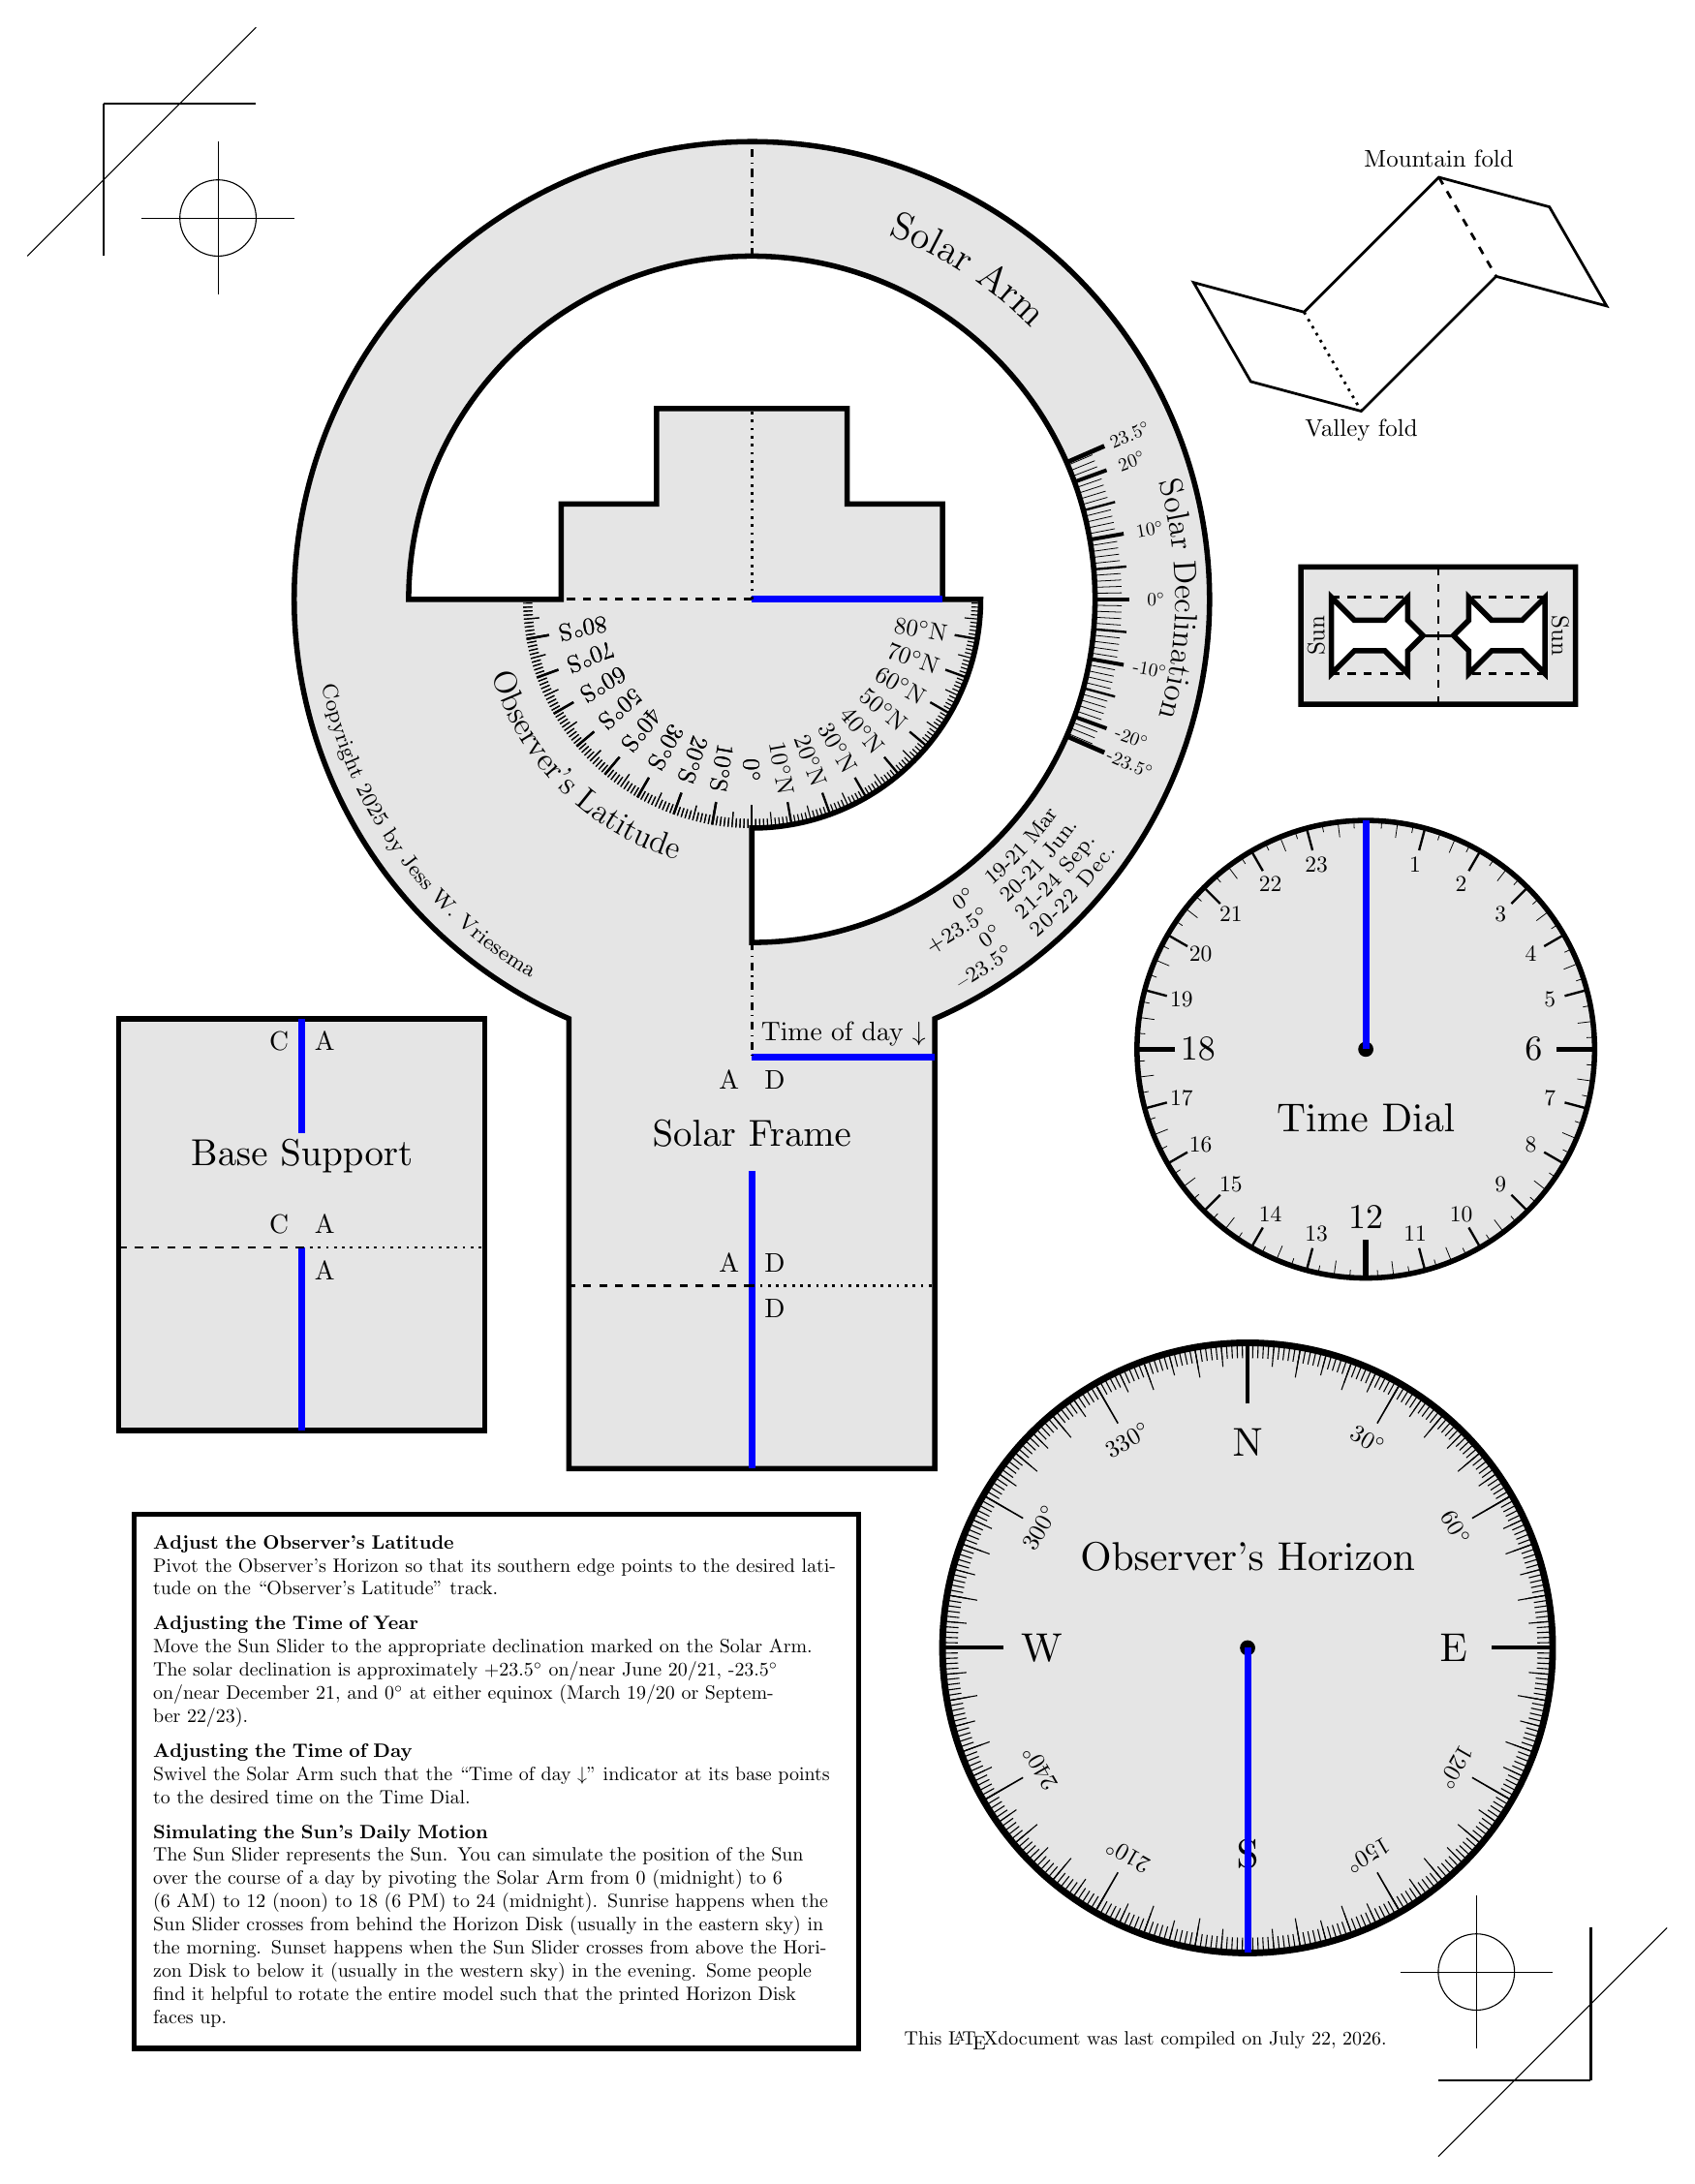
\begin{tikzpicture}%[overlay,remember picture]



% ------------------------------------------------------------------------- %
% Draw the PRINT GUIDES
% ------------------------------------------------------------------------- %

%% Registration Marks
%%\begin{scope}[xshift=current page.west,yshift=\RegMarkAYShift,rotate=0]
%\begin{scope}[shift={([xshift=1cm,yshift=1cm]current page.north west)}]
%	\draw[\RegMarkLineStyle] (-0.5cm,0) -- (0.5cm,0);
%	\draw[\RegMarkLineStyle] (0,-0.5cm) -- (0,0.5cm);
%	\draw[\RegMarkLineStyle] (0,0) circle (0.5cm);
%\end{scope}





%% ------------------------------------------------------------------------- %
%% Draw the QR CODE
%% ------------------------------------------------------------------------- %
%
%\begin{scope}[xshift=\QRXShift,yshift=\QRYShift,rotate=\QRRotation]
%
%	\node at (0,0) {\includegraphics[width=2.5cm]{qr_to_website.png}};
%
%\end{scope}







% ------------------------------------------------------------------------- %
% Draw the FOLD KEY
% ------------------------------------------------------------------------- %
\begin{scope}[xshift=\FoldKeyXShift,yshift=\FoldKeyYShift,rotate=\FoldKeyRotation]
	
	\ifLaserCutterMode
		 % Do nothing
	\else
		% Draw the Folding Key outline:
		\draw[line width=\FoldKeyLineWidth] (\FoldKeyAngleC:0.5*\FoldKeyLengthC) 
		-- ++(\FoldKeyAngleB:0.5*\FoldKeyLengthB)
		-- ++(\FoldKeyAngleA:\FoldKeyLengthA) 
		-- ++(\FoldKeyAngleC:-\FoldKeyLengthC) 
		-- ++(\FoldKeyAngleA:-\FoldKeyLengthA) 
		-- ++(\FoldKeyAngleB:-\FoldKeyLengthB) 
		-- ++(\FoldKeyAngleA:-\FoldKeyLengthA) 
		-- ++(\FoldKeyAngleC:\FoldKeyLengthC) 
		-- ++(\FoldKeyAngleA:\FoldKeyLengthA) -- cycle;
		
		% Draw the mountain fold indicator
		\draw[\mountainFold,line width=1pt]
			({0.5*\FoldKeyLengthB*cos(\FoldKeyAngleB)-0.5*\FoldKeyLengthC*cos(\FoldKeyAngleC)},{0.5*\FoldKeyLengthB*sin(\FoldKeyAngleB)-0.5*\FoldKeyLengthC*sin(\FoldKeyAngleC)}) 
			-- ({0.5*\FoldKeyLengthB*cos(\FoldKeyAngleB)+0.5*\FoldKeyLengthC*cos(\FoldKeyAngleC)},{0.5*\FoldKeyLengthB*sin(\FoldKeyAngleB)+0.5*\FoldKeyLengthC*sin(\FoldKeyAngleC)});
		% Draw the valley fold indicator
		\draw[\valleyFold,line width=1pt]
			({-0.5*\FoldKeyLengthB*cos(\FoldKeyAngleB)-0.5*\FoldKeyLengthC*cos(\FoldKeyAngleC)},{-0.5*\FoldKeyLengthB*sin(\FoldKeyAngleB)-0.5*\FoldKeyLengthC*sin(\FoldKeyAngleC)}) 
			-- ({-0.5*\FoldKeyLengthB*cos(\FoldKeyAngleB)+0.5*\FoldKeyLengthC*cos(\FoldKeyAngleC)},{-0.5*\FoldKeyLengthB*sin(\FoldKeyAngleB)+0.5*\FoldKeyLengthC*sin(\FoldKeyAngleC)});
		
		% "Mountain fold" label
		\node[font=\normalsize, scale=\FoldKeyTextScale] at ({0.5*\FoldKeyLengthB*cos(\FoldKeyAngleB)-0.5*\FoldKeyLengthC*cos(\FoldKeyAngleC)},{0.5*\FoldKeyLengthB*sin(\FoldKeyAngleB)-0.5*\FoldKeyLengthC*sin(\FoldKeyAngleC)+0.25cm})  {Mountain fold};
		
		% "Mountain fold" label
		\node[font=\normalsize, scale=\FoldKeyTextScale] at ({-0.5*\FoldKeyLengthB*cos(\FoldKeyAngleB)+0.5*\FoldKeyLengthC*cos(\FoldKeyAngleC)},{-0.5*\FoldKeyLengthB*sin(\FoldKeyAngleB)+0.5*\FoldKeyLengthC*sin(\FoldKeyAngleC)-0.25cm}) {Valley fold};
	\fi % \ifLaserCutterMode
\end{scope}










% ------------------------------------------------------------------------- %
% Draw the HELPER CARD
% ------------------------------------------------------------------------- %
\begin{scope}[xshift=\HelpCardXShift,yshift=\HelpCardYShift,rotate=\HelpCardRotation]

	
	
	\ifLaserCutterMode
%		\draw[style=LaserCutterOutlineCut,line width=\LaserCutterLineWidth,color=\LaserCutterColor] (-\HelpCardWidth/2-\HelpCardBorderWidth/2+\LaserCutterLineWidth/2,-\HelpCardHeight/2-\HelpCardBorderWidth/2+\LaserCutterLineWidth/2) rectangle (\HelpCardWidth/2+\HelpCardBorderWidth/2-\LaserCutterLineWidth/2,\HelpCardHeight/2+\HelpCardBorderWidth/2-\LaserCutterLineWidth/2);

		
		\draw[style=LaserCutterCut,line width=\LaserCutterLineWidth,color=\LaserCutterColor] 				(-\HelpCardWidth/2-\HelpCardBorderWidth/2+\LaserCutterLineWidth/2+\LaserCutterHalfTieWidth,-\HelpCardHeight/2-\HelpCardBorderWidth/2+\LaserCutterLineWidth/2) 
			-- (\HelpCardWidth/2+\HelpCardBorderWidth/2-\LaserCutterLineWidth/2-\LaserCutterHalfTieWidth,-\HelpCardHeight/2-\HelpCardBorderWidth/2+\LaserCutterLineWidth/2);

		\draw[style=LaserCutterCut,line width=\LaserCutterLineWidth,color=\LaserCutterColor]			(\HelpCardWidth/2+\HelpCardBorderWidth/2-\LaserCutterLineWidth/2,-\HelpCardHeight/2-\HelpCardBorderWidth/2+\LaserCutterLineWidth/2+\LaserCutterHalfTieWidth)
			-- (\HelpCardWidth/2+\HelpCardBorderWidth/2-\LaserCutterLineWidth/2,\HelpCardHeight/2+\HelpCardBorderWidth/2-\LaserCutterLineWidth/2-\LaserCutterHalfTieWidth);

		\draw[style=LaserCutterCut,line width=\LaserCutterLineWidth,color=\LaserCutterColor] 	
			(\HelpCardWidth/2+\HelpCardBorderWidth/2-\LaserCutterLineWidth/2-\LaserCutterHalfTieWidth,\HelpCardHeight/2+\HelpCardBorderWidth/2-\LaserCutterLineWidth/2) 
			-- (-\HelpCardWidth/2-\HelpCardBorderWidth/2+\LaserCutterLineWidth/2+\LaserCutterHalfTieWidth,\HelpCardHeight/2+\HelpCardBorderWidth/2-\LaserCutterLineWidth/2);
			
		\draw[style=LaserCutterCut,line width=\LaserCutterLineWidth,color=\LaserCutterColor] 			(-\HelpCardWidth/2-\HelpCardBorderWidth/2+\LaserCutterLineWidth/2,\HelpCardHeight/2+\HelpCardBorderWidth/2-\LaserCutterLineWidth/2-\LaserCutterHalfTieWidth)
			-- (-\HelpCardWidth/2-\HelpCardBorderWidth/2+\LaserCutterLineWidth/2,-\HelpCardHeight/2-\HelpCardBorderWidth/2+\LaserCutterLineWidth/2+\LaserCutterHalfTieWidth);
		

	\else
		\node[font=\normalsize, text width=\HelpCardWidth/\HelpDiskTextScale-2*\HelpDiskTextMargin/\HelpDiskTextScale, scale=\HelpDiskTextScale] at (0,0) {
			\textbf{Adjust the Observer's Latitude} \\
			Pivot the Observer's Horizon so that its southern edge points to the desired latitude on the ``Observer's Latitude'' track. \\
			\medskip
			\textbf{Adjusting the Time of Year} \\
			Move the Sun Slider to the appropriate declination marked on the Solar Arm. The solar declination is approximately +23.5{\degree} on/near June~20/21, -23.5{\degree} on/near December~21, and 0{\degree} at either equinox (March~19/20 or September~22/23). \\
			\medskip
			\textbf{Adjusting the Time of Day} \\
			Swivel the Solar Arm such that the ``Time of day $\downarrow$'' indicator at its base points to the desired time on the Time Dial. \\
	%		The Solar Arm's position indicates the rotation of the Earth and the time of day. The Solar Arm has an indicator at the bottom which points to the time of day on the Time Dial. \\
			\medskip
			\textbf{Simulating the Sun's Daily Motion} \\
			The Sun Slider represents the Sun. You can simulate the position of the Sun over the course of a day by pivoting the Solar Arm from 0 (midnight) to 6 (6~AM) to 12 (noon) to 18 (6~PM) to 24 (midnight). Sunrise happens when the Sun Slider crosses from behind the Horizon Disk (usually in the eastern sky) in the morning. Sunset happens when the Sun Slider crosses from above the Horizon Disk to below it (usually in the western sky) in the evening. Some people find it helpful to rotate the entire model such that the printed Horizon Disk faces up.
		};
		% Draw outline
		\draw[line width=\HelpCardBorderWidth,color=\OutlineColor] (-\HelpCardWidth/2,-\HelpCardHeight/2) rectangle (\HelpCardWidth/2,\HelpCardHeight/2);
	\fi % \ifLaserCutterMode
	
\end{scope}




% ------------------------------------------------------------------------- %
% Draw the HORIZON DISK
% ------------------------------------------------------------------------- %
\begin{scope}[xshift=\HorizonDiskXShift,yshift=\HorizonDiskYShift,rotate=\HorizonDiskRotation]



% Laser cut mode
\ifLaserCutterMode
%	\draw[style=LaserCutterOutlineCut,color=\LaserCutterColor,line width=\LaserCutterLineWidth] 
%		({-90+asin(\HorizonDiskIncisionWidth/2/\HorizonDiskRadius-\LaserCutterLineWidth/2/\HorizonDiskRadius)}:\HorizonDiskRadius+\HorizonDiskIncisionWidth/2-\LaserCutterLineWidth/2)
%		arc[start angle={-90+asin(\HorizonDiskIncisionWidth/2/\HorizonDiskRadius-\LaserCutterLineWidth/2/\HorizonDiskRadius)},end angle={270-asin(\HorizonDiskIncisionWidth/2/\HorizonDiskRadius-\LaserCutterLineWidth/2/\HorizonDiskRadius)},radius=\HorizonDiskRadius+\HorizonDiskIncisionWidth/2-\LaserCutterLineWidth/2]
%		-- ({270-asin(\HorizonDiskIncisionWidth/2/\HorizonDiskRadius-\LaserCutterLineWidth/2/\HorizonDiskRadius)}:\HorizonDiskRadius+\HorizonDiskIncisionWidth/2-\LaserCutterLineWidth/2)
%		-- (-\HorizonDiskIncisionWidth/2+\LaserCutterLineWidth/2,\HorizonDiskIncisionWidth/2-\LaserCutterLineWidth/2)
%		-- (\HorizonDiskIncisionWidth/2-\LaserCutterLineWidth/2,\HorizonDiskIncisionWidth/2-\LaserCutterLineWidth/2)
%		-- cycle;
		
	% Bottom right arc
	\draw[style=LaserCutterCut,color=\LaserCutterColor,line width=\LaserCutterLineWidth]
	({-90+asin(\HorizonDiskIncisionWidth/2/\HorizonDiskRadius-\LaserCutterLineWidth/2/\HorizonDiskRadius)}:\HorizonDiskRadius+\HorizonDiskIncisionWidth/2-\LaserCutterLineWidth/2)
	arc[start angle={-90+asin(\HorizonDiskIncisionWidth/2/\HorizonDiskRadius-\LaserCutterLineWidth/2/\HorizonDiskRadius)},end angle={0-asin(\LaserCutterHalfTieWidth/\HorizonDiskRadius-\LaserCutterLineWidth/2/\HorizonDiskRadius)},radius=\HorizonDiskRadius+\HorizonDiskIncisionWidth/2-\LaserCutterLineWidth/2];
	
	% Top right arc
	\draw[style=LaserCutterCut,color=\LaserCutterColor,line width=\LaserCutterLineWidth]
	({0+asin(\LaserCutterHalfTieWidth/\HorizonDiskRadius-\LaserCutterLineWidth/2/\HorizonDiskRadius)}:\HorizonDiskRadius+\HorizonDiskIncisionWidth/2-\LaserCutterLineWidth/2)
	arc[start angle={0+asin(\LaserCutterHalfTieWidth/\HorizonDiskRadius-\LaserCutterLineWidth/2/\HorizonDiskRadius)},end angle={90-asin(\HorizonDiskIncisionWidth/\HorizonDiskRadius-\LaserCutterLineWidth/2/\HorizonDiskRadius)},radius=\HorizonDiskRadius+\HorizonDiskIncisionWidth/2-\LaserCutterLineWidth/2];
	
	% Top left arc
	\draw[style=LaserCutterCut,color=\LaserCutterColor,line width=\LaserCutterLineWidth]
	({90+asin(\LaserCutterHalfTieWidth/\HorizonDiskRadius-\LaserCutterLineWidth/2/\HorizonDiskRadius)}:\HorizonDiskRadius+\HorizonDiskIncisionWidth/2-\LaserCutterLineWidth/2)
	arc[start angle={90+asin(\LaserCutterHalfTieWidth/\HorizonDiskRadius-\LaserCutterLineWidth/2/\HorizonDiskRadius)},end angle={180-asin(\HorizonDiskIncisionWidth/\HorizonDiskRadius-\LaserCutterLineWidth/2/\HorizonDiskRadius)},radius=\HorizonDiskRadius+\HorizonDiskIncisionWidth/2-\LaserCutterLineWidth/2];
	
	% Bottom left arc
	\draw[style=LaserCutterCut,color=\LaserCutterColor,line width=\LaserCutterLineWidth]
	({180+asin(\LaserCutterHalfTieWidth/\HorizonDiskRadius-\LaserCutterLineWidth/2/\HorizonDiskRadius)}:\HorizonDiskRadius+\HorizonDiskIncisionWidth/2-\LaserCutterLineWidth/2)
	arc[start angle={180+asin(\LaserCutterHalfTieWidth/\HorizonDiskRadius-\LaserCutterLineWidth/2/\HorizonDiskRadius)},end angle={270-asin(\HorizonDiskIncisionWidth/2/\HorizonDiskRadius-\LaserCutterLineWidth/2/\HorizonDiskRadius)},radius=\HorizonDiskRadius+\HorizonDiskIncisionWidth/2-\LaserCutterLineWidth/2];
	

	% Incision
	\ifUseHDTeeth
			% TEETH
		% Disk to teeth (left side)
		\draw[style=LaserCutterCut,color=\LaserCutterColor,line width=\LaserCutterLineWidth]
			({270-asin(\HorizonDiskIncisionWidth/2/\HorizonDiskRadius-\LaserCutterLineWidth/2/\HorizonDiskRadius)}:\HorizonDiskRadius+\HorizonDiskIncisionWidth/2-\LaserCutterLineWidth/2)
			-- (-\HorizonDiskIncisionWidth/2+\LaserCutterLineWidth/2,-\HorizonDiskTeethMaxRadius)
			-- (0,-\HorizonDiskTeethMaxRadius)
			% TEETH: 
			\foreach \tooth in {1,...,\HorizonDiskTeeth} { 
				-- ++(\HorizonDiskTeethLength,0) % tooth from left to right
				-- ++(0,\HorizonDiskTeethHeight) % tooth on right side
				-- ++(-2*\HorizonDiskTeethLength,0) % tooth from right to left
				-- ++(0,\HorizonDiskTeethHeight) % tooth on left side
				-- ++(\HorizonDiskTeethLength,0) % bring to center
			}
			-- (0,-\HorizonDiskTeethMinRadius)
			-- (-\HorizonDiskIncisionWidth/2+\LaserCutterLineWidth/2,-\HorizonDiskTeethMinRadius) % Teeth to center (left side)
			-- (-\HorizonDiskIncisionWidth/2+\LaserCutterLineWidth/2,\HorizonDiskIncisionWidth/2-\LaserCutterLineWidth/2)  % top left of center
			-- (\HorizonDiskIncisionWidth/2-\LaserCutterLineWidth/2,\HorizonDiskIncisionWidth/2-\LaserCutterLineWidth/2)% top right of center
			% Right side
			-- (\HorizonDiskIncisionWidth/2-\LaserCutterLineWidth/2,-\HorizonDiskTeethMinRadius)
			-- ++(-\HorizonDiskIncisionWidth,0) % Center to teeth (right side)
			% We COULD trace the teeth back (possibly even with a gap)...but let's just use the original incision
			(\HorizonDiskIncisionWidth/2-\LaserCutterLineWidth/2,-\HorizonDiskTeethMaxRadius) 
			-- ({-90+asin(\HorizonDiskIncisionWidth/2/\HorizonDiskRadius-\LaserCutterLineWidth/2/\HorizonDiskRadius)}:\HorizonDiskRadius+\HorizonDiskIncisionWidth/2-\LaserCutterLineWidth/2); % Teeth to bottom right arc
		
		% Draw fold aids in the teeth?
		\ifLaserCutFolds
			\draw[style=LaserCutterCut,color=\LaserCutterColor,line width=\LaserCutterLineWidth]
			\foreach \tooth in {1,...,\HorizonDiskTeeth} {
				% Tooth from left
				(-\HorizonDiskIncisionWidth/2+\LaserCutterLineWidth/2,{-\HorizonDiskTeethMaxRadius+(2*(\tooth-1)+0.25)*(\HorizonDiskTeethMaxRadius-\HorizonDiskTeethMinRadius)/(2*\HorizonDiskTeeth)})
				-- (-\HorizonDiskIncisionWidth/2+\LaserCutterLineWidth/2,{-\HorizonDiskTeethMaxRadius+(2*(\tooth-1)+0.75)*(\HorizonDiskTeethMaxRadius-\HorizonDiskTeethMinRadius)/(2*\HorizonDiskTeeth)})
				
				% Tooth from right
				(\HorizonDiskIncisionWidth/2-\LaserCutterLineWidth/2,{-\HorizonDiskTeethMaxRadius+(2*(\tooth-1)+1.25)*(\HorizonDiskTeethMaxRadius-\HorizonDiskTeethMinRadius)/(2*\HorizonDiskTeeth)})
				-- (\HorizonDiskIncisionWidth/2-\LaserCutterLineWidth/2,{-\HorizonDiskTeethMaxRadius+(2*(\tooth-1)+1.75)*(\HorizonDiskTeethMaxRadius-\HorizonDiskTeethMinRadius)/(2*\HorizonDiskTeeth)})
				%\LaserCutFoldWidth
			};
		\fi   % \ifLaserCutFolds

	\else % \ifUseHDTeeth
		% Regular, straight-line incision
		\draw[style=LaserCutterCut,color=\LaserCutterColor,line width=\LaserCutterLineWidth]
		({270-asin(\HorizonDiskIncisionWidth/2/\HorizonDiskRadius-\LaserCutterLineWidth/2/\HorizonDiskRadius)}:\HorizonDiskRadius+\HorizonDiskIncisionWidth/2-\LaserCutterLineWidth/2)
			-- (-\HorizonDiskIncisionWidth/2+\LaserCutterLineWidth/2,\HorizonDiskIncisionWidth/2-\LaserCutterLineWidth/2)
			-- (\HorizonDiskIncisionWidth/2-\LaserCutterLineWidth/2,\HorizonDiskIncisionWidth/2-\LaserCutterLineWidth/2)
			-- ({-90+asin(\HorizonDiskIncisionWidth/2/\HorizonDiskRadius-\LaserCutterLineWidth/2/\HorizonDiskRadius)}:\HorizonDiskRadius+\HorizonDiskIncisionWidth/2-\LaserCutterLineWidth/2);
	\fi % \ifUseHDTeeth

\else
	% Draw the Horizon Disk
	\draw[fill=\FillColor] circle[radius=\HorizonDiskRadius];
	%\shade[shading=radial, inner color=white, outer color=gray!20] circle[radius=\HorizonDiskRadius];
	\draw[color=\OutlineColor, line width=\HorizonDiskIncisionWidth] (0,0) circle[radius=\HorizonDiskRadius];
	\fill[color=black!100] (0,0) circle[radius=0.1cm];
	% Unit ticks every 1 degree
	\foreach \x in {0,1,...,359}
		\draw (\x:\HorizonDiskRadius-\HorizonDiskOneDegTickSize) -- (\x:\HorizonDiskRadius);
	% Minor ticks every 30 degrees
	\foreach \x in {0,5,...,355}
		\draw (\x:\HorizonDiskRadius-\HorizonDiskFiveDegTickSize) -- (\x:\HorizonDiskRadius);
	% Intermediate ticks every 10 degrees
	\foreach \x in {0,10,...,350}
		\draw (\x:\HorizonDiskRadius-\HorizonDiskTenDegTickSize) -- (\x:\HorizonDiskRadius);
	% Major ticks with labels every 30 degrees
	\foreach \x in {0,30,...,330}
		\draw[line width=\HorizonDiskThirtyDegTickWidth] (\x:\HorizonDiskRadius-\HorizonDiskThirtyDegTickSize) -- (\x:\HorizonDiskRadius);
	\foreach \x in {30,60,120,150,210,240,300,330}
		\node[scale=\HorizonDiskThirtyDegLabelScale,font=\normalsize,rotate=90-\x-90] at (90-\x:\HorizonDiskRadius-\HorizonDiskThirtyDegTickSize-\HorizonDiskThirtyDegLabelOffset) {\x{\degree}};
	% Cardinal ticks with labels every 90 degrees
	\foreach \x in {0,90,180,270}
		\draw[line width=\HorizonDiskNinetyDegTickWidth] (\x:\HorizonDiskRadius-\HorizonDiskNinetyDegTickSize) -- (\x:\HorizonDiskRadius);
	\node[scale=\HorizonDiskNinetyDegLabelScale,font=\normalsize] at (90:\HorizonDiskRadius-\HorizonDiskThirtyDegTickSize-2*\HorizonDiskNinetyDegLabelOffset) {N};
	\node[scale=\HorizonDiskNinetyDegLabelScale,font=\normalsize] at (0:\HorizonDiskRadius-\HorizonDiskThirtyDegTickSize-2*\HorizonDiskNinetyDegLabelOffset) {E};
	\node[scale=\HorizonDiskNinetyDegLabelScale,font=\normalsize] at (-90:\HorizonDiskRadius-\HorizonDiskThirtyDegTickSize-2*\HorizonDiskNinetyDegLabelOffset) {S};
	\node[scale=\HorizonDiskNinetyDegLabelScale,font=\normalsize] at (180:\HorizonDiskRadius-\HorizonDiskThirtyDegTickSize-2*\HorizonDiskNinetyDegLabelOffset) {W};
	% Horizon Disk Label
	\node[scale=\HorizonDiskLabelScale] at (0,\HorizonDiskLabelRadius) {Observer's Horizon};
	% Incision
	\draw[color=\IncisionColor,line width=\HorizonDiskIncisionWidth] (0,0) -- (0,-\HorizonDiskRadius);
\fi % \ifLaserCutterMode


% HELPER LINES
\ifPrintHelperLines
	\draw[
	  help lines,
	  line width=0.1pt,
	  blue
	] (-1.05*\HorizonDiskRadius, -1.05*\HorizonDiskRadius) grid[step={(1cm,1cm)}]  (1.05*\HorizonDiskRadius, 1.05*\HorizonDiskRadius);
\fi

\end{scope}




% ------------------------------------------------------------------------- %
% Draw the TIME DISK
% ------------------------------------------------------------------------- %
\begin{scope}[xshift=\TimeDiskXShift,yshift=\TimeDiskYShift,rotate=\TimeDiskRotation]

% Laser cut mode
\ifLaserCutterMode
%	\draw[style=LaserCutterOutlineCut,color=\LaserCutterColor,line width=\LaserCutterLineWidth] 
%		(-\TimeDiskIncisionWidth/2+\LaserCutterLineWidth/2,-\TimeDiskIncisionWidth/2+\LaserCutterLineWidth/2)
%		-- ({-270+asin(\TimeDiskIncisionWidth/2/\TimeDiskRadius-\LaserCutterLineWidth/2/\TimeDiskRadius)}:\TimeDiskRadius+\OutlineWidth/2-\LaserCutterLineWidth/2) 
%		 arc[start angle={-270+asin(\TimeDiskIncisionWidth/2/\TimeDiskRadius-\LaserCutterLineWidth/2/\TimeDiskRadius)}, end angle={90-asin(\TimeDiskIncisionWidth/2/\TimeDiskRadius-\LaserCutterLineWidth/2/\TimeDiskRadius)}, radius=\TimeDiskRadius+\OutlineWidth/2-\LaserCutterLineWidth/2]
%		-- (\TimeDiskIncisionWidth/2-\LaserCutterLineWidth/2,-\TimeDiskIncisionWidth/2+\LaserCutterLineWidth/2)
%		-- cycle;
		
	% \LaserCutterHalfTieWidth
	\draw[style=LaserCutterCut,color=\LaserCutterColor,line width=\LaserCutterLineWidth] 
		({-270+asin(\TimeDiskIncisionWidth/2/\TimeDiskRadius-\LaserCutterLineWidth/2/\TimeDiskRadius)}:\TimeDiskRadius+\OutlineWidth/2-\LaserCutterLineWidth/2) 
		 arc[start angle={-270+asin(\TimeDiskIncisionWidth/2/\TimeDiskRadius-\LaserCutterLineWidth/2/\TimeDiskRadius)}, end angle={-180-asin(\LaserCutterHalfTieWidth/2/\TimeDiskRadius-\LaserCutterLineWidth/2/\TimeDiskRadius)}, radius=\TimeDiskRadius+\OutlineWidth/2-\LaserCutterLineWidth/2];
		 
	\draw[style=LaserCutterCut,color=\LaserCutterColor,line width=\LaserCutterLineWidth] 
		({-180+asin(\LaserCutterHalfTieWidth/\TimeDiskRadius-\LaserCutterLineWidth/2/\TimeDiskRadius)}:\TimeDiskRadius+\OutlineWidth/2-\LaserCutterLineWidth/2) 
		 arc[start angle={-180+asin(\LaserCutterHalfTieWidth/\TimeDiskRadius-\LaserCutterLineWidth/2/\TimeDiskRadius)}, end angle={-90-asin(\LaserCutterHalfTieWidth/\TimeDiskRadius-\LaserCutterLineWidth/2/\TimeDiskRadius)}, radius=\TimeDiskRadius+\OutlineWidth/2-\LaserCutterLineWidth/2];
		 
	\draw[style=LaserCutterCut,color=\LaserCutterColor,line width=\LaserCutterLineWidth] 
		({-90+asin(\LaserCutterHalfTieWidth/\TimeDiskRadius-\LaserCutterLineWidth/2/\TimeDiskRadius)}:\TimeDiskRadius+\OutlineWidth/2-\LaserCutterLineWidth/2) 
		 arc[start angle={-90+asin(\LaserCutterHalfTieWidth/\TimeDiskRadius-\LaserCutterLineWidth/2/\TimeDiskRadius)}, end angle={-asin(\LaserCutterHalfTieWidth/\TimeDiskRadius-\LaserCutterLineWidth/2/\TimeDiskRadius)}, radius=\TimeDiskRadius+\OutlineWidth/2-\LaserCutterLineWidth/2];
		 
	\draw[style=LaserCutterCut,color=\LaserCutterColor,line width=\LaserCutterLineWidth] 
		({+asin(\LaserCutterHalfTieWidth/\TimeDiskRadius-\LaserCutterLineWidth/2/\TimeDiskRadius)}:\TimeDiskRadius+\OutlineWidth/2-\LaserCutterLineWidth/2) 
		 arc[start angle={+asin(\LaserCutterHalfTieWidth/\TimeDiskRadius-\LaserCutterLineWidth/2/\TimeDiskRadius)}, end angle={90-asin(\TimeDiskIncisionWidth/2/\TimeDiskRadius-\LaserCutterLineWidth/2/\TimeDiskRadius)}, radius=\TimeDiskRadius+\OutlineWidth/2-\LaserCutterLineWidth/2];
		 
	\draw[style=LaserCutterCut,color=\LaserCutterColor,line width=\LaserCutterLineWidth] 
		({-270+asin(\TimeDiskIncisionWidth/2/\TimeDiskRadius-\LaserCutterLineWidth/2/\TimeDiskRadius)}:\TimeDiskRadius+\OutlineWidth/2-\LaserCutterLineWidth/2) 
		-- (-\TimeDiskIncisionWidth/2+\LaserCutterLineWidth/2,-\TimeDiskIncisionWidth/2+\LaserCutterLineWidth/2)
		-- (\TimeDiskIncisionWidth/2-\LaserCutterLineWidth/2,-\TimeDiskIncisionWidth/2+\LaserCutterLineWidth/2)
		-- ({90-asin(\TimeDiskIncisionWidth/2/\TimeDiskRadius-\LaserCutterLineWidth/2/\TimeDiskRadius)}:\TimeDiskRadius+\OutlineWidth/2-\LaserCutterLineWidth/2);
		
		
\else
	
	\draw[fill=\FillColor] circle[radius=\TimeDiskRadius];
	%\shade[shading=radial, inner color=white, outer color=gray!20] circle[radius=\TimeDiskRadius];
	\draw[color=\OutlineColor, line width=\OutlineWidth] (0,0) circle[radius=\TimeDiskRadius];
	\fill[color=black!100] (0,0) circle[radius=0.1cm];
%	% Minor ticks every 1 hour
%	%\foreach \x in {0,15,...,345}
%	%	\draw (\x:\TimeDiskRadius-\TimeDiskHourTickSize) -- (\x:\TimeDiskRadius);
%	\foreach \theta / \hour in {15/1, 30/2, 60/4, 75/5, 105/7, 120/8, 150/10, 165/11, 195/13, 210/14, 240/16, 255/17, 285/19, 300/20, 330/22, 345/23} {
%		\draw[line width=\TimeDiskHourTickWidth] (90-\theta:\TimeDiskRadius-\TimeDiskHourTickSize) -- (90-\theta:\TimeDiskRadius);
%		\node[scale=\TimeDiskHourLabelScale,font=\normalsize] at (90-\theta:\TimeDiskRadius-\TimeDiskHourTickSize-2*\TimeDiskHourLabelOffset) {\hour};
%	}
%	%\node[scale=\TimeDiskThreeHourLabelScale,font=\normalsize] at (90-15:\TimeDiskRadius-\TimeDiskThreeHourTickSize-2*\TimeDiskThreeHourLabelOffset) {1};
%	% Intermediate ticks every 3 hours
%	\foreach \x in {0,45,...,315}
%		\draw[line width=\TimeDiskThreeHourTickWidth] (\x:\TimeDiskRadius-\TimeDiskThreeHourTickSize) -- (\x:\TimeDiskRadius);
%	\node[scale=\TimeDiskThreeHourLabelScale,font=\normalsize] at (90-45:\TimeDiskRadius-\TimeDiskThreeHourTickSize-2*\TimeDiskThreeHourLabelOffset) {3};
%	\node[scale=\TimeDiskThreeHourLabelScale,font=\normalsize] at (90-135:\TimeDiskRadius-\TimeDiskThreeHourTickSize-2*\TimeDiskThreeHourLabelOffset) {9};
%	\node[scale=\TimeDiskThreeHourLabelScale,font=\normalsize] at (90-225:\TimeDiskRadius-\TimeDiskThreeHourTickSize-2*\TimeDiskThreeHourLabelOffset) {15};
%	\node[scale=\TimeDiskThreeHourLabelScale,font=\normalsize] at (90-315:\TimeDiskRadius-\TimeDiskThreeHourTickSize-2*\TimeDiskThreeHourLabelOffset) {21};
%	
%	% Cardinal ticks with labels every 90 degrees
%	\foreach \x in {90,180,270}
%		\draw[line width=\TimeDiskCardinalHourTickWidth] (90-\x:\TimeDiskRadius-\TimeDiskCardinalHourTickSize) -- (90-\x:\TimeDiskRadius);
%	%\node[scale=\TimeDiskCardinalHourLabelScale,font=\normalsize] at (90:\TimeDiskRadius-\TimeDiskCardinalHourTickSize-2*\TimeDiskCardinalHourLabelOffset) {24};
%	\node[scale=\TimeDiskCardinalHourLabelScale,font=\normalsize] at (0:\TimeDiskRadius-\TimeDiskCardinalHourTickSize-2*\TimeDiskCardinalHourLabelOffset) {6};
%	\node[scale=\TimeDiskCardinalHourLabelScale,font=\normalsize] at (-90:\TimeDiskRadius-\TimeDiskCardinalHourTickSize-2*\TimeDiskCardinalHourLabelOffset) {12};
%	\node[scale=\TimeDiskCardinalHourLabelScale,font=\normalsize] at (180:\TimeDiskRadius-\TimeDiskCardinalHourTickSize-2*\TimeDiskCardinalHourLabelOffset) {18};
	
	
	%%%%%%%%%%
	\foreach \x in {1,...,359} 
	{
		% Is it a cardinal point (0,3,6,9)?
		\pgfmathparse{mod(\x,90)}
		\ifnum0=\pgfmathresult\relax
			% major -- big, thick and labelled
			\pgfmathsetmacro{\hour}{int(\x/15)}
			\draw[line width=\TimeDiskCardinalHourTickWidth] (90-\x:\TimeDiskRadius-\TimeDiskCardinalHourTickSize) --  (90-\x:\TimeDiskRadius);
			
			\node[scale=\TimeDiskCardinalHourLabelScale,font=\normalsize] at (90-\x:\TimeDiskRadius-\TimeDiskCardinalHourTickSize-2*\TimeDiskCardinalHourLabelOffset) {\hour};
		\else
			% Is it one of the hours?
			\pgfmathparse{mod(\x,15)}
			\ifnum0=\pgfmathresult\relax
				% Medium: thicker, bigger lines, with label
				\pgfmathsetmacro{\hour}{int(\x/15)}
				\draw[line width=\TimeDiskHourTickWidth] (90-\x:\TimeDiskRadius) --  (90-\x:\TimeDiskRadius-\TimeDiskHourTickSize);
				\node[scale=\TimeDiskHourLabelScale,font=\normalsize,rotate=0] at (90-\x:\TimeDiskRadius-\TimeDiskHourTickSize-2*\TimeDiskHourLabelOffset) {\hour};
			\else
				% Is it a half hour?
				\pgfmathparse{mod(\x,7.5)}
				\ifnum0=\pgfmathresult\relax
					% Medium: thicker, bigger lines, with label
					\draw[line width=\TimeDiskHalfHourTickWidth] (90-\x:\TimeDiskRadius) --  (90-\x:\TimeDiskRadius-\TimeDiskHalfHourTickSize);
				\else
					% Is it a quarter hour?
					\pgfmathparse{mod(\x,3.75)}
					\ifnum0=\pgfmathresult\relax
						% Medium: thicker, bigger lines, with label
						\draw[line width=\TimeDiskQuarterHourTickWidth] (90-\x:\TimeDiskRadius) --  (90-\x:\TimeDiskRadius-\TimeDiskQuarterHourTickSize);
					\fi
				\fi
				% minor -- thin, short lines, no label
%				\draw[line width=\SolarFrameDeclinationMinorLineWidth] (\x:\SolarFrameInnerRadius) --  (\x:\SolarFrameDeclinationMinorLineLength+\SolarFrameInnerRadius);
			\fi
		\fi
	}
	%%%%%%%%%%%%
	
	
	
	% "Time"
	\node[scale=\TimeDiskLabelScale,font=\normalsize] at (0,-\TimeDiskLabelRadius) {Time Dial};
	%\draw[decoration={text along path,
	%      text={|\normalsize|T i m e},text align={center},text color=black,raise=0.0cm},decorate] (90-270:\TimeDiskLabelRadius) arc[start angle=90-270,end angle=90-90,radius=\TimeDiskLabelRadius];
	
	% Incision
	\draw[color=\IncisionColor,line width=\TimeDiskIncisionWidth] (90-180:\TimeDiskIncisionExtraSize) -- (90-0:\TimeDiskRadius);

\fi % \ifLaserCutterMode

% HELPER LINES
\ifPrintHelperLines
	\draw[
	  help lines,
	  line width=0.1pt,
	  blue
	] (-1.05*\TimeDiskRadius, -1.05*\TimeDiskRadius) grid[step={(1cm,1cm)}]  (1.05*\TimeDiskRadius, 1.05*\TimeDiskRadius);
\fi

\end{scope}




% ------------------------------------------------------------------------- %
% Draw the Sun Carriage
% ------------------------------------------------------------------------- %
\begin{scope}[xshift=\SunCarriageXShift,yshift=\SunCarriageYShift,rotate=\SunCarriageRotation]

% Laser cut mode
\ifLaserCutterMode

	% Outline
	% Bottom side
	\draw[style=LaserCutterCut,color=\LaserCutterColor, line width=\LaserCutterLineWidth] 
		(-\SunCarriageWidth-\OutlineWidth/2+\LaserCutterLineWidth/2+\LaserCutterHalfTieWidth,-\OutlineWidth/2+\LaserCutterLineWidth/2) 
		-- (\SunCarriageWidth+\OutlineWidth/2-\LaserCutterLineWidth/2-\LaserCutterHalfTieWidth,-\OutlineWidth/2+\LaserCutterLineWidth/2);
	% Right side
	\draw[style=LaserCutterCut,color=\LaserCutterColor, line width=\LaserCutterLineWidth] 
		(\SunCarriageWidth+\OutlineWidth/2-\LaserCutterLineWidth/2,-\OutlineWidth/2+\LaserCutterLineWidth/2+\LaserCutterHalfTieWidth)
		-- (\SunCarriageWidth+\OutlineWidth/2-\LaserCutterLineWidth/2,\SunCarriageHeight+\OutlineWidth/2-\LaserCutterLineWidth/2-\LaserCutterHalfTieWidth);
	% Top side
	\draw[style=LaserCutterCut,color=\LaserCutterColor, line width=\LaserCutterLineWidth] 
		(\SunCarriageWidth+\OutlineWidth/2-\LaserCutterLineWidth/2-\LaserCutterHalfTieWidth,\SunCarriageHeight+\OutlineWidth/2-\LaserCutterLineWidth/2)
		-- (-\SunCarriageWidth-\OutlineWidth/2+\LaserCutterLineWidth/2+\LaserCutterHalfTieWidth,\SunCarriageHeight+\OutlineWidth/2-\LaserCutterLineWidth/2);
	% Left side
	\draw[style=LaserCutterCut,color=\LaserCutterColor, line width=\LaserCutterLineWidth] 
		(-\SunCarriageWidth-\OutlineWidth/2+\LaserCutterLineWidth/2,\SunCarriageHeight+\OutlineWidth/2-\LaserCutterLineWidth/2-\LaserCutterHalfTieWidth)
		-- (-\SunCarriageWidth-\OutlineWidth/2+\LaserCutterLineWidth/2,-\OutlineWidth/2+\LaserCutterLineWidth/2+\LaserCutterHalfTieWidth);

%	% Left hole (without flaps)	
%	\draw[style=LaserCutterCut,color=\LaserCutterColor, line width=\LaserCutterLineWidth] 	
%	(-\SunCarriageWidth+\SunCarriageInternalWidth+\OutlineWidth/2-\LaserCutterLineWidth/2,\SunCarriageHeight/2-\LaserCutterLineWidth/2-\LaserCutterHalfTieWidth) 
%		-- (-\SunCarriageWidth+\SunCarriageInternalWidth+\OutlineWidth/2-\LaserCutterLineWidth/2,\SunCarriageInternalWidth+\OutlineWidth/2-\LaserCutterLineWidth/2) 
%		-- (-\SunCarriageInternalWidth-\OutlineWidth/2+\LaserCutterLineWidth/2,\SunCarriageInternalWidth+\OutlineWidth/2-\LaserCutterLineWidth/2)
%		-- (-\SunCarriageInternalWidth-\OutlineWidth/2+\LaserCutterLineWidth/2,\SunCarriageHeight/2-\LaserCutterLineWidth/2-\LaserCutterHalfTieWidth);
%	\draw[style=LaserCutterCut,color=\LaserCutterColor, line width=\LaserCutterLineWidth] 	
%	(-\SunCarriageWidth+\SunCarriageInternalWidth+\OutlineWidth/2-\LaserCutterLineWidth/2,\SunCarriageHeight/2-\LaserCutterLineWidth/2+\LaserCutterHalfTieWidth) 
%		-- (-\SunCarriageWidth+\SunCarriageInternalWidth+\OutlineWidth/2-\LaserCutterLineWidth/2,\SunCarriageHeight-\SunCarriageInternalWidth-\OutlineWidth/2+\LaserCutterLineWidth/2) 
%		-- (-\SunCarriageInternalWidth-\OutlineWidth/2+\LaserCutterLineWidth/2,\SunCarriageHeight-\SunCarriageInternalWidth-\OutlineWidth/2+\LaserCutterLineWidth/2)
%		-- (-\SunCarriageInternalWidth-\OutlineWidth/2+\LaserCutterLineWidth/2,\SunCarriageHeight/2-\LaserCutterLineWidth/2+\LaserCutterHalfTieWidth);

	% Left hole (with flaps), left cutout -- attachments on flaps (hidden!)
	\draw[style=LaserCutterCut,color=\LaserCutterColor, line width=\LaserCutterLineWidth] 
		(-\SunCarriageWidth/2-\LaserCutterHalfTieWidth,\SunCarriageInternalWidth+\SunCarriageFlapWidth+\OutlineWidth/2-\LaserCutterLineWidth/2) % bottom flap left attachment end point
		-- (-\SunCarriageWidth+\SunCarriageInternalWidth+\SunCarriageFlapWidth-\OutlineWidth/2+\LaserCutterLineWidth/2,\SunCarriageInternalWidth+\SunCarriageFlapWidth+\OutlineWidth/2-\LaserCutterLineWidth/2) % bottom flap left vertex
		-- (-\SunCarriageWidth+\SunCarriageInternalWidth+\OutlineWidth/2-\LaserCutterLineWidth/2,\SunCarriageInternalWidth+\OutlineWidth/2-\LaserCutterLineWidth/2) % bottom left corner
		-- (-\SunCarriageWidth+\SunCarriageInternalWidth+\OutlineWidth/2-\LaserCutterLineWidth/2,\SunCarriageHeight-\SunCarriageInternalWidth-\OutlineWidth/2+\LaserCutterLineWidth/2) % top left corner
		-- (-\SunCarriageWidth+\SunCarriageInternalWidth+\SunCarriageFlapWidth-\OutlineWidth/2+\LaserCutterLineWidth/2,\SunCarriageHeight-\SunCarriageInternalWidth-\SunCarriageFlapWidth-\OutlineWidth/2+\LaserCutterLineWidth/2) % top flap left vertex
		-- (-\SunCarriageWidth/2-\LaserCutterHalfTieWidth,\SunCarriageHeight-\SunCarriageInternalWidth-\SunCarriageFlapWidth-\OutlineWidth/2+\LaserCutterLineWidth/2); % top flap left attachment end point
	% Left hole (with flaps), right cutout -- attachments on flaps (hidden!)
	\draw[style=LaserCutterCut,color=\LaserCutterColor, line width=\LaserCutterLineWidth] 
		(-\SunCarriageWidth/2+\LaserCutterHalfTieWidth,\SunCarriageHeight-\SunCarriageInternalWidth-\SunCarriageFlapWidth-\OutlineWidth/2+\LaserCutterLineWidth/2) % top flap right attachment end point
		-- (-\SunCarriageInternalWidth-\SunCarriageFlapWidth+\OutlineWidth/2-\LaserCutterLineWidth/2,\SunCarriageHeight-\SunCarriageInternalWidth-\SunCarriageFlapWidth-\OutlineWidth/2+\LaserCutterLineWidth/2) % top flap right vertex
		-- (-\SunCarriageInternalWidth-\OutlineWidth/2+\LaserCutterLineWidth/2,\SunCarriageHeight-\SunCarriageInternalWidth-\OutlineWidth/2+\LaserCutterLineWidth/2) % top right corner
		-- (-\SunCarriageInternalWidth-\OutlineWidth/2+\LaserCutterLineWidth/2,\SunCarriageHeight/2+\SunCarriageIndicatorSize+\OutlineWidth/2-\LaserCutterLineWidth/2) % right-top
		-- (-\SunCarriageInternalWidth+\SunCarriageIndicatorSize-\OutlineWidth/2+\LaserCutterLineWidth/2,\SunCarriageHeight/2) % right-point
		-- (-\SunCarriageInternalWidth-\OutlineWidth/2+\LaserCutterLineWidth/2,\SunCarriageHeight/2-\SunCarriageIndicatorSize-\OutlineWidth/2+\LaserCutterLineWidth/2) % right-bot
		-- (-\SunCarriageInternalWidth-\OutlineWidth/2+\LaserCutterLineWidth/2,\SunCarriageInternalWidth+\OutlineWidth/2-\LaserCutterLineWidth/2) % bottom right corner	
		-- (-\SunCarriageInternalWidth-\SunCarriageFlapWidth+\OutlineWidth/2-\LaserCutterLineWidth/2,\SunCarriageInternalWidth+\SunCarriageFlapWidth+\OutlineWidth/2-\LaserCutterLineWidth/2) % bottom flap right vertex
		-- (-\SunCarriageWidth/2+\LaserCutterHalfTieWidth,\SunCarriageInternalWidth+\SunCarriageFlapWidth+\OutlineWidth/2-\LaserCutterLineWidth/2); % bottom flap left attachment end point

	
%	% Right hole (without flaps)
%	\draw[style=LaserCutterCut,color=\LaserCutterColor, line width=\LaserCutterLineWidth] 	
%	(\SunCarriageWidth-\SunCarriageInternalWidth-\OutlineWidth/2+\LaserCutterLineWidth/2,\SunCarriageHeight/2-\LaserCutterLineWidth/2-\LaserCutterHalfTieWidth) 
%		-- (\SunCarriageWidth-\SunCarriageInternalWidth-\OutlineWidth/2+\LaserCutterLineWidth/2,\SunCarriageInternalWidth+\OutlineWidth/2-\LaserCutterLineWidth/2) 
%		-- (\SunCarriageInternalWidth+\OutlineWidth/2-\LaserCutterLineWidth/2,\SunCarriageInternalWidth+\OutlineWidth/2-\LaserCutterLineWidth/2)
%		-- (\SunCarriageInternalWidth+\OutlineWidth/2-\LaserCutterLineWidth/2,\SunCarriageHeight/2-\LaserCutterLineWidth/2-\LaserCutterHalfTieWidth);
%	\draw[style=LaserCutterCut,color=\LaserCutterColor, line width=\LaserCutterLineWidth] 
%	(\SunCarriageWidth-\SunCarriageInternalWidth-\OutlineWidth/2+\LaserCutterLineWidth/2,\SunCarriageHeight/2-\LaserCutterLineWidth/2+\LaserCutterHalfTieWidth) 
%		-- (\SunCarriageWidth-\SunCarriageInternalWidth-\OutlineWidth/2+\LaserCutterLineWidth/2,\SunCarriageHeight-\SunCarriageInternalWidth-\OutlineWidth/2+\LaserCutterLineWidth/2) 
%		-- (\SunCarriageInternalWidth+\OutlineWidth/2-\LaserCutterLineWidth/2,\SunCarriageHeight-\SunCarriageInternalWidth-\OutlineWidth/2+\LaserCutterLineWidth/2)
%		-- (\SunCarriageInternalWidth+\OutlineWidth/2-\LaserCutterLineWidth/2,\SunCarriageHeight/2-\LaserCutterLineWidth/2+\LaserCutterHalfTieWidth);


	% Right hole (with flaps), right cutout -- attachments on flaps (hidden!)
	\draw[style=LaserCutterCut,color=\LaserCutterColor, line width=\LaserCutterLineWidth] 
		(\SunCarriageWidth/2+\LaserCutterHalfTieWidth,\SunCarriageInternalWidth+\SunCarriageFlapWidth+\OutlineWidth/2-\LaserCutterLineWidth/2) % bottom flap right attachment end point
		-- (\SunCarriageWidth-\SunCarriageInternalWidth-\SunCarriageFlapWidth+\OutlineWidth/2-\LaserCutterLineWidth/2,\SunCarriageInternalWidth+\SunCarriageFlapWidth+\OutlineWidth/2-\LaserCutterLineWidth/2) % bottom flap right vertex
		-- (\SunCarriageWidth-\SunCarriageInternalWidth-\OutlineWidth/2+\LaserCutterLineWidth/2,\SunCarriageInternalWidth+\OutlineWidth/2-\LaserCutterLineWidth/2) % bottom right corner
		-- (\SunCarriageWidth-\SunCarriageInternalWidth-\OutlineWidth/2+\LaserCutterLineWidth/2,\SunCarriageHeight-\SunCarriageInternalWidth-\OutlineWidth/2+\LaserCutterLineWidth/2) % top right corner
		-- (\SunCarriageWidth-\SunCarriageInternalWidth-\SunCarriageFlapWidth+\OutlineWidth/2-\LaserCutterLineWidth/2,\SunCarriageHeight-\SunCarriageInternalWidth-\SunCarriageFlapWidth-\OutlineWidth/2+\LaserCutterLineWidth/2) % top flap right vertex
		-- (\SunCarriageWidth/2+\LaserCutterHalfTieWidth,\SunCarriageHeight-\SunCarriageInternalWidth-\SunCarriageFlapWidth-\OutlineWidth/2+\LaserCutterLineWidth/2); % top flap right attachment end point
	% Right hole (with flaps), left cutout -- attachments on flaps (hidden!)
	\draw[style=LaserCutterCut,color=\LaserCutterColor, line width=\LaserCutterLineWidth] 
		(\SunCarriageWidth/2-\LaserCutterHalfTieWidth,\SunCarriageHeight-\SunCarriageInternalWidth-\SunCarriageFlapWidth-\OutlineWidth/2+\LaserCutterLineWidth/2) % top flap left attachment end point
		-- (\SunCarriageInternalWidth+\SunCarriageFlapWidth-\OutlineWidth/2+\LaserCutterLineWidth/2,\SunCarriageHeight-\SunCarriageInternalWidth-\SunCarriageFlapWidth-\OutlineWidth/2+\LaserCutterLineWidth/2) % top flap left vertex
		-- (\SunCarriageInternalWidth+\OutlineWidth/2-\LaserCutterLineWidth/2,\SunCarriageHeight-\SunCarriageInternalWidth-\OutlineWidth/2+\LaserCutterLineWidth/2) % top left corner
		-- (\SunCarriageInternalWidth+\OutlineWidth/2-\LaserCutterLineWidth/2,\SunCarriageHeight/2+\SunCarriageIndicatorSize+\OutlineWidth/2-\LaserCutterLineWidth/2) % left-top
		-- (\SunCarriageInternalWidth-\SunCarriageIndicatorSize+\OutlineWidth/2+\LaserCutterLineWidth/2,\SunCarriageHeight/2) % left-point
		-- (\SunCarriageInternalWidth+\OutlineWidth/2-\LaserCutterLineWidth/2,\SunCarriageHeight/2-\SunCarriageIndicatorSize-\OutlineWidth/2+\LaserCutterLineWidth/2) % left-bot
		-- (\SunCarriageInternalWidth+\OutlineWidth/2-\LaserCutterLineWidth/2,\SunCarriageInternalWidth+\OutlineWidth/2-\LaserCutterLineWidth/2) % bottom left corner	
		-- (\SunCarriageInternalWidth+\SunCarriageFlapWidth-\OutlineWidth/2+\LaserCutterLineWidth/2,\SunCarriageInternalWidth+\SunCarriageFlapWidth+\OutlineWidth/2-\LaserCutterLineWidth/2) % bottom flap left vertex
		-- (\SunCarriageWidth/2-\LaserCutterHalfTieWidth,\SunCarriageInternalWidth+\SunCarriageFlapWidth+\OutlineWidth/2-\LaserCutterLineWidth/2); % bottom flap right attachment end point
	
	% Folding line
	\ifLaserCutFolds
		% Center crease
		\draw[style=LaserCutterCut,color=\LaserCutterColor, line width=\LaserCutterLineWidth]
			(0,0) -- (0,\LaserCutFoldWidth); % bottom
		% Center crease
		\draw[style=LaserCutterCut,color=\LaserCutterColor, line width=\LaserCutterLineWidth]
			(0,\SunCarriageHeight/2-\LaserCutFoldWidth) -- (0,\SunCarriageHeight/2+\LaserCutFoldWidth); % middle
		% Center crease
		\draw[style=LaserCutterCut,color=\LaserCutterColor, line width=\LaserCutterLineWidth]
			(0,\SunCarriageHeight) -- (0,\SunCarriageHeight-\LaserCutFoldWidth); % top
		
		% Left hole, top flap
		\draw[style=LaserCutterCut,color=\LaserCutterColor, line width=\LaserCutterLineWidth]
			(-\SunCarriageWidth+\SunCarriageInternalWidth+\OutlineWidth/2-\LaserCutterLineWidth/2,\SunCarriageHeight-\SunCarriageInternalWidth) 
			-- (-\SunCarriageWidth+\SunCarriageInternalWidth+\OutlineWidth/2-\LaserCutterLineWidth/2+\LaserCutFoldWidth/2,\SunCarriageHeight-\SunCarriageInternalWidth); % upper left
		\draw[style=LaserCutterCut,color=\LaserCutterColor, line width=\LaserCutterLineWidth]
			(-\SunCarriageWidth/2-\LaserCutFoldWidth/2,\SunCarriageHeight-\SunCarriageInternalWidth) 
			-- (-\SunCarriageWidth/2+\LaserCutFoldWidth/2,\SunCarriageHeight-\SunCarriageInternalWidth); % primary fold aid	
		\draw[style=LaserCutterCut,color=\LaserCutterColor, line width=\LaserCutterLineWidth]
			(-\SunCarriageInternalWidth-\OutlineWidth/2+\LaserCutterLineWidth/2,\SunCarriageHeight-\SunCarriageInternalWidth) 
			-- (-\SunCarriageInternalWidth-\OutlineWidth/2+\LaserCutterLineWidth/2-\LaserCutFoldWidth/2,\SunCarriageHeight-\SunCarriageInternalWidth); % upper right
		
		% Left hole, bottom flap
		\draw[style=LaserCutterCut,color=\LaserCutterColor, line width=\LaserCutterLineWidth]
			(-\SunCarriageWidth+\SunCarriageInternalWidth+\OutlineWidth/2-\LaserCutterLineWidth/2,\SunCarriageInternalWidth) 
			-- (-\SunCarriageWidth+\SunCarriageInternalWidth+\OutlineWidth/2-\LaserCutterLineWidth/2+\LaserCutFoldWidth/2,\SunCarriageInternalWidth); % lower left
		\draw[style=LaserCutterCut,color=\LaserCutterColor, line width=\LaserCutterLineWidth]
			(-\SunCarriageWidth/2-\LaserCutFoldWidth/2,\SunCarriageInternalWidth) 
			-- (-\SunCarriageWidth/2+\LaserCutFoldWidth/2,\SunCarriageInternalWidth); % primary fold aid	
		\draw[style=LaserCutterCut,color=\LaserCutterColor, line width=\LaserCutterLineWidth]
			(-\SunCarriageInternalWidth-\OutlineWidth/2+\LaserCutterLineWidth/2,\SunCarriageInternalWidth) 
			-- (-\SunCarriageInternalWidth-\OutlineWidth/2+\LaserCutterLineWidth/2-\LaserCutFoldWidth/2,\SunCarriageInternalWidth); % lower right
		
		% Right hole, top flap
		\draw[style=LaserCutterCut,color=\LaserCutterColor, line width=\LaserCutterLineWidth]
			(\SunCarriageWidth-\SunCarriageInternalWidth-\OutlineWidth/2+\LaserCutterLineWidth/2,\SunCarriageHeight-\SunCarriageInternalWidth) 
			-- (\SunCarriageWidth-\SunCarriageInternalWidth-\OutlineWidth/2+\LaserCutterLineWidth/2-\LaserCutFoldWidth/2,\SunCarriageHeight-\SunCarriageInternalWidth); % upper right
		\draw[style=LaserCutterCut,color=\LaserCutterColor, line width=\LaserCutterLineWidth]
			(\SunCarriageWidth/2+\LaserCutFoldWidth/2,\SunCarriageHeight-\SunCarriageInternalWidth) 
			-- (\SunCarriageWidth/2-\LaserCutFoldWidth/2,\SunCarriageHeight-\SunCarriageInternalWidth); % primary fold aid	
		\draw[style=LaserCutterCut,color=\LaserCutterColor, line width=\LaserCutterLineWidth]
			(\SunCarriageInternalWidth+\OutlineWidth/2-\LaserCutterLineWidth/2,\SunCarriageHeight-\SunCarriageInternalWidth) 
			-- (\SunCarriageInternalWidth+\OutlineWidth/2-\LaserCutterLineWidth/2+\LaserCutFoldWidth/2,\SunCarriageHeight-\SunCarriageInternalWidth); % upper left
		
		% left hole, bottom flap
		\draw[style=LaserCutterCut,color=\LaserCutterColor, line width=\LaserCutterLineWidth]
			(\SunCarriageWidth-\SunCarriageInternalWidth-\OutlineWidth/2+\LaserCutterLineWidth/2,\SunCarriageInternalWidth) 
			-- (\SunCarriageWidth-\SunCarriageInternalWidth-\OutlineWidth/2+\LaserCutterLineWidth/2-\LaserCutFoldWidth/2,\SunCarriageInternalWidth); % lower right
		\draw[style=LaserCutterCut,color=\LaserCutterColor, line width=\LaserCutterLineWidth]
			(\SunCarriageWidth/2+\LaserCutFoldWidth/2,\SunCarriageInternalWidth) 
			-- (\SunCarriageWidth/2-\LaserCutFoldWidth/2,\SunCarriageInternalWidth); % primary fold aid	
		\draw[style=LaserCutterCut,color=\LaserCutterColor, line width=\LaserCutterLineWidth]
			(\SunCarriageInternalWidth+\OutlineWidth/2-\LaserCutterLineWidth/2,\SunCarriageInternalWidth) 
			-- (\SunCarriageInternalWidth+\OutlineWidth/2-\LaserCutterLineWidth/2+\LaserCutFoldWidth/2,\SunCarriageInternalWidth); % lower left

	\fi  % \ifLaserCutterMode
\else
	
	
%	% Draw the Sun Carriage fill (in this thing to save space)
%	\draw[color=\OutlineColor,fill=\FillColor,even odd rule,line width=\OutlineWidth] 
%		(-\SunCarriageWidth,0) rectangle (\SunCarriageWidth,\SunCarriageHeight) % Outer outline
%		(-\SunCarriageWidth+\SunCarriageInternalWidth,\SunCarriageInternalWidth) rectangle (-\SunCarriageInternalWidth,\SunCarriageWidth-\SunCarriageInternalWidth) % left hole
%		(\SunCarriageInternalWidth,\SunCarriageInternalWidth) rectangle (\SunCarriageWidth-\SunCarriageInternalWidth,\SunCarriageWidth-\SunCarriageInternalWidth); % right hole
	
	% Try drawing Sun Carriage without rects specifically
	\draw[color=\OutlineColor,fill=\FillColor,even odd rule,line width=\OutlineWidth] 
		(-\SunCarriageWidth,0) rectangle (\SunCarriageWidth,\SunCarriageHeight) % Outer outline
		% Left hole
		(-\SunCarriageWidth+\SunCarriageInternalWidth,\SunCarriageInternalWidth) % bottom left corner
			-- (-\SunCarriageWidth+\SunCarriageInternalWidth,\SunCarriageHeight-\SunCarriageInternalWidth) % top left corner
			-- (-\SunCarriageWidth+\SunCarriageInternalWidth+\SunCarriageFlapWidth,\SunCarriageHeight-\SunCarriageInternalWidth-\SunCarriageFlapWidth) % top flap left vertex
			-- (-\SunCarriageInternalWidth-\SunCarriageFlapWidth,\SunCarriageHeight-\SunCarriageInternalWidth-\SunCarriageFlapWidth) % top flap right vertex
			-- (-\SunCarriageInternalWidth,\SunCarriageHeight-\SunCarriageInternalWidth) % top right corner
			-- (-\SunCarriageInternalWidth,\SunCarriageHeight/2+\SunCarriageIndicatorSize) % right-top
			-- (-\SunCarriageInternalWidth+\SunCarriageIndicatorSize,\SunCarriageHeight/2) % right-point
			-- (-\SunCarriageInternalWidth,\SunCarriageHeight/2-\SunCarriageIndicatorSize) % right-bot
			-- (-\SunCarriageInternalWidth,\SunCarriageInternalWidth) % bottom right corner
			-- (-\SunCarriageInternalWidth-\SunCarriageFlapWidth,\SunCarriageInternalWidth+\SunCarriageFlapWidth) % bottom flap right vertex
			-- (-\SunCarriageWidth+\SunCarriageInternalWidth+\SunCarriageFlapWidth,\SunCarriageInternalWidth+\SunCarriageFlapWidth) % bottom flap left vertex
			-- (-\SunCarriageWidth+\SunCarriageInternalWidth,\SunCarriageInternalWidth) % bottom
			-- cycle
		% Right hole
		(\SunCarriageWidth-\SunCarriageInternalWidth,\SunCarriageInternalWidth) % bottom right corner
			-- (\SunCarriageWidth-\SunCarriageInternalWidth,\SunCarriageHeight-\SunCarriageInternalWidth) % top right corner
			-- (\SunCarriageWidth-\SunCarriageInternalWidth-\SunCarriageFlapWidth,\SunCarriageHeight-\SunCarriageInternalWidth-\SunCarriageFlapWidth) % top flap right vertex
			-- (\SunCarriageInternalWidth+\SunCarriageFlapWidth,\SunCarriageHeight-\SunCarriageInternalWidth-\SunCarriageFlapWidth) % top flap left vertex
			-- (\SunCarriageInternalWidth,\SunCarriageHeight-\SunCarriageInternalWidth) % top left corner
			-- (\SunCarriageInternalWidth,\SunCarriageHeight/2+\SunCarriageIndicatorSize) % left-top
			-- (\SunCarriageInternalWidth-\SunCarriageIndicatorSize,\SunCarriageHeight/2) % left-point
			-- (\SunCarriageInternalWidth,\SunCarriageHeight/2-\SunCarriageIndicatorSize) % left-bot
			-- (\SunCarriageInternalWidth,\SunCarriageInternalWidth) % bottom left corner
			-- (\SunCarriageInternalWidth+\SunCarriageFlapWidth,\SunCarriageInternalWidth+\SunCarriageFlapWidth) % bottom flap left vertex
			-- (\SunCarriageWidth-\SunCarriageInternalWidth-\SunCarriageFlapWidth,\SunCarriageInternalWidth+\SunCarriageFlapWidth) % bottom flap right vertex
			-- (\SunCarriageWidth-\SunCarriageInternalWidth,\SunCarriageInternalWidth) % bottom
			-- cycle; 
		
	% Folding lines
	% Center line
	\draw[\mountainFold,line width=1pt]
		(0,0) -- (0,\SunCarriageHeight);
	% Flap folds
	\draw[\mountainFold,line width=1pt]
		(-\SunCarriageWidth+\SunCarriageInternalWidth,\SunCarriageHeight-\SunCarriageInternalWidth) -- (-\SunCarriageInternalWidth,\SunCarriageHeight-\SunCarriageInternalWidth); % left cell top flap
	\draw[\mountainFold,line width=1pt]
		(-\SunCarriageWidth+\SunCarriageInternalWidth,\SunCarriageInternalWidth) -- (-\SunCarriageInternalWidth,\SunCarriageInternalWidth); % left cell bottom flap
	\draw[\mountainFold,line width=1pt]
		(\SunCarriageWidth-\SunCarriageInternalWidth,\SunCarriageHeight-\SunCarriageInternalWidth) -- (\SunCarriageInternalWidth,\SunCarriageHeight-\SunCarriageInternalWidth); % right cell top flap
	\draw[\mountainFold,line width=1pt]
		(\SunCarriageWidth-\SunCarriageInternalWidth,\SunCarriageInternalWidth) -- (\SunCarriageInternalWidth,\SunCarriageInternalWidth); % right cell bottom flap
		
	% Labels
	\node[scale=0.9,font=\normalsize,rotate=90] at (-\SunCarriageWidth+\SunCarriageInternalWidth/2,\SunCarriageHeight/2) {Sun};
	\node[scale=0.9,font=\normalsize,rotate=-90] at (\SunCarriageWidth-\SunCarriageInternalWidth/2,\SunCarriageHeight/2) {Sun};
		
	% Indicator lines
%	\draw[line width=1pt]
%		(-\SunCarriageInternalWidth,\SunCarriageHeight/2) -- (\SunCarriageInternalWidth,\SunCarriageHeight/2);
	\draw[line width=1pt]
		(-\SunCarriageInternalWidth+\SunCarriageIndicatorSize,\SunCarriageHeight/2) -- (\SunCarriageInternalWidth-\SunCarriageIndicatorSize,\SunCarriageHeight/2);
%	\draw[line width=1pt]
%		(-\SunCarriageWidth,\SunCarriageHeight/2) -- (-\SunCarriageWidth+\SunCarriageInternalWidth,\SunCarriageHeight/2);
%	\draw[line width=1pt]
%		(\SunCarriageWidth,\SunCarriageHeight/2) -- (\SunCarriageWidth-\SunCarriageInternalWidth,\SunCarriageHeight/2);
		
%	% Draw hole punch locations (left side)
%	\drawHolePunch{-\SunCarriageInternalWidth-\SunCarriageInternalCircleRadii}{\SunCarriageInternalWidth+\SunCarriageInternalCircleRadii};
%	\drawHolePunch{-\SunCarriageWidth+\SunCarriageInternalWidth+\SunCarriageInternalCircleRadii}{\SunCarriageInternalWidth+\SunCarriageInternalCircleRadii};
%	\drawHolePunch{-\SunCarriageInternalWidth-\SunCarriageInternalCircleRadii}{\SunCarriageHeight-\SunCarriageInternalWidth-\SunCarriageInternalCircleRadii};
%	\drawHolePunch{-\SunCarriageWidth+\SunCarriageInternalWidth+\SunCarriageInternalCircleRadii}{\SunCarriageHeight-\SunCarriageInternalWidth-\SunCarriageInternalCircleRadii};
%
%	% Draw hole punch locations (right side)
%	\drawHolePunch{\SunCarriageInternalWidth+\SunCarriageInternalCircleRadii}{\SunCarriageInternalWidth+\SunCarriageInternalCircleRadii};
%	\drawHolePunch{\SunCarriageWidth-\SunCarriageInternalWidth-\SunCarriageInternalCircleRadii}{\SunCarriageInternalWidth+\SunCarriageInternalCircleRadii};
%	\drawHolePunch{\SunCarriageInternalWidth+\SunCarriageInternalCircleRadii}{\SunCarriageHeight-\SunCarriageInternalWidth-\SunCarriageInternalCircleRadii};
%	\drawHolePunch{\SunCarriageWidth-\SunCarriageInternalWidth-\SunCarriageInternalCircleRadii}{\SunCarriageHeight-\SunCarriageInternalWidth-\SunCarriageInternalCircleRadii};


\fi % \ifLaserCutterMode

% HELPER LINES
\ifPrintHelperLines
	\draw[
	  help lines,
	  line width=0.1pt,
	  blue
	] (-1.05*\SolarFrameFootLength, -0.05*\SolarFrameFootHeight) grid[step={(1cm,1cm)}]  (1.05*\SolarFrameFootLength, 1.05*\SolarFrameFootHeight);
\fi

\end{scope}





% ------------------------------------------------------------------------- %
% Draw the SOLAR FRAME
% ------------------------------------------------------------------------- %
\begin{scope}[xshift=\SolarFrameXShift,yshift=\SolarFrameYShift,rotate=\SolarFrameRotation]


% Laser cut mode
\ifLaserCutterMode
	
	% Outer frame
	\draw[style=LaserCutterCut,color=\LaserCutterColor, line width=\LaserCutterLineWidth] 
		(-\SolarFrameTimeDiskIncisionWidth/2+\LaserCutterLineWidth/2,-\SolarFrameOuterRadius-\SolarFrameFootHeight-\SolarFrameExtraFootHeight-\OutlineWidth/2+\LaserCutterLineWidth/2)
		-- (-\SolarFrameFootLength-\OutlineWidth/2+\LaserCutterLineWidth/2+\LaserCutterHalfTieWidth,-\SolarFrameOuterRadius-\SolarFrameFootHeight-\SolarFrameExtraFootHeight-\OutlineWidth/2+\LaserCutterLineWidth/2);
	\draw[style=LaserCutterCut,color=\LaserCutterColor, line width=\LaserCutterLineWidth] 	
		(-\SolarFrameFootLength-\OutlineWidth/2+\LaserCutterLineWidth/2,-\SolarFrameOuterRadius-\SolarFrameFootHeight-\SolarFrameExtraFootHeight-\OutlineWidth/2+\LaserCutterLineWidth/2+\LaserCutterHalfTieWidth)
		-- ({270-asin(\laserCutterSolarFrameSineAngle)}:\SolarFrameOuterRadius+\OutlineWidth/2-\LaserCutterLineWidth/2)
		arc[start angle={270-asin(\laserCutterSolarFrameSineAngle)},end angle={180+asin(\LaserCutterHalfTieWidth/\SolarFrameOuterRadius)},radius=\SolarFrameOuterRadius+\OutlineWidth/2-\LaserCutterLineWidth/2];
		
	\draw[style=LaserCutterCut,color=\LaserCutterColor, line width=\LaserCutterLineWidth] 
		({180-asin(\LaserCutterHalfTieWidth/\SolarFrameOuterRadius-\LaserCutterLineWidth/2/\SolarFrameOuterRadius)}:\SolarFrameOuterRadius+\OutlineWidth/2-\LaserCutterLineWidth/2) 			arc[start angle={180-asin(\LaserCutterHalfTieWidth/\SolarFrameOuterRadius-\LaserCutterLineWidth/2/\SolarFrameOuterRadius)},end angle={90+asin(\LaserCutterHalfTieWidth/\SolarFrameOuterRadius-\LaserCutterLineWidth/2/\SolarFrameOuterRadius)},radius=\SolarFrameOuterRadius+\OutlineWidth/2-\LaserCutterLineWidth/2];
		
	\draw[style=LaserCutterCut,color=\LaserCutterColor, line width=\LaserCutterLineWidth] 
		({90-asin(\LaserCutterHalfTieWidth/\SolarFrameOuterRadius-\LaserCutterLineWidth/2/\SolarFrameOuterRadius)}:\SolarFrameOuterRadius+\OutlineWidth/2-\LaserCutterLineWidth/2) 			arc[start angle={90-asin(\LaserCutterHalfTieWidth/\SolarFrameOuterRadius-\LaserCutterLineWidth/2/\SolarFrameOuterRadius)},end angle={asin(\LaserCutterHalfTieWidth/\SolarFrameOuterRadius-\LaserCutterLineWidth/2/\SolarFrameOuterRadius)},radius=\SolarFrameOuterRadius+\OutlineWidth/2-\LaserCutterLineWidth/2];
		
	\draw[style=LaserCutterCut,color=\LaserCutterColor, line width=\LaserCutterLineWidth] 
		({-asin(\LaserCutterHalfTieWidth/\SolarFrameOuterRadius-\LaserCutterLineWidth/2/\SolarFrameOuterRadius)}:\SolarFrameOuterRadius+\OutlineWidth/2-\LaserCutterLineWidth/2) 			arc[start angle={-asin(\LaserCutterHalfTieWidth/\SolarFrameOuterRadius-\LaserCutterLineWidth/2/\SolarFrameOuterRadius)},end angle={-90+asin(\laserCutterSolarFrameSineAngle)},radius=\SolarFrameOuterRadius+\OutlineWidth/2-\LaserCutterLineWidth/2]
		-- (\SolarFrameFootLength+\OutlineWidth/2-\LaserCutterLineWidth/2,-\SolarFrameOuterRadius+\SolarFrameTimeDiskIncisionWidth/2-\LaserCutterLineWidth/2) 
		-- (-\OutlineWidth/2+\LaserCutterLineWidth/2,-\SolarFrameOuterRadius+\SolarFrameTimeDiskIncisionWidth/2-\LaserCutterLineWidth/2)
		-- (-\OutlineWidth/2+\LaserCutterLineWidth/2,-\SolarFrameOuterRadius-\SolarFrameTimeDiskIncisionWidth/2+\LaserCutterLineWidth/2)
		-- (\SolarFrameFootLength+\OutlineWidth/2-\LaserCutterLineWidth/2,-\SolarFrameOuterRadius-\SolarFrameTimeDiskIncisionWidth/2+\LaserCutterLineWidth/2) 
		-- (\SolarFrameFootLength+\OutlineWidth/2-\LaserCutterLineWidth/2,-\SolarFrameOuterRadius-\SolarFrameFootHeight-\SolarFrameExtraFootHeight-\OutlineWidth/2+\LaserCutterLineWidth/2+\LaserCutterHalfTieWidth);
		
	\draw[style=LaserCutterCut,color=\LaserCutterColor, line width=\LaserCutterLineWidth] 
		(\SolarFrameFootLength+\OutlineWidth/2-\LaserCutterLineWidth/2-\LaserCutterHalfTieWidth,-\SolarFrameOuterRadius-\SolarFrameFootHeight-\SolarFrameExtraFootHeight-\OutlineWidth/2+\LaserCutterLineWidth/2)
		-- (\SolarFrameTimeDiskIncisionWidth/2-\LaserCutterLineWidth/2,-\SolarFrameOuterRadius-\SolarFrameFootHeight-\SolarFrameExtraFootHeight-\OutlineWidth/2+\LaserCutterLineWidth/2)
		-- (\SolarFrameTimeDiskIncisionWidth/2-\LaserCutterLineWidth/2,-\SolarFrameOuterRadius-\SolarFrameFootHeight/2+\OutlineWidth/2-\LaserCutterLineWidth/2)
		-- (-\SolarFrameTimeDiskIncisionWidth/2+\LaserCutterLineWidth/2,-\SolarFrameOuterRadius-\SolarFrameFootHeight/2+\OutlineWidth/2-\LaserCutterLineWidth/2)
		-- (-\SolarFrameTimeDiskIncisionWidth/2+\LaserCutterLineWidth/2,-\SolarFrameOuterRadius-\SolarFrameFootHeight-\SolarFrameExtraFootHeight-\OutlineWidth/2+\LaserCutterLineWidth/2);


	% Inner Solar Frame laser cutout
	\draw[style=LaserCutterCut,color=\LaserCutterColor, line width=\LaserCutterLineWidth] 
		({180-asin(\LaserCutterHalfTieWidth/\SolarFrameInnerRadius-\LaserCutterLineWidth/2/\SolarFrameInnerRadius)}:\SolarFrameInnerRadius-\OutlineWidth/2+\LaserCutterLineWidth/2)
			arc[start angle=180-asin(\LaserCutterHalfTieWidth/\SolarFrameInnerRadius-\LaserCutterLineWidth/2/\SolarFrameInnerRadius),end angle=90+asin(\LaserCutterHalfTieWidth/\SolarFrameInnerRadius-\LaserCutterLineWidth/2/\SolarFrameInnerRadius),radius=\SolarFrameInnerRadius-\OutlineWidth/2+\LaserCutterLineWidth/2];
			
	\draw[style=LaserCutterCut,color=\LaserCutterColor, line width=\LaserCutterLineWidth] 
		({90-asin(\LaserCutterHalfTieWidth/\SolarFrameInnerRadius-\LaserCutterLineWidth/2/\SolarFrameInnerRadius)}:\SolarFrameInnerRadius-\OutlineWidth/2+\LaserCutterLineWidth/2)
			arc[start angle=90-asin(\LaserCutterHalfTieWidth/\SolarFrameInnerRadius-\LaserCutterLineWidth/2/\SolarFrameInnerRadius),end angle=asin(\LaserCutterHalfTieWidth/\SolarFrameInnerRadius-\LaserCutterLineWidth/2/\SolarFrameInnerRadius),radius=\SolarFrameInnerRadius-\OutlineWidth/2+\LaserCutterLineWidth/2];
			
	\draw[style=LaserCutterCut,color=\LaserCutterColor, line width=\LaserCutterLineWidth] 
		({-asin(\LaserCutterHalfTieWidth/\SolarFrameInnerRadius-\LaserCutterLineWidth/2/\SolarFrameInnerRadius)}:\SolarFrameInnerRadius-\OutlineWidth/2+\LaserCutterLineWidth/2)
			arc[start angle=-asin(\LaserCutterHalfTieWidth/\SolarFrameInnerRadius-\LaserCutterLineWidth/2/\SolarFrameInnerRadius),end angle=-90+asin(\laserCutterSolarFrameInnerSineAngle),radius=\SolarFrameInnerRadius-\OutlineWidth/2+\LaserCutterLineWidth/2]
		-- (\OutlineWidth/2-\LaserCutterLineWidth/2,-\SolarFrameCenterLatitudeArcRadius-\OutlineWidth/2+\LaserCutterLineWidth/2)
			arc[start angle=-90+asin(\laserCutterSolarFrameLatSineAngle),end angle=-asin(\laserCutterSolarFrameLatSineAngle),radius=\SolarFrameCenterLatitudeArcRadius+\OutlineWidth/2-\LaserCutterLineWidth/2]
		-- (-\OutlineWidth/2+\LaserCutterLineWidth/2,-\OutlineWidth/2+\LaserCutterLineWidth/2)
		-- (-\OutlineWidth/2+\LaserCutterLineWidth/2,\OutlineWidth/2-\LaserCutterLineWidth/2)
		-- (\SolarFrameCenterSupportFlapLength+\OutlineWidth/2-\LaserCutterLineWidth/2,\OutlineWidth/2-\LaserCutterLineWidth/2)
		-- (\SolarFrameCenterSupportFlapLength+\OutlineWidth/2-\LaserCutterLineWidth/2,\OutlineWidth/2-\LaserCutterLineWidth/2)
		-- (\SolarFrameCenterSupportFlapLength+\OutlineWidth/2-\LaserCutterLineWidth/2,\SolarFrameCenterSupportFlapWidth+\OutlineWidth/2-\LaserCutterLineWidth/2-\LaserCutterHalfTieWidth);
	
	\draw[style=LaserCutterCut,color=\LaserCutterColor, line width=\LaserCutterLineWidth] 
		(\SolarFrameCenterSupportFlapLength+\OutlineWidth/2-\LaserCutterLineWidth/2-\LaserCutterHalfTieWidth,\SolarFrameCenterSupportFlapWidth+\OutlineWidth/2-\LaserCutterLineWidth/2)
		-- (\SolarFrameCenterSupportFlapWidth+\OutlineWidth/2-\LaserCutterLineWidth/2,\SolarFrameCenterSupportFlapWidth+\OutlineWidth/2-\LaserCutterLineWidth/2)
		-- (\SolarFrameCenterSupportFlapWidth+\OutlineWidth/2-\LaserCutterLineWidth/2,\SolarFrameCenterSupportFlapLength+\OutlineWidth/2-\LaserCutterLineWidth/2-\LaserCutterHalfTieWidth)
		-- (-\SolarFrameCenterSupportFlapWidth+\OutlineWidth/2-\LaserCutterLineWidth/2,\SolarFrameCenterSupportFlapLength+\OutlineWidth/2-\LaserCutterLineWidth/2-\LaserCutterHalfTieWidth)
		-- (-\SolarFrameCenterSupportFlapWidth+\OutlineWidth/2-\LaserCutterLineWidth/2,\SolarFrameCenterSupportFlapWidth+\OutlineWidth/2-\LaserCutterLineWidth/2)
		-- (-\SolarFrameCenterSupportFlapLength-\OutlineWidth/2+\LaserCutterLineWidth/2+\LaserCutterHalfTieWidth,\SolarFrameCenterSupportFlapWidth+\OutlineWidth/2-\LaserCutterLineWidth/2);
		
	\draw[style=LaserCutterCut,color=\LaserCutterColor, line width=\LaserCutterLineWidth] 
		(-\SolarFrameCenterSupportFlapLength-\OutlineWidth/2+\LaserCutterLineWidth/2,\SolarFrameCenterSupportFlapWidth+\OutlineWidth/2-\LaserCutterLineWidth/2-\LaserCutterHalfTieWidth) 
		-- (-\SolarFrameCenterSupportFlapLength-\OutlineWidth/2+\LaserCutterLineWidth/2,-\OutlineWidth/2+\LaserCutterLineWidth/2)
		-- (-\SolarFrameInnerRadius+\LaserCutterHalfTieWidth,-\OutlineWidth/2+\LaserCutterLineWidth/2);
						
		
	
	% Draw dashed lines for folding
	\ifLaserCutFolds
%		\draw[style=LaserCutterFoldAid,color=\LaserCutterColor,line width=\LaserCutterLineWidth] (0,\SolarFrameInnerRadius) -- (0,\SolarFrameOuterRadius);
%		\draw[style=LaserCutterFoldAid,color=\LaserCutterColor,line width=\LaserCutterLineWidth] (0,-\SolarFrameInnerRadius) -- (0,-\SolarFrameOuterRadius);
%		\draw[style=LaserCutterFoldAid,color=\LaserCutterColor,line width=\LaserCutterLineWidth] (0,0) -- (-\SolarFrameCenterSupportFlapLength,0);
%		\draw[style=LaserCutterFoldAid,color=\LaserCutterColor,line width=\LaserCutterLineWidth] (0,0) -- (0,\SolarFrameCenterSupportFlapWidth);
%		\draw[style=LaserCutterFoldAid,color=\LaserCutterColor,line width=\LaserCutterLineWidth] (0,-\SolarFrameOuterRadius-\SolarFrameFootHeight) -- (\SolarFrameFootLength,-\SolarFrameOuterRadius-\SolarFrameFootHeight);
%		\draw[style=LaserCutterFoldAid,color=\LaserCutterColor,line width=\LaserCutterLineWidth] (0,-\SolarFrameOuterRadius-\SolarFrameFootHeight) -- (-\SolarFrameFootLength,-\SolarFrameOuterRadius-\SolarFrameFootHeight);
		
		% Top solar arm fold
%		\draw[style=LaserCutterCut,color=\LaserCutterColor,line width=\LaserCutterLineWidth] (0,\SolarFrameInnerRadius) -- (0,\SolarFrameInnerRadius+\LaserCutFoldWidth);
%		\draw[style=LaserCutterCut,color=\LaserCutterColor,line width=\LaserCutterLineWidth] (0,\SolarFrameOuterRadius) -- (0,\SolarFrameOuterRadius-\LaserCutFoldWidth);
%		\draw[style=LaserCutterCut,color=\LaserCutterColor,line width=\LaserCutterLineWidth] (0,\SolarFrameOuterRadius/2+\SolarFrameInnerRadius/2+\LaserCutFoldWidth) -- (0,\SolarFrameOuterRadius/2+\SolarFrameInnerRadius/2-\LaserCutFoldWidth);
		\draw[style=LaserCutterCut,color=\LaserCutterColor,line width=\LaserCutterLineWidth] 
			(0,{\SolarFrameInnerRadius+(\SolarFrameOuterRadius-\SolarFrameInnerRadius)/3-\LaserCutFoldWidth/2}) -- (0,{\SolarFrameInnerRadius+(\SolarFrameOuterRadius-\SolarFrameInnerRadius)/3+\LaserCutFoldWidth/2});
		\draw[style=LaserCutterCut,color=\LaserCutterColor,line width=\LaserCutterLineWidth] 
			(0,{\SolarFrameInnerRadius+2*(\SolarFrameOuterRadius-\SolarFrameInnerRadius)/3-\LaserCutFoldWidth/2}) -- (0,{\SolarFrameInnerRadius+2*(\SolarFrameOuterRadius-\SolarFrameInnerRadius)/3+\LaserCutFoldWidth/2});
		
		% Bottom solar arm fold
%		\draw[style=LaserCutterCut,color=\LaserCutterColor,line width=\LaserCutterLineWidth] (0,-\SolarFrameInnerRadius) -- (0,-\SolarFrameInnerRadius-\LaserCutFoldWidth);
%		\draw[style=LaserCutterCut,color=\LaserCutterColor,line width=\LaserCutterLineWidth] (0,-\SolarFrameOuterRadius) -- (0,-\SolarFrameOuterRadius+\LaserCutFoldWidth);
%		\draw[style=LaserCutterCut,color=\LaserCutterColor,line width=\LaserCutterLineWidth] (0,-\SolarFrameOuterRadius/2-\SolarFrameInnerRadius/2+\LaserCutFoldWidth) -- (0,-\SolarFrameOuterRadius/2-\SolarFrameInnerRadius/2-\LaserCutFoldWidth);
		\draw[style=LaserCutterCut,color=\LaserCutterColor,line width=\LaserCutterLineWidth] 
			(0,{-\SolarFrameInnerRadius-(\SolarFrameOuterRadius-\SolarFrameInnerRadius)/3+\LaserCutFoldWidth/2}) -- (0,{-\SolarFrameInnerRadius-(\SolarFrameOuterRadius-\SolarFrameInnerRadius)/3-\LaserCutFoldWidth/2});
		\draw[style=LaserCutterCut,color=\LaserCutterColor,line width=\LaserCutterLineWidth] 
			(0,{-\SolarFrameInnerRadius-2*(\SolarFrameOuterRadius-\SolarFrameInnerRadius)/3+\LaserCutFoldWidth/2}) -- (0,{-\SolarFrameInnerRadius-2*(\SolarFrameOuterRadius-\SolarFrameInnerRadius)/3-\LaserCutFoldWidth/2});
		
		% Central support flap fold
		\draw[style=LaserCutterCut,color=\LaserCutterColor,line width=\LaserCutterLineWidth] (0,0) -- (-\LaserCutFoldWidth,0);
		\draw[style=LaserCutterCut,color=\LaserCutterColor,line width=\LaserCutterLineWidth] (-\SolarFrameCenterSupportFlapLength/2-\LaserCutFoldWidth,0) -- (-\SolarFrameCenterSupportFlapLength/2+\LaserCutFoldWidth,0);
		\draw[style=LaserCutterCut,color=\LaserCutterColor,line width=\LaserCutterLineWidth] (-\SolarFrameCenterSupportFlapLength+\LaserCutFoldWidth,0) -- (-\SolarFrameCenterSupportFlapLength,0);

		% Central support flap fold
		\draw[style=LaserCutterCut,color=\LaserCutterColor,line width=\LaserCutterLineWidth] (0,0) -- (0,\LaserCutFoldWidth);
		\draw[style=LaserCutterCut,color=\LaserCutterColor,line width=\LaserCutterLineWidth] (0,\SolarFrameCenterSupportFlapLength/2-\LaserCutFoldWidth) -- (0,\SolarFrameCenterSupportFlapLength/2+\LaserCutFoldWidth);
		\draw[style=LaserCutterCut,color=\LaserCutterColor,line width=\LaserCutterLineWidth] (0,\SolarFrameCenterSupportFlapLength-\LaserCutFoldWidth) -- (0,\SolarFrameCenterSupportFlapLength);
		
		% Footer folds
		\draw[style=LaserCutterCut,color=\LaserCutterColor,line width=\LaserCutterLineWidth] (0,-\SolarFrameOuterRadius-\SolarFrameFootHeight) -- (\LaserCutFoldWidth,-\SolarFrameOuterRadius-\SolarFrameFootHeight);
		\draw[style=LaserCutterCut,color=\LaserCutterColor,line width=\LaserCutterLineWidth] (\SolarFrameFootLength-\LaserCutFoldWidth,-\SolarFrameOuterRadius-\SolarFrameFootHeight) -- (\SolarFrameFootLength,-\SolarFrameOuterRadius-\SolarFrameFootHeight);
		\draw[style=LaserCutterCut,color=\LaserCutterColor,line width=\LaserCutterLineWidth] (\SolarFrameFootLength/2-\LaserCutFoldWidth,-\SolarFrameOuterRadius-\SolarFrameFootHeight) -- (\SolarFrameFootLength/2+\LaserCutFoldWidth,-\SolarFrameOuterRadius-\SolarFrameFootHeight);
		
		\draw[style=LaserCutterCut,color=\LaserCutterColor,line width=\LaserCutterLineWidth] (0,-\SolarFrameOuterRadius-\SolarFrameFootHeight) -- (-\LaserCutFoldWidth,-\SolarFrameOuterRadius-\SolarFrameFootHeight);
		\draw[style=LaserCutterCut,color=\LaserCutterColor,line width=\LaserCutterLineWidth] (-\SolarFrameFootLength+\LaserCutFoldWidth,-\SolarFrameOuterRadius-\SolarFrameFootHeight) -- (-\SolarFrameFootLength,-\SolarFrameOuterRadius-\SolarFrameFootHeight);
		\draw[style=LaserCutterCut,color=\LaserCutterColor,line width=\LaserCutterLineWidth] (-\SolarFrameFootLength/2+\LaserCutFoldWidth,-\SolarFrameOuterRadius-\SolarFrameFootHeight) -- (-\SolarFrameFootLength/2-\LaserCutFoldWidth,-\SolarFrameOuterRadius-\SolarFrameFootHeight);
		
		
	\fi  % \ifLaserCutFolds	
%\draw[color=\IncisionColor,line width=\SolarFrameTimeDiskIncisionWidth]
%	(0,-\SolarFrameOuterRadius) -- (\SolarFrameFootLength,-\SolarFrameOuterRadius);

\else
	
	% Draw the Solar Frame
	\draw[color=\OutlineColor,fill=\FillColor,even odd rule,line width=\OutlineWidth] 
		(0,-\SolarFrameOuterRadius-\SolarFrameFootHeight-\SolarFrameExtraFootHeight)
		-|
		({270-asin(\SolarFrameFootLength/\SolarFrameOuterRadius)}:\SolarFrameOuterRadius) arc[start angle={270-asin(\SolarFrameFootLength/\SolarFrameOuterRadius)},end angle={-90+asin(\SolarFrameFootLength/\SolarFrameOuterRadius)},radius=\SolarFrameOuterRadius]
		|- cycle                                  
		(-\SolarFrameInnerRadius,0) arc[start angle=180,end angle=-90,radius=\SolarFrameInnerRadius] 
		-- (0,-\SolarFrameCenterLatitudeArcRadius)
		arc[start angle=-90,end angle=0,radius=\SolarFrameCenterLatitudeArcRadius] %(\SolarFrameCenterLatitudeArcRadius,0)
		-- (\SolarFrameCenterSupportFlapLength,0)
		-- (\SolarFrameCenterSupportFlapLength,\SolarFrameCenterSupportFlapWidth)
		-- (\SolarFrameCenterSupportFlapWidth,\SolarFrameCenterSupportFlapWidth)
		-- (\SolarFrameCenterSupportFlapWidth,\SolarFrameCenterSupportFlapLength)
		-- (-\SolarFrameCenterSupportFlapWidth,\SolarFrameCenterSupportFlapLength)
		-- (-\SolarFrameCenterSupportFlapWidth,\SolarFrameCenterSupportFlapWidth)
		-- (-\SolarFrameCenterSupportFlapLength,\SolarFrameCenterSupportFlapWidth) 
		-- (-\SolarFrameCenterSupportFlapLength,0) 
		-- cycle; %(-\SolarFrameInnerRadius,0)
	
	
	% Incision for the Time Disk
	\draw[color=\IncisionColor,line width=\SolarFrameTimeDiskIncisionWidth]
		(0,-\SolarFrameOuterRadius) -- (\SolarFrameFootLength,-\SolarFrameOuterRadius);
	% Incision for the Foot Support
	\draw[color=\IncisionColor,line width=\SolarFrameTimeDiskIncisionWidth]
		(0,-\SolarFrameOuterRadius-\SolarFrameFootHeight/2) -- (0,-\SolarFrameOuterRadius-\SolarFrameFootHeight-\SolarFrameExtraFootHeight);
	% Incision for horizon support flap
	\draw[color=\IncisionColor,line width=\SolarFrameTimeDiskIncisionWidth] (0,0) -- (\SolarFrameCenterSupportFlapLength,0);
	
	% Markings for Solar Declination
	% Minor declination markers (unlabelled)
	\pgfmathsetmacro{\floorAxialTilt}{int(floor(\axialTilt))}
	\foreach \x in {-\floorAxialTilt,...,+\floorAxialTilt} 
	{
		% Is it a major declination marker?
		\pgfmathparse{mod(\x,10)}
		\ifnum0=\pgfmathresult\relax
			% major -- big, thick and labelled
			\draw[line width=\SolarFrameDeclinationMajorLineWidth] (\x:\SolarFrameInnerRadius) --  (\x:\SolarFrameDeclinationMajorLineLength+\SolarFrameInnerRadius);
			\node[scale=\SolarFrameDeclinationMajorLineLabelScale,font=\normalsize,rotate=\x] at (\x:\SolarFrameDeclinationMajorLineLength+\SolarFrameInnerRadius+\SolarFrameDeclinationMajorLineLabelOffset) {\x{\degree}};
		\else
			\pgfmathparse{mod(\x,5)}
			\ifnum0=\pgfmathresult\relax
				% Medium: thicker, bigger lines, but no label
				\draw[line width=\SolarFrameDeclinationMedLineWidth] (\x:\SolarFrameInnerRadius) --  (\x:\SolarFrameDeclinationMedLineLength+\SolarFrameInnerRadius);
				%\node[scale=\SolarFrameDeclinationMedLineLabelScale,font=\normalsize,rotate=\x] at (\x:\SolarFrameDeclinationMedLineLength+\SolarFrameInnerRadius+\SolarFrameDeclinationMedLineLabelOffset) {};
			\else
				% minor -- thin, short lines, no label
				\draw[line width=\SolarFrameDeclinationMinorLineWidth] (\x:\SolarFrameInnerRadius) --  (\x:\SolarFrameDeclinationMinorLineLength+\SolarFrameInnerRadius);
			\fi
		\fi
	}
	% Axial Tilt markers (labelled)
	\foreach \x in {-\axialTilt,\axialTilt}
	{
		\draw[line width=1.2*\SolarFrameDeclinationMajorLineWidth] (\x:\SolarFrameInnerRadius) --  (\x:1.2*\SolarFrameDeclinationMajorLineLength+\SolarFrameInnerRadius);
		\node[scale=\SolarFrameDeclinationMajorLineLabelScale,font=\normalsize,rotate=\x] at (\x:\SolarFrameDeclinationMajorLineLength+\SolarFrameInnerRadius+1.3*\SolarFrameDeclinationMajorLineLabelOffset) {\x{\degree}};
	}

	% Solar declination label
	\draw[decoration={text along path,
	      text={|\large|Solar Declination},text align={center},text color=black,raise=0.0cm},decorate] (90:\SolarFrameDeclinationLabelRadius) arc[start angle=90,end angle=-90,radius=\SolarFrameDeclinationLabelRadius];
	      
	\draw[decoration={text along path,
	      text={|\Large|Solar Arm},text align={center},text color=black,raise=0.0cm},decorate] (90:0.4*\SolarFrameOuterRadius+0.6*\SolarFrameInnerRadius) arc[start angle=90,end angle=\axialTilt,radius=0.4*\SolarFrameOuterRadius+0.6*\SolarFrameInnerRadius];
	      
	
	\draw[decoration={text along path,
	      text={|\footnotesize|{0{\degree}}},text align={right},text color=black,raise=0.2cm},decorate] (-58:0.4*\SolarFrameOuterRadius+0.6*\SolarFrameInnerRadius) arc[start angle=-58,end angle=-53,radius=0.4*\SolarFrameOuterRadius+0.6*\SolarFrameInnerRadius];
	\draw[decoration={text along path,
	      text={|\footnotesize|{+23.5{\degree}}},text align={right},text color=black,raise=-0.1cm},decorate] (-58:0.4*\SolarFrameOuterRadius+0.6*\SolarFrameInnerRadius) arc[start angle=-58,end angle=-53,radius=0.4*\SolarFrameOuterRadius+0.6*\SolarFrameInnerRadius];
	\draw[decoration={text along path,
	      text={|\footnotesize|{0{\degree}}},text align={right},text color=black,raise=-0.4cm},decorate] (-58:0.4*\SolarFrameOuterRadius+0.6*\SolarFrameInnerRadius) arc[start angle=-58,end angle=-53,radius=0.4*\SolarFrameOuterRadius+0.6*\SolarFrameInnerRadius];
	\draw[decoration={text along path,
	      text={|\footnotesize|{--23.5{\degree}}},text align={right},text color=black,raise=-0.7cm},decorate] (-58:0.4*\SolarFrameOuterRadius+0.6*\SolarFrameInnerRadius) arc[start angle=-58,end angle=-53,radius=0.4*\SolarFrameOuterRadius+0.6*\SolarFrameInnerRadius];
	      
	\draw[decoration={text along path,
	      text={|\footnotesize|19-21 Mar.},text align={left},text color=black,raise=0.2cm},decorate] (-50:0.4*\SolarFrameOuterRadius+0.6*\SolarFrameInnerRadius) arc[start angle=-50,end angle=-35,radius=0.4*\SolarFrameOuterRadius+0.6*\SolarFrameInnerRadius];
	\draw[decoration={text along path,
	      text={|\footnotesize|20-21 Jun.},text align={left},text color=black,raise=-0.1cm},decorate] (-50:0.4*\SolarFrameOuterRadius+0.6*\SolarFrameInnerRadius) arc[start angle=-50,end angle=-35,radius=0.4*\SolarFrameOuterRadius+0.6*\SolarFrameInnerRadius];
	\draw[decoration={text along path,
	      text={|\footnotesize|21-24 Sep.},text align={left},text color=black,raise=-0.4cm},decorate] (-50:0.4*\SolarFrameOuterRadius+0.6*\SolarFrameInnerRadius) arc[start angle=-50,end angle=-35,radius=0.4*\SolarFrameOuterRadius+0.6*\SolarFrameInnerRadius];
	\draw[decoration={text along path,
	      text={|\footnotesize|20-22 Dec.},text align={left},text color=black,raise=-0.7cm},decorate] (-50:0.4*\SolarFrameOuterRadius+0.6*\SolarFrameInnerRadius) arc[start angle=-50,end angle=-35,radius=0.4*\SolarFrameOuterRadius+0.6*\SolarFrameInnerRadius];
	      
	%\draw[decoration={text along path,
	%      text={|\large|Rotate to show daily path of Sun},text align={center},text color=black,raise=0.0cm},decorate] (90:\SolarFrameDeclinationLabelRadius) arc[start angle=0,end angle=-90,radius=\SolarFrameDeclinationLabelRadius];
	
	% Draw dashed lines for folding
	\draw[\mountainAndValleyFold,line width=1pt] (0,\SolarFrameInnerRadius) -- (0,\SolarFrameOuterRadius);
	\draw[\mountainAndValleyFold,line width=1pt] (0,-\SolarFrameInnerRadius) -- (0,-\SolarFrameOuterRadius);
	\draw[\mountainFold,line width=1pt] (0,0) -- (-\SolarFrameCenterSupportFlapLength,0);
	\draw[\valleyFold,line width=1pt] (0,0) -- (0,\SolarFrameCenterSupportFlapLength);
	\draw[\valleyFold,line width=1pt] (0,-\SolarFrameOuterRadius-\SolarFrameFootHeight) -- (\SolarFrameFootLength,-\SolarFrameOuterRadius-\SolarFrameFootHeight);
	\draw[\mountainFold,line width=1pt] (0,-\SolarFrameOuterRadius-\SolarFrameFootHeight) -- (-\SolarFrameFootLength,-\SolarFrameOuterRadius-\SolarFrameFootHeight);
	%\SolarFrameExtraFootHeight
	
%	% Latitude Lines
%	\foreach \x in {10,20,...,80} 
%	{
%		% Northern latitudes
%		\draw[line width=\SolarFrameLatitudeMajorLineWidth] (-90+\x:\SolarFrameCenterLatitudeArcRadius) --  (-90+\x:\SolarFrameCenterLatitudeArcRadius-\SolarFrameLatitudeMajorLineLength);
%		\node[scale=\SolarFrameLatitudeMajorLineLabelScale,font=\normalsize,rotate=-90+\x] at (-90+\x:\SolarFrameCenterLatitudeArcRadius-\SolarFrameLatitudeMajorLineLength-\SolarFrameLatitudeMajorLineLabelOffset) {\x{\degree}N};
%		% Southern latitudes
%		\draw[line width=\SolarFrameLatitudeMajorLineWidth] (-90-\x:\SolarFrameCenterLatitudeArcRadius) --  (-90-\x:\SolarFrameCenterLatitudeArcRadius-\SolarFrameLatitudeMajorLineLength);
%		\node[scale=\SolarFrameLatitudeMajorLineLabelScale,font=\normalsize,rotate=-90-\x] at (270-\x:\SolarFrameCenterLatitudeArcRadius-\SolarFrameLatitudeMajorLineLength-\SolarFrameLatitudeMajorLineLabelOffset) {\x{\degree}S};
%	}
%	% Equator
%	\draw[line width=\SolarFrameLatitudeMajorLineWidth] (-90:\SolarFrameCenterLatitudeArcRadius) --  (-90:\SolarFrameCenterLatitudeArcRadius-\SolarFrameLatitudeMajorLineLength);
%	\node[scale=\SolarFrameLatitudeMajorLineLabelScale,font=\normalsize,rotate=-90] at (-90:\SolarFrameCenterLatitudeArcRadius-\SolarFrameLatitudeMajorLineLength-\SolarFrameLatitudeMajorLineLabelOffset) {$0^\circ$}; %{Equator};
	
	
	% Minor latitude markers (unlabelled)
	\foreach \x in {-89,...,1,...,+89} 
	{
		% Is it a major declination marker?
		\pgfmathparse{mod(\x,10)}
		\ifnum0=\pgfmathresult\relax
			% major -- big, thick and labelled
			\draw[line width=\SolarFrameLatitudeMajorLineWidth] (-90+\x:\SolarFrameCenterLatitudeArcRadius) --  (-90+\x:\SolarFrameCenterLatitudeArcRadius-\SolarFrameLatitudeMajorLineLength);
			% Labels
			\ifnum0<\x\relax
				% Northern labels
				\node[scale=\SolarFrameLatitudeMajorLineLabelScale,font=\normalsize,rotate=\x-90] at (\x-90:\SolarFrameCenterLatitudeArcRadius-\SolarFrameLatitudeMajorLineLength-\SolarFrameLatitudeMajorLineLabelOffset) {\x{\degree}N};
			\else
				\ifnum0>\x\relax
					% Sourthern labels
					\pgfmathsetmacro{\absX}{int(abs(\x))}
					\node[scale=\SolarFrameLatitudeMajorLineLabelScale,font=\normalsize,rotate=\x-90] at (\x-90:\SolarFrameCenterLatitudeArcRadius-\SolarFrameLatitudeMajorLineLength-\SolarFrameLatitudeMajorLineLabelOffset) {\absX{\degree}S};
				\else
					\ifnum0=\x\relax
						% Equator
						\node[scale=\SolarFrameLatitudeMajorLineLabelScale,font=\normalsize,rotate=\x-90] at (\x-90:\SolarFrameCenterLatitudeArcRadius-\SolarFrameLatitudeMajorLineLength-\SolarFrameLatitudeMajorLineLabelOffset) {0{\degree}};
					\fi
				\fi
			\fi
		\else
			\pgfmathparse{mod(\x,5)}
			\ifnum0=\pgfmathresult\relax
				% minor -- unlabelled
				\draw[line width=\SolarFrameLatitudeMinorLineWidth] (-90+\x:\SolarFrameCenterLatitudeArcRadius) --  (-90+\x:\SolarFrameCenterLatitudeArcRadius-\SolarFrameLatitudeMinorLineLength);
			\else
				% Super minor -- unlabelled
				\draw[line width=\SolarFrameLatitudeMinorLineWidth] (-90+\x:\SolarFrameCenterLatitudeArcRadius) --  (-90+\x:\SolarFrameCenterLatitudeArcRadius-0.6*\SolarFrameLatitudeMinorLineLength);
			\fi
		\fi
	}
	
	% Latitude label
	\draw[decoration={text along path,
	      text={|\large|Observer's Latitude},text align={center},text color=black,raise=0.0cm},decorate] (180:\SolarFrameLatitudeLabelRadius) arc[start angle=180,end angle=270,radius=\SolarFrameLatitudeLabelRadius];
	
	% Copyright label
	\draw[decoration={text along path,
	      text={|\footnotesize| Copyright 2025 by Jess W. Vriesema},text align={center},text color=black,raise=0.0cm},decorate] (180:\SolarFrameCopyrightLabelRadius) arc[start angle=180,end angle=250,radius=\SolarFrameCopyrightLabelRadius];
	
	% Solar Frame Label
	\node[scale=\SolarFrameLabelScale,font=\normalsize] at (0,-\SolarFrameOuterRadius-\SolarFrameFootHeight/2+\SolarFrameLabelOffset) {Solar Frame};
	
	% Foot reference points
	\node[scale=\SolarFrameFootLabelScale,font=\normalsize] at (-\FooterSupportLabelOffset,-\SolarFrameOuterRadius-\SolarFrameFootHeight+\FooterSupportLabelOffset) {A};
	\node[scale=\SolarFrameFootLabelScale,font=\normalsize] at (\FooterSupportLabelOffset,-\SolarFrameOuterRadius-\SolarFrameFootHeight-\FooterSupportLabelOffset) {D};
	\node[scale=\SolarFrameFootLabelScale,font=\normalsize] at (\FooterSupportLabelOffset,-\SolarFrameOuterRadius-\SolarFrameFootHeight+\FooterSupportLabelOffset) {D};
	% Time Dial reference points
	\node[scale=\SolarFrameFootLabelScale,font=\normalsize] at (-\FooterSupportLabelOffset,-\SolarFrameOuterRadius-\FooterSupportLabelOffset) {A};
	\node[scale=\SolarFrameFootLabelScale,font=\normalsize] at (\FooterSupportLabelOffset,-\SolarFrameOuterRadius-\FooterSupportLabelOffset) {D};
	
	% Time label
	\node[scale=\SolarFrameTimeLabelScale,font=\normalsize] at (\SolarFrameFootLength/2,-\SolarFrameOuterRadius+\SolarFrameTimeLabelOffset) {Time of day $\downarrow$};


\fi % \ifLaserCutterMode

% HELPER LINES
\ifPrintHelperLines
	\draw[
	  help lines,
	  line width=0.1pt,
	  blue
	] (-1.05*\SolarFrameOuterRadius, -1.05*\SolarFrameOuterRadius-1.05*\SolarFrameFootHeight-1.05*\SolarFrameExtraFootHeight) grid[step={(1cm,1cm)}]  (1.05*\SolarFrameOuterRadius, 1.05*\SolarFrameOuterRadius);
\fi

\end{scope}




% ------------------------------------------------------------------------- %
% Draw the Footer Support and Sun Marker
% ------------------------------------------------------------------------- %
\begin{scope}[xshift=\SolarFrameFootXShift,yshift=\SolarFrameFootYShift,rotate=\SolarFrameFootRotation]

% Laser cut mode
\ifLaserCutterMode

%	\draw[style=LaserCutterCut,color=\LaserCutterColor, line width=\LaserCutterLineWidth] 
%		(-\SolarFrameFootLength-\OutlineWidth/2+\LaserCutterLineWidth/2,-\SolarFrameExtraFootHeight-\OutlineWidth/2+\LaserCutterLineWidth/2) rectangle (\SolarFrameFootLength+\OutlineWidth/2-\LaserCutterLineWidth/2,\SolarFrameFootHeight+\OutlineWidth/2-\LaserCutterLineWidth/2);
		
	% Outline
	\draw[style=LaserCutterCut,color=\LaserCutterColor, line width=\LaserCutterLineWidth] 
		(-\SolarFrameFootLength-\OutlineWidth/2+\LaserCutterLineWidth/2+\LaserCutterHalfTieWidth,-\SolarFrameExtraFootHeight-\OutlineWidth/2+\LaserCutterLineWidth/2)
		-- (-\SolarFrameTimeDiskIncisionWidth/2+\LaserCutterLineWidth/2,-\SolarFrameExtraFootHeight-\OutlineWidth/2+\LaserCutterLineWidth/2)
		-- (-\SolarFrameTimeDiskIncisionWidth/2+\LaserCutterLineWidth/2,\OutlineWidth/2+\LaserCutterLineWidth/2)
		-- (\SolarFrameTimeDiskIncisionWidth/2-\LaserCutterLineWidth/2,\OutlineWidth/2+\LaserCutterLineWidth/2)
		-- (\SolarFrameTimeDiskIncisionWidth/2-\LaserCutterLineWidth/2,-\SolarFrameExtraFootHeight-\OutlineWidth/2+\LaserCutterLineWidth/2)
		-- (\SolarFrameFootLength+\OutlineWidth/2-\LaserCutterLineWidth/2-\LaserCutterHalfTieWidth,-\SolarFrameExtraFootHeight-\OutlineWidth/2+\LaserCutterLineWidth/2);

	\draw[style=LaserCutterCut,color=\LaserCutterColor, line width=\LaserCutterLineWidth] 
		(\SolarFrameFootLength+\OutlineWidth/2-\LaserCutterLineWidth/2,-\SolarFrameExtraFootHeight-\OutlineWidth/2+\LaserCutterLineWidth/2+\LaserCutterHalfTieWidth)
		-- (\SolarFrameFootLength+\OutlineWidth/2-\LaserCutterLineWidth/2,\SolarFrameFootHeight+\OutlineWidth/2-\LaserCutterLineWidth/2-\LaserCutterHalfTieWidth);

	\draw[style=LaserCutterCut,color=\LaserCutterColor, line width=\LaserCutterLineWidth] 
		(\SolarFrameFootLength+\OutlineWidth/2-\LaserCutterLineWidth/2-\LaserCutterHalfTieWidth,\SolarFrameFootHeight+\OutlineWidth/2-\LaserCutterLineWidth/2)
		-- (\SolarFrameTimeDiskIncisionWidth/2-\LaserCutterLineWidth/2,\SolarFrameFootHeight+\OutlineWidth/2-\LaserCutterLineWidth/2)
		-- (\SolarFrameTimeDiskIncisionWidth/2-\LaserCutterLineWidth/2,\SolarFrameFootHeight/2-\OutlineWidth/2+\LaserCutterLineWidth/2)
		-- (-\SolarFrameTimeDiskIncisionWidth/2+\LaserCutterLineWidth/2,\SolarFrameFootHeight/2-\OutlineWidth/2+\LaserCutterLineWidth/2)
		-- (-\SolarFrameTimeDiskIncisionWidth/2+\LaserCutterLineWidth/2,\SolarFrameFootHeight+\OutlineWidth/2-\LaserCutterLineWidth/2)
		-- (-\SolarFrameFootLength-\OutlineWidth/2+\LaserCutterLineWidth/2+\LaserCutterHalfTieWidth,\SolarFrameFootHeight+\OutlineWidth/2-\LaserCutterLineWidth/2);

	\draw[style=LaserCutterCut,color=\LaserCutterColor, line width=\LaserCutterLineWidth] 
		(-\SolarFrameFootLength-\OutlineWidth/2+\LaserCutterLineWidth/2,\SolarFrameFootHeight+\OutlineWidth/2-\LaserCutterLineWidth/2-\LaserCutterHalfTieWidth)
		-- (-\SolarFrameFootLength-\OutlineWidth/2+\LaserCutterLineWidth/2,-\SolarFrameExtraFootHeight-\OutlineWidth/2+\LaserCutterLineWidth/2+\LaserCutterHalfTieWidth);
	
%	\draw[style=LaserCutterCut,color=\LaserCutterColor, line width=\LaserCutterLineWidth] 
%		(\SolarFrameTimeDiskIncisionWidth/2-\LaserCutterLineWidth/2,-\SolarFrameExtraFootHeight-\OutlineWidth/2+\LaserCutterLineWidth/2)
%		-- (\SolarFrameTimeDiskIncisionWidth/2-\LaserCutterLineWidth/2,\OutlineWidth/2+\LaserCutterLineWidth/2)
%		-- (-\SolarFrameTimeDiskIncisionWidth/2+\LaserCutterLineWidth/2,\OutlineWidth/2+\LaserCutterLineWidth/2)
%		-- (-\SolarFrameTimeDiskIncisionWidth/2+\LaserCutterLineWidth/2,-\SolarFrameExtraFootHeight-\OutlineWidth/2+\LaserCutterLineWidth/2);

%	\draw[style=LaserCutterOutlineCut,color=\LaserCutterColor, line width=\LaserCutterLineWidth] 
%%		(-\SolarFrameFootLength-\OutlineWidth/2+\LaserCutterLineWidth/2,-\SolarFrameExtraFootHeight-\OutlineWidth/2+\LaserCutterLineWidth/2) rectangle (\SolarFrameFootLength+\OutlineWidth/2-\LaserCutterLineWidth/2,\SolarFrameFootHeight+\OutlineWidth/2-\LaserCutterLineWidth/2);
%		(-\SolarFrameFootLength-\OutlineWidth/2+\LaserCutterLineWidth/2,-\SolarFrameExtraFootHeight-\OutlineWidth/2+\LaserCutterLineWidth/2)
%		-- (-\SolarFrameFootLength-\OutlineWidth/2+\LaserCutterLineWidth/2,\SolarFrameFootHeight+\OutlineWidth/2-\LaserCutterLineWidth/2)
%		-- (-\SolarFrameTimeDiskIncisionWidth/2+\LaserCutterLineWidth/2,\SolarFrameFootHeight+\OutlineWidth/2-\LaserCutterLineWidth/2)
%		-- (-\SolarFrameTimeDiskIncisionWidth/2+\LaserCutterLineWidth/2,\SolarFrameFootHeight/2-\OutlineWidth/2+\LaserCutterLineWidth/2)
%		-- (\SolarFrameTimeDiskIncisionWidth/2-\LaserCutterLineWidth/2,\SolarFrameFootHeight/2-\OutlineWidth/2+\LaserCutterLineWidth/2)
%		-- (\SolarFrameTimeDiskIncisionWidth/2-\LaserCutterLineWidth/2,\SolarFrameFootHeight+\OutlineWidth/2-\LaserCutterLineWidth/2)
%		-- (\SolarFrameFootLength+\OutlineWidth/2-\LaserCutterLineWidth/2,\SolarFrameFootHeight+\OutlineWidth/2-\LaserCutterLineWidth/2)
%		-- (\SolarFrameFootLength+\OutlineWidth/2-\LaserCutterLineWidth/2,-\SolarFrameExtraFootHeight-\OutlineWidth/2+\LaserCutterLineWidth/2)
%		-- (\SolarFrameTimeDiskIncisionWidth/2-\LaserCutterLineWidth/2,-\SolarFrameExtraFootHeight-\OutlineWidth/2+\LaserCutterLineWidth/2)
%		-- (\SolarFrameTimeDiskIncisionWidth/2-\LaserCutterLineWidth/2,\OutlineWidth/2+\LaserCutterLineWidth/2)
%		-- (-\SolarFrameTimeDiskIncisionWidth/2+\LaserCutterLineWidth/2,\OutlineWidth/2+\LaserCutterLineWidth/2)
%		-- (-\SolarFrameTimeDiskIncisionWidth/2+\LaserCutterLineWidth/2,-\SolarFrameExtraFootHeight-\OutlineWidth/2+\LaserCutterLineWidth/2)
%		-- cycle;
		
	\ifLaserCutFolds
%		\draw[style=LaserCutterFoldAid,color=\LaserCutterColor,line width=\LaserCutterLineWidth] (0,-0) -- (\SolarFrameFootLength,0);
%		\draw[style=LaserCutterFoldAid,color=\LaserCutterColor,line width=\LaserCutterLineWidth] (-\SolarFrameFootLength,-0) -- (0,0);
		
		\draw[style=LaserCutterCut,color=\LaserCutterColor,line width=\LaserCutterLineWidth] (0,-0) -- (\LaserCutFoldWidth,0);
		\draw[style=LaserCutterCut,color=\LaserCutterColor,line width=\LaserCutterLineWidth] (\SolarFrameFootLength-\LaserCutFoldWidth,-0) -- (\SolarFrameFootLength,0);
		\draw[style=LaserCutterCut,color=\LaserCutterColor,line width=\LaserCutterLineWidth] (\SolarFrameFootLength/2-\LaserCutFoldWidth,-0) -- (\SolarFrameFootLength/2+\LaserCutFoldWidth,0);
		
		\draw[style=LaserCutterCut,color=\LaserCutterColor,line width=\LaserCutterLineWidth] (-\SolarFrameFootLength,-0) -- (-\SolarFrameFootLength+\LaserCutFoldWidth,0);
		\draw[style=LaserCutterCut,color=\LaserCutterColor,line width=\LaserCutterLineWidth] (-\LaserCutFoldWidth,-0) -- (0,0);
		\draw[style=LaserCutterCut,color=\LaserCutterColor,line width=\LaserCutterLineWidth] (-\SolarFrameFootLength/2-\LaserCutFoldWidth,-0) -- (-\SolarFrameFootLength/2+\LaserCutFoldWidth,0);
		
	\fi   % \ifLaserCutFolds
	
	
\else
	
	% Draw the Footer rectangle
	\draw[color=\OutlineColor,fill=\FillColor, line width=\OutlineWidth] 
		(-\SolarFrameFootLength,-\SolarFrameExtraFootHeight) rectangle (\SolarFrameFootLength,\SolarFrameFootHeight);
	% Incision for the Foot Support
	\draw[color=\IncisionColor,line width=\SolarFrameTimeDiskIncisionWidth]
		(0,\SolarFrameFootHeight) -- (0,\SolarFrameFootHeight/2);
	% Incision for the Foot Support's extra height (to be folded as a base)
	\draw[color=\IncisionColor,line width=\SolarFrameTimeDiskIncisionWidth]
		(0,0) -- (0,-\SolarFrameExtraFootHeight);
	\draw[\valleyFold,line width=1pt] (0,-0) -- (\SolarFrameFootLength,0);
	\draw[\mountainFold,line width=1pt] (-\SolarFrameFootLength,-0) -- (0,0);
	% Label
	\node[scale=\FooterSupportLabelScale,font=\normalsize] at (0,\SolarFrameFootHeight/2-\FooterSupportLabelOffset) {Base Support};
	
	% Foot reference points
	\node[scale=\SolarFrameFootLabelScale,font=\normalsize] at (-\FooterSupportLabelOffset,\FooterSupportLabelOffset) {C};
	\node[scale=\SolarFrameFootLabelScale,font=\normalsize] at (\FooterSupportLabelOffset,\FooterSupportLabelOffset) {A};
	\node[scale=\SolarFrameFootLabelScale,font=\normalsize] at (\FooterSupportLabelOffset,-\FooterSupportLabelOffset) {A};
	% Time Dial reference points
	\node[scale=\SolarFrameFootLabelScale,font=\normalsize] at (-\FooterSupportLabelOffset,\SolarFrameFootHeight-\FooterSupportLabelOffset) {C};
	\node[scale=\SolarFrameFootLabelScale,font=\normalsize] at (\FooterSupportLabelOffset,\SolarFrameFootHeight-\FooterSupportLabelOffset) {A};
	
	


\fi % \ifLaserCutterMode

% HELPER LINES
\ifPrintHelperLines
	\draw[
	  help lines,
	  line width=0.1pt,
	  blue
	] (-1.05*\SolarFrameFootLength, -1.05*\SolarFrameExtraFootHeight) grid[step={(1cm,1cm)}]  (1.05*\SolarFrameFootLength, 1.05*\SolarFrameFootHeight);
\fi
\end{scope}

% Registration Marks
\begin{scope}[xshift=\RegMarkAXShift,yshift=\RegMarkAYShift,rotate=0]
	\draw[\RegMarkLineStyle] (-2*\RegMarkScale,0) -- (2*\RegMarkScale,0);
	\draw[\RegMarkLineStyle] (0,-2*\RegMarkScale) -- (0,2*\RegMarkScale);
	\draw[\RegMarkLineStyle] (0,0) circle (\RegMarkScale);
\end{scope}
\begin{scope}[xshift=\RegMarkBXShift,yshift=\RegMarkBYShift,rotate=0]
	\draw[\RegMarkLineStyle] (-2*\RegMarkScale,0) -- (2*\RegMarkScale,0);
	\draw[\RegMarkLineStyle] (0,-2*\RegMarkScale) -- (0,2*\RegMarkScale);
	\draw[\RegMarkLineStyle] (0,0) circle (\RegMarkScale);
\end{scope}
% Corner Alignment Marks
\begin{scope}[xshift=\RegMarkUpperLeftXShift,yshift=\RegMarkUpperLeftYShift,rotate=0]
	\draw[line width=\RegMarkCornerLineWidth] (0,0) -- (\RegMarkCornerLength,0); 
	\draw[line width=\RegMarkCornerLineWidth] (0,0) -- (0,-\RegMarkCornerLength);
	\draw[\RegMarkDiagonalLineStyle] (-\RegMarkCornerMargin,-\RegMarkCornerLength) -- (\RegMarkCornerLength,\RegMarkCornerMargin);
\end{scope}
\begin{scope}[xshift=\RegMarkLowerRightXShift,yshift=\RegMarkLowerRightYShift,rotate=0]
	\draw[line width=\RegMarkCornerLineWidth] (0,0) -- (-\RegMarkCornerLength,0); 
	\draw[line width=\RegMarkCornerLineWidth] (0,0) -- (0,\RegMarkCornerLength);
	\draw[\RegMarkDiagonalLineStyle] (\RegMarkCornerMargin,\RegMarkCornerLength) -- (-\RegMarkCornerLength,-\RegMarkCornerMargin);
\end{scope}

%\begin{scope}[xshift=\RegMarkLowerLeftXShift,yshift=\RegMarkLowerLeftYShift,rotate=0]
%	%\draw[line width=\RegMarkCornerLineWidth] (0,0) -- (\RegMarkCornerLength,0); 
%	%\draw[line width=\RegMarkCornerLineWidth] (0,0) -- (0,\RegMarkCornerLength);
%	\draw[\RegMarkDiagonalLineStyle] (-\RegMarkCornerMargin,\RegMarkCornerLength) -- (\RegMarkCornerLength,-\RegMarkCornerMargin);
%\end{scope}
%\begin{scope}[xshift=\RegMarkLowerRightXShift,yshift=\RegMarkLowerRightYShift,rotate=0]
%	%\draw[line width=\RegMarkCornerLineWidth] (0,0) -- (-\RegMarkCornerLength,0); 
%	%\draw[line width=\RegMarkCornerLineWidth] (0,0) -- (0,-\RegMarkCornerLength);
%	\draw[\RegMarkDiagonalLineStyle] (-\RegMarkCornerMargin,-\RegMarkCornerLength) -- (\RegMarkCornerLength,\RegMarkCornerMargin);
%\end{scope}



% Last Update Text
\begin{scope}[xshift=\LastUpdateMsgXShift,yshift=\LastUpdateMsgYShift,rotate=\LastUpdateMsgRotation]
	\ifLaserCutterMode
		 % Do nothing
		 %\relax
	\else
		\node[font=\normalsize, text width=\HelpCardWidth/\HelpDiskTextScale-2*\HelpDiskTextMargin/\HelpDiskTextScale, scale=\HelpDiskTextScale] at (0,0) {
			This \LaTeX document was last compiled on \today. 
		};
	\fi
\end{scope}


	





\end{tikzpicture}  % End of front Side













% ------------------------------------------------------------------------------------------------------------------- % 
% ------------------------------------------------------------------------------------------------------------------- % 
% ------------------------------------------------------------------------------------------------------------------- % 
% ------------------------------------------------------------------------------------------------------------------- % 
% ------------------------------------------------------------------------------------------------------------------- % 
% ------------------------------------------------------------------------------------------------------------------- % 
% ------------------------------------------------------------------------------------------------------------------- % 
% ------------------------------------------------------------------------------------------------------------------- % 
% ------------------------------------------------------------------------------------------------------------------- % 
% ------------------------------------------------------------------------------------------------------------------- % 
% ------------------------------------------------------------------------------------------------------------------- % 
% ------------------------------------------------------------------------------------------------------------------- % 
% ------------------------------------------------------------------------------------------------------------------- % 
% ------------------------------------------------------------------------------------------------------------------- % 
% ------------------------------------------------------------------------------------------------------------------- % 
% ------------------------------------------------------------------------------------------------------------------- % 
% ------------------------------------------------------------------------------------------------------------------- % 
% ------------------------------------------------------------------------------------------------------------------- % 
% ------------------------------------------------------------------------------------------------------------------- % 
% ------------------------------------------------------------------------------------------------------------------- % 
% ------------------------------------------------------------------------------------------------------------------- % 
% ------------------------------------------------------------------------------------------------------------------- % 
% ------------------------------------------------------------------------------------------------------------------- % 























\ifLaserCutterMode

\else

\newpage
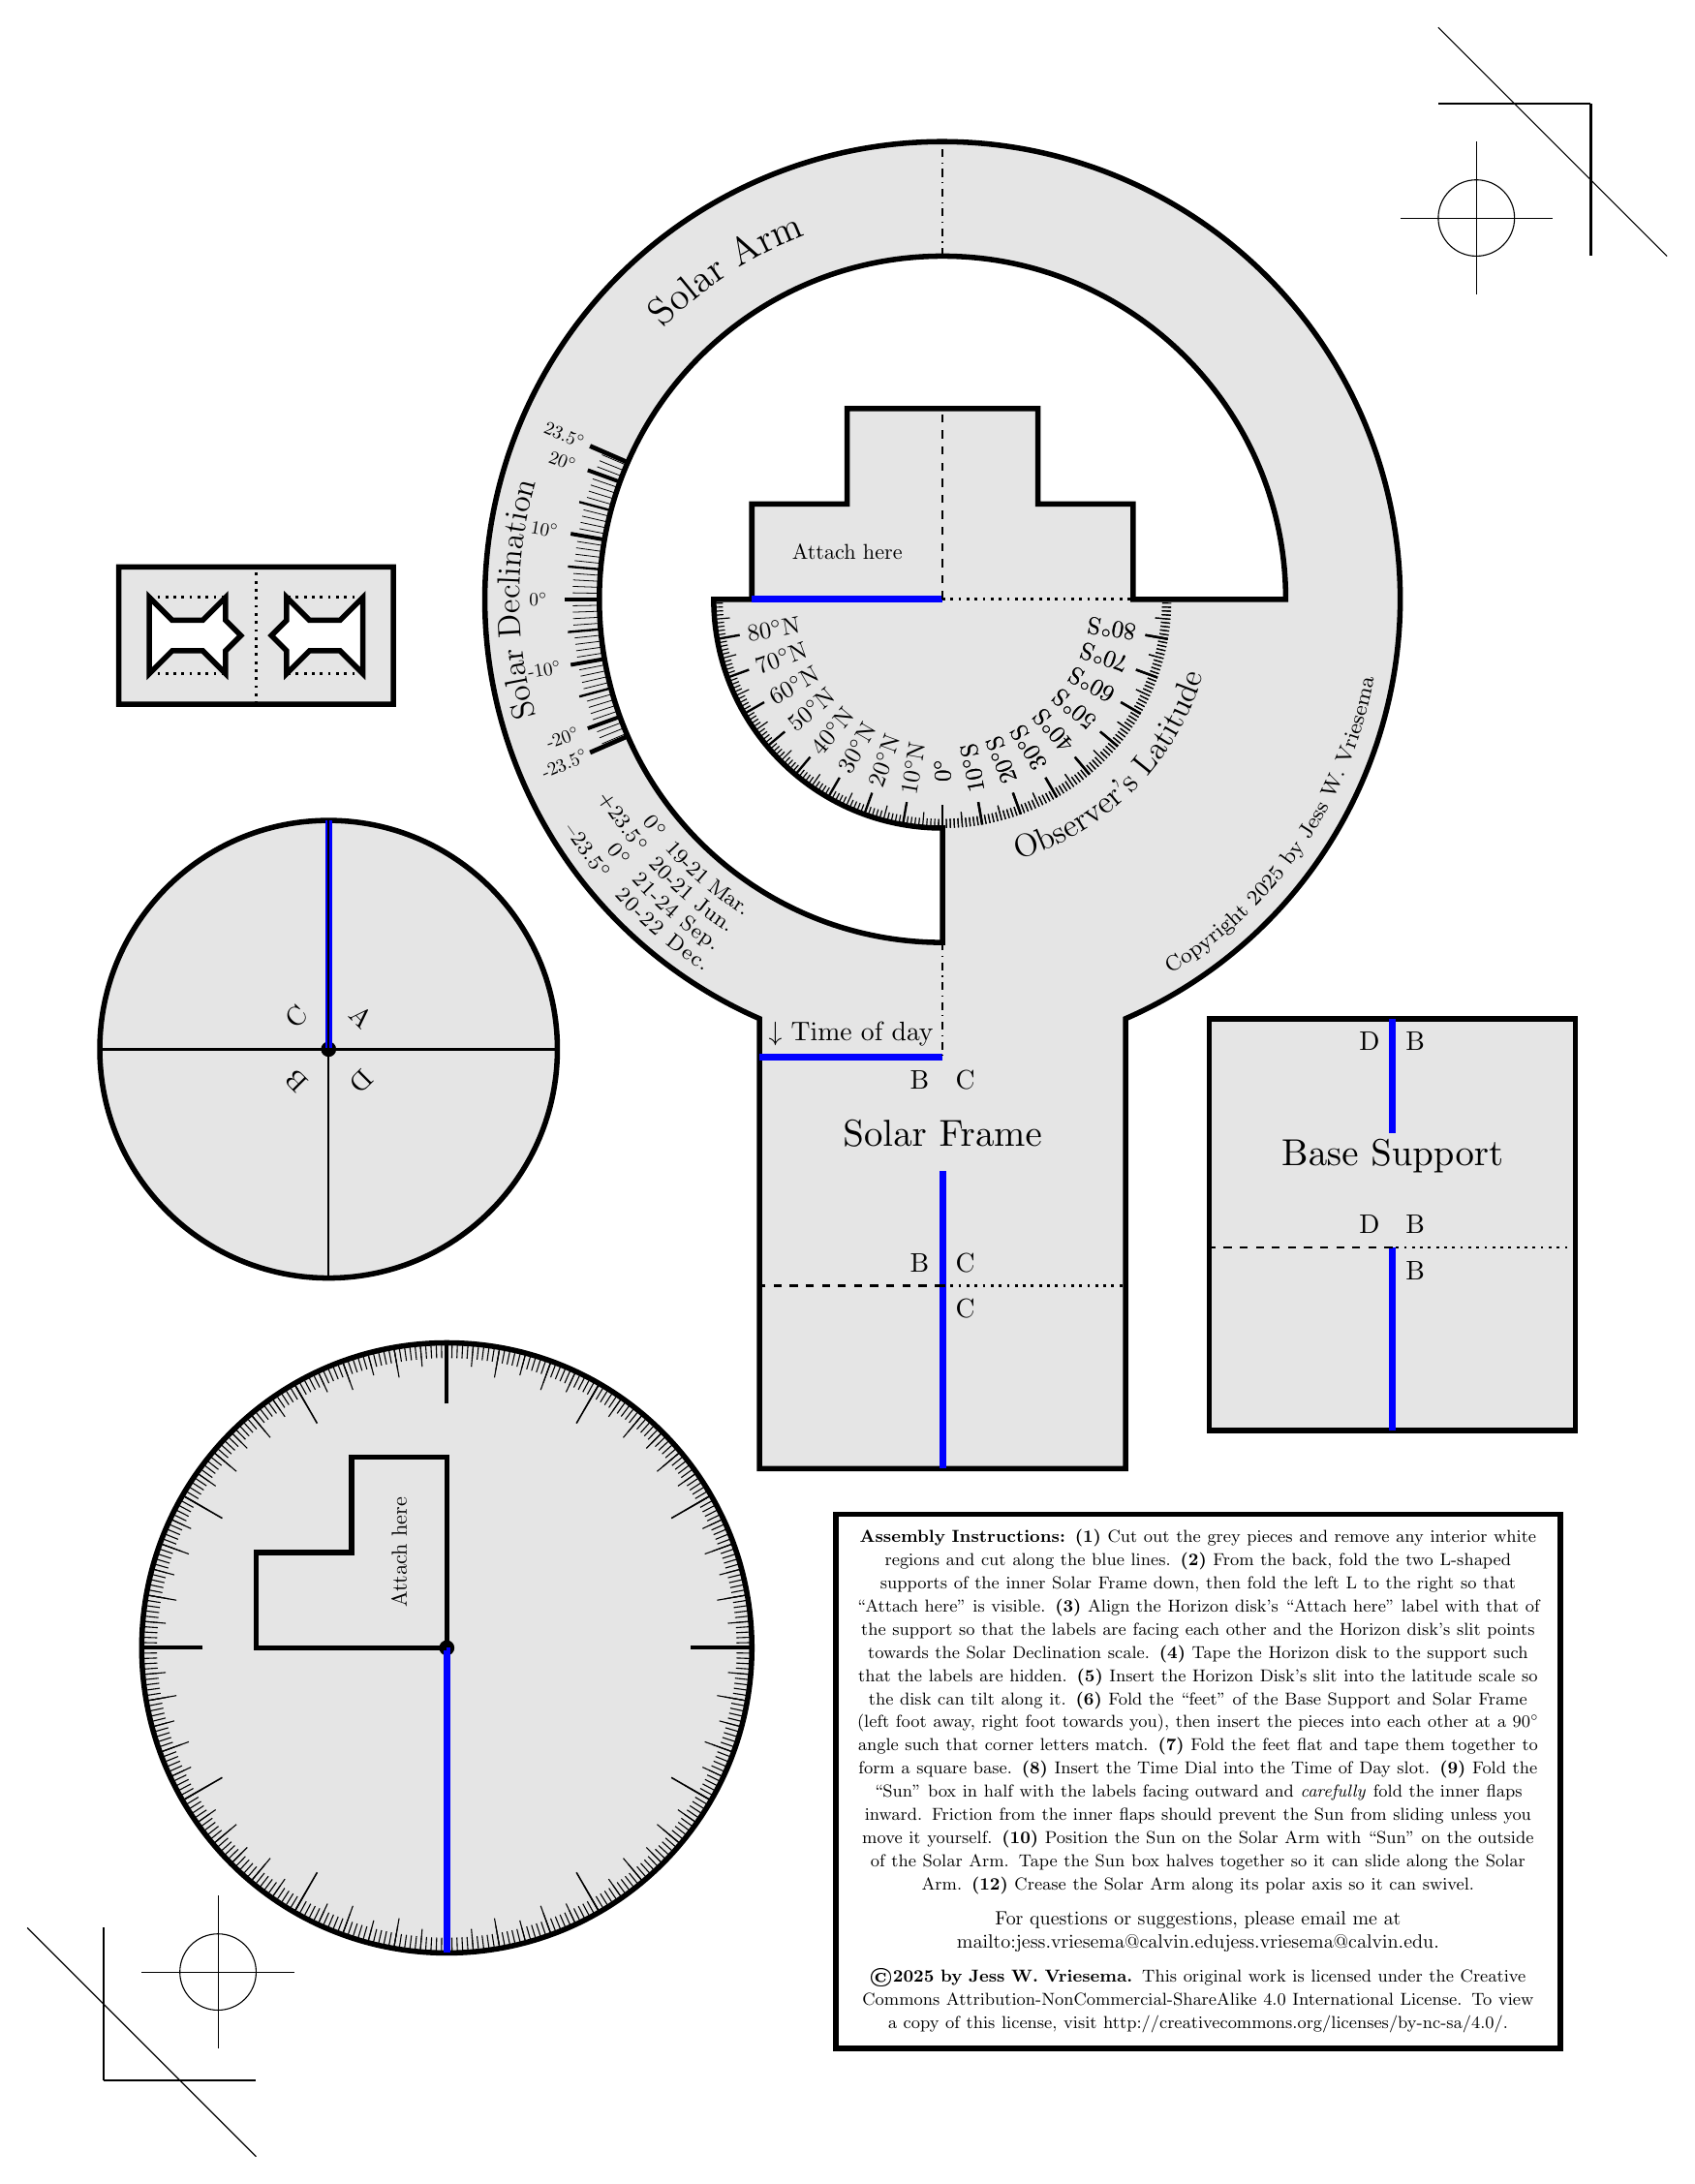
\begin{tikzpicture}%[overlay,remember picture]



%% ------------------------------------------------------------------------- %
%% Draw the QR CODE -- no flipping coordinates. 
%% ------------------------------------------------------------------------- %
%
%\begin{scope}[xshift=-\QRXShift,yshift=\QRYShift,rotate=\QRRotation]
%
%	\node at (0,0) {\includegraphics[width=2.5cm]{qr_to_website.png}};
%
%\end{scope}


\begin{scope}[xscale=-1]

\begin{scope}[xshift=\HelpCardXShift,yshift=\HelpCardYShift,rotate=\HelpCardRotation]
\node[font=\normalsize, text width=\HelpCardWidth/\HelpDiskTextScale-2*\HelpDiskTextMargin/\HelpDiskTextScale, scale=\HelpDiskTextScale] at (0,0) {
		\centering
		%Illustrated assembly instructions are available at \url{https://www.lpl.arizona.edu/~vriesema/solar_motion_instructions.php}. \\
		%\bigskip
		{\small \textbf{Assembly Instructions:} \textbf{(1)} Cut out the grey pieces and remove any interior white regions and cut along the blue lines. \textbf{(2)} From the back, fold the two L-shaped supports of the inner Solar Frame down, then fold the left L to the right so that ``Attach here'' is visible. \textbf{(3)} Align the Horizon disk's ``Attach here'' label with that of the support so that the labels are facing each other and the Horizon disk's slit points towards the Solar Declination scale. \textbf{(4)} Tape the Horizon disk to the support such that the labels are hidden. \textbf{(5)} Insert the Horizon Disk’s slit into the latitude scale so the disk can tilt along it. \textbf{(6)} Fold the ``feet'' of the Base Support and Solar Frame (left foot away, right foot towards you), then insert the pieces into each other at a 90{\degree} angle such that corner letters match. \textbf{(7)} Fold the feet flat and tape them together to form a square base. \textbf{(8)} Insert the Time Dial into the Time of Day slot. \textbf{(9)} Fold the ``Sun'' box in half with the labels facing outward and \emph{carefully} fold the inner flaps inward. Friction from the inner flaps should prevent the Sun from sliding unless you move it yourself. \textbf{(10)} Position the Sun on the Solar Arm with ``Sun'' on the outside of the Solar Arm. Tape the Sun box halves together so it can slide along the Solar Arm. \textbf{(12)} Crease the Solar Arm along its polar axis so it can swivel.} \\
		%\medskip
		%{\small Videos %, including an introduction, an assembly tutorial and examples, \\
		%will soon be available in the following YouTube playlist: \href{https://youtube.com/playlist?list=PL4fXsHwnHJ0unhdGVK-Qs-AM1HSjOCj5C}{https://youtube.com/playlist?list=PL4fXsHwnHJ0unhdGVK-Qs-AM1HSjOCj5C}.} \\
		%\bigskip
		%\textbf{Author's Note:} This papercraft model was inspired by the ``Solar Motion Demonstrator'' developed by J.L. Snider of Oberlin College in 1992, which I first encountered in a middle school science class. When I was preparing to teach Physics~115 at UW--Eau Claire, I could not find Snider's model, so I independently developed my own version of it.  It was designed to be cheap and easy to assemble.  I wish to thank Howard Turner of UW--Eau Claire for his help in developing this model.  This work is dedicated to curious students of astronomy, planetary science and Earth science, and those who teach them---especially those teachers with limited resources.  This model uses \emph{apparent solar time}, which ignores time zones and the equation of time. \\
		\medskip
		For questions or suggestions, please email me at \href{mailto:jess.vriesema@calvin.edu}{jess.vriesema@calvin.edu}. \\
		%Web page: \url{https://www.lpl.arizona.edu/~vriesema/} \\
		%Twitter: \url{https://twitter.com/Jvriesem} \\
		%TODO: \\
		\medskip
		%For more information, please visit \url{https://www.lpl.arizona.edu/~vriesema/solar_motion.php}. \\
		%\bigskip
		% \\
		%\medskip
		{\small \textbf{\copyright 2025 by Jess W. Vriesema.} This original work is licensed under the Creative Commons Attribution-NonCommercial-ShareAlike 4.0 International License. 
		To view a copy of this license, visit
 % fake URL that does not render as any text, but eats up a bug that causes the URL AFTER the Twitter URL to also point to Twitter. 
\url{http://creativecommons.org/licenses/by-nc-sa/4.0/}.} \\
	};
	\draw[line width=\HelpCardBorderWidth,color=\OutlineColor] (-\HelpCardWidth/2,-\HelpCardHeight/2) rectangle (\HelpCardWidth/2,\HelpCardHeight/2);
	
	\ifLaserCutterMode
		\draw[style=LaserCutterOutlineCut,line width=\LaserCutterLineWidth,color=\LaserCutterColor] (-\HelpCardWidth/2-\HelpCardBorderWidth/2+\LaserCutterLineWidth/2,-\HelpCardHeight/2-\HelpCardBorderWidth/2+\LaserCutterLineWidth/2) rectangle (\HelpCardWidth/2+\HelpCardBorderWidth/2-\LaserCutterLineWidth/2,\HelpCardHeight/2+\HelpCardBorderWidth/2-\LaserCutterLineWidth/2);
	\fi % \ifLaserCutterMode
	
\end{scope}


% ------------------------------------------------------------------------- %
% Draw the HORIZON DISK
% ------------------------------------------------------------------------- %
\begin{scope}[xshift=\HorizonDiskXShift,yshift=\HorizonDiskYShift,rotate=\HorizonDiskRotation]

% Draw the Horizon Disk
\draw[fill=\FillColor] circle[radius=\HorizonDiskRadius];
%\shade[shading=radial, inner color=white, outer color=gray!20] circle[radius=\HorizonDiskRadius];
\draw[color=\OutlineColor, line width=\OutlineWidth] (0,0) circle[radius=\HorizonDiskRadius];
\fill[color=black!100] (0,0) circle[radius=0.1cm];
% Unit ticks every 1 degree
\foreach \x in {0,1,...,359}
	\draw (\x:\HorizonDiskRadius-\HorizonDiskOneDegTickSize) -- (\x:\HorizonDiskRadius);
% Minor ticks every 30 degrees
\foreach \x in {0,5,...,355}
	\draw (\x:\HorizonDiskRadius-\HorizonDiskFiveDegTickSize) -- (\x:\HorizonDiskRadius);
% Intermediate ticks every 10 degrees
\foreach \x in {0,10,...,350}
	\draw (\x:\HorizonDiskRadius-\HorizonDiskTenDegTickSize) -- (\x:\HorizonDiskRadius);
% Major ticks with labels every 30 degrees
\foreach \x in {0,30,...,330}
	\draw[line width=\HorizonDiskThirtyDegTickWidth] (\x:\HorizonDiskRadius-\HorizonDiskThirtyDegTickSize) -- (\x:\HorizonDiskRadius);
%\foreach \x in {30,60,120,150,210,240,300,330}
%	\node[scale=\HorizonDiskThirtyDegLabelScale,font=\normalsize,rotate=\x] at (90-\x:\HorizonDiskRadius-\HorizonDiskThirtyDegTickSize-\HorizonDiskThirtyDegLabelOffset) {\x};
% Cardinal ticks with labels every 90 degrees
\foreach \x in {0,90,180,270}
	\draw[line width=\HorizonDiskNinetyDegTickWidth] (\x:\HorizonDiskRadius-\HorizonDiskNinetyDegTickSize) -- (\x:\HorizonDiskRadius);
%\node[scale=\HorizonDiskNinetyDegLabelScale,font=\normalsize] at (90:\HorizonDiskRadius-\HorizonDiskThirtyDegTickSize-2*\HorizonDiskNinetyDegLabelOffset) {N};
%\node[scale=\HorizonDiskNinetyDegLabelScale,font=\normalsize] at (0:\HorizonDiskRadius-\HorizonDiskThirtyDegTickSize-2*\HorizonDiskNinetyDegLabelOffset) {E};
%\node[scale=\HorizonDiskNinetyDegLabelScale,font=\normalsize] at (-90:\HorizonDiskRadius-\HorizonDiskThirtyDegTickSize-2*\HorizonDiskNinetyDegLabelOffset) {S};
%\node[scale=\HorizonDiskNinetyDegLabelScale,font=\normalsize] at (180:\HorizonDiskRadius-\HorizonDiskThirtyDegTickSize-2*\HorizonDiskNinetyDegLabelOffset) {W};
% Horizon Disk Label
%\node[scale=\HorizonDiskLabelScale] at (0,\HorizonDiskLabelRadius) {(backside)};
% Incision
\draw[color=\IncisionColor,line width=\HorizonDiskIncisionWidth] (0,0) -- (0,-\HorizonDiskRadius);

% Draw Solar Frame outline for attaching parts:
\draw[line width=\HorizonDiskSolarFrameLineWidth]
%	(-\HorizonDiskRadius,0)
	 (0,0) 
	-- (0,\SolarFrameCenterSupportFlapLength)
	-- (\SolarFrameCenterSupportFlapWidth,\SolarFrameCenterSupportFlapLength)
	-- (\SolarFrameCenterSupportFlapWidth,\SolarFrameCenterSupportFlapWidth)
	-- (\SolarFrameCenterSupportFlapLength,\SolarFrameCenterSupportFlapWidth)
	-- (\SolarFrameCenterSupportFlapLength,0)
	-- (\SolarFrameCenterSupportFlapWidth,0)
	-- (0,0);
%	-- (\SolarFrameCenterSupportFlapWidth,-\SolarFrameCenterSupportFlapLength)
%	-- (0,-\SolarFrameCenterSupportFlapLength)
%	-- (0,-\HorizonDiskRadius);
\node[scale=\HorizonDiskTapeMeScale,font=\normalsize,rotate=90] at (\SolarFrameCenterSupportFlapWidth/2,\SolarFrameCenterSupportFlapLength/2) {Attach here};

%\node[scale=\HorizonDiskTapeMeScale,font=\normalsize,rotate=0] at (-1.3*\SolarFrameCenterSupportFlapWidth,0) {\includegraphics[width=2.5cm]{qr_code_simple.png}};
%\node[scale=\HorizonDiskTapeMeScale,font=\normalsize,rotate=90] at (-\SolarFrameCenterSupportFlapWidth/3,0) {\bfseries{Scan for more info:}};

%}

% Laser cut mode
\ifLaserCutterMode
	\draw[style=LaserCutterOutlineCut,color=\LaserCutterColor,line width=\LaserCutterLineWidth] 
		({-90+asin(\HorizonDiskIncisionWidth/2/\HorizonDiskRadius-\LaserCutterLineWidth/2/\HorizonDiskRadius)}:\HorizonDiskRadius+\HorizonDiskIncisionWidth/2-\LaserCutterLineWidth/2)
		arc[start angle={-90+asin(\HorizonDiskIncisionWidth/2/\HorizonDiskRadius-\LaserCutterLineWidth/2/\HorizonDiskRadius)},end angle={270-asin(\HorizonDiskIncisionWidth/2/\HorizonDiskRadius-\LaserCutterLineWidth/2/\HorizonDiskRadius)},radius=\HorizonDiskRadius+\HorizonDiskIncisionWidth/2-\LaserCutterLineWidth/2]
		-- ({270-asin(\HorizonDiskIncisionWidth/2/\HorizonDiskRadius-\LaserCutterLineWidth/2/\HorizonDiskRadius)}:\HorizonDiskRadius+\HorizonDiskIncisionWidth/2-\LaserCutterLineWidth/2)
		-- (-\HorizonDiskIncisionWidth/2+\LaserCutterLineWidth/2,\HorizonDiskIncisionWidth/2-\LaserCutterLineWidth/2)
		-- (\HorizonDiskIncisionWidth/2-\LaserCutterLineWidth/2,\HorizonDiskIncisionWidth/2-\LaserCutterLineWidth/2)
		-- cycle;
\fi % \ifLaserCutterMode

% HELPER LINES
\ifPrintHelperLines
	\draw[
	  help lines,
	  line width=0.1pt,
	  blue
	] (-1.05*\HorizonDiskRadius, -1.05*\HorizonDiskRadius) grid[step={(1cm,1cm)}]  (1.05*\HorizonDiskRadius, 1.05*\HorizonDiskRadius);
\fi

\end{scope}




% ------------------------------------------------------------------------- %
% Draw the TIME DISK
% ------------------------------------------------------------------------- %
\begin{scope}[xshift=\TimeDiskXShift,yshift=\TimeDiskYShift,rotate=\TimeDiskRotation]

\draw[fill=\FillColor] circle[radius=\TimeDiskRadius];
%\shade[shading=radial, inner color=white, outer color=gray!20] circle[radius=\TimeDiskRadius];
\draw[color=\OutlineColor, line width=\OutlineWidth] (0,0) circle[radius=\TimeDiskRadius];
\fill[color=black!100] (0,0) circle[radius=0.1cm];
% Minor ticks every 1 hour
%\foreach \x in {0,15,...,345}
%	\draw (\x:\TimeDiskRadius-\TimeDiskHourTickSize) -- (\x:\TimeDiskRadius);
%\foreach \theta / \hour in {15/1, 30/2, 60/4, 75/5, 105/7, 120/8, 150/10, 165/11, 195/13, 210/14, 240/16, 255/17, 285/19, 300/20, 330/22, 345/23} {
%	\draw[line width=\TimeDiskHourTickWidth] (90-\theta:\TimeDiskRadius-\TimeDiskHourTickSize) -- (90-\theta:\TimeDiskRadius);
%	\node[scale=\TimeDiskHourLabelScale,font=\normalsize] at (90-\theta:\TimeDiskRadius-\TimeDiskHourTickSize-2*\TimeDiskHourLabelOffset) {\hour};
%}
%%\node[scale=\TimeDiskThreeHourLabelScale,font=\normalsize] at (90-15:\TimeDiskRadius-\TimeDiskThreeHourTickSize-2*\TimeDiskThreeHourLabelOffset) {1};
%% Intermediate ticks every 3 hours
%\foreach \x in {0,45,...,315}
%	\draw[line width=\TimeDiskThreeHourTickWidth] (\x:\TimeDiskRadius-\TimeDiskThreeHourTickSize) -- (\x:\TimeDiskRadius);
%\node[scale=\TimeDiskThreeHourLabelScale,font=\normalsize] at (90-45:\TimeDiskRadius-\TimeDiskThreeHourTickSize-2*\TimeDiskThreeHourLabelOffset) {3};
%\node[scale=\TimeDiskThreeHourLabelScale,font=\normalsize] at (90-135:\TimeDiskRadius-\TimeDiskThreeHourTickSize-2*\TimeDiskThreeHourLabelOffset) {9};
%\node[scale=\TimeDiskThreeHourLabelScale,font=\normalsize] at (90-225:\TimeDiskRadius-\TimeDiskThreeHourTickSize-2*\TimeDiskThreeHourLabelOffset) {15};
%\node[scale=\TimeDiskThreeHourLabelScale,font=\normalsize] at (90-315:\TimeDiskRadius-\TimeDiskThreeHourTickSize-2*\TimeDiskThreeHourLabelOffset) {21};
%
%% Cardinal ticks with labels every 90 degrees
%\foreach \x in {90,180,270}
%	\draw[line width=\TimeDiskCardinalHourTickWidth] (90-\x:\TimeDiskRadius-\TimeDiskCardinalHourTickSize) -- (90-\x:\TimeDiskRadius);
%%\node[scale=\TimeDiskCardinalHourLabelScale,font=\normalsize] at (90:\TimeDiskRadius-\TimeDiskCardinalHourTickSize-2*\TimeDiskCardinalHourLabelOffset) {24};
%\node[scale=\TimeDiskCardinalHourLabelScale,font=\normalsize] at (0:\TimeDiskRadius-\TimeDiskCardinalHourTickSize-2*\TimeDiskCardinalHourLabelOffset) {6};
%\node[scale=\TimeDiskCardinalHourLabelScale,font=\normalsize] at (-90:\TimeDiskRadius-\TimeDiskCardinalHourTickSize-2*\TimeDiskCardinalHourLabelOffset) {12};
%\node[scale=\TimeDiskCardinalHourLabelScale,font=\normalsize] at (180:\TimeDiskRadius-\TimeDiskCardinalHourTickSize-2*\TimeDiskCardinalHourLabelOffset) {18};

% Incision
\draw[color=\IncisionColor,line width=\TimeDiskIncisionWidth] (90-180:\TimeDiskIncisionExtraSize) -- (90-0:\TimeDiskRadius);

% Helper lines (to assist with footer construction alignment when taping)
\draw[line width=\TimeDiskUndersideAlignmentLineWidth] 
	(-\TimeDiskRadius,0) --  (\TimeDiskRadius,0);  % horizontal (3/9, E/W) alignment line
\draw[line width=\TimeDiskUndersideAlignmentLineWidth] 
	(0,-\TimeDiskRadius) --  (0,\TimeDiskRadius);  % vertical (6/12, N/S) alignment line
	
% "Time"
%\node[scale=\TimeDiskLabelScale,font=\normalsize] at (0,-\TimeDiskLabelRadius) {Time Dial};
%\draw[decoration={text along path,
%      text={|\normalsize|T i m e},text align={center},text color=black,raise=0.0cm},decorate] (90-270:\TimeDiskLabelRadius) arc[start angle=90-270,end angle=90-90,radius=\TimeDiskLabelRadius];

% Footer clues
\node[scale=\SolarFrameFootLabelScale,font=\normalsize,rotate=-45] at (135:2*\FooterSupportLabelOffset) {A};
\node[scale=\SolarFrameFootLabelScale,font=\normalsize,rotate=-135] at (225:2*\FooterSupportLabelOffset) {D};
\node[scale=\SolarFrameFootLabelScale,font=\normalsize,rotate=45] at (45:2*\FooterSupportLabelOffset) {C};
\node[scale=\SolarFrameFootLabelScale,font=\normalsize,rotate=135] at (315:2*\FooterSupportLabelOffset) {B};

% Laser cut mode
\ifLaserCutterMode
	\draw[style=LaserCutterOutlineCut,color=\LaserCutterColor,line width=\LaserCutterLineWidth] 
		(-\TimeDiskIncisionWidth/2+\LaserCutterLineWidth/2,-\TimeDiskIncisionWidth/2+\LaserCutterLineWidth/2)
		-- ({-270+asin(\TimeDiskIncisionWidth/2/\TimeDiskRadius-\LaserCutterLineWidth/2/\TimeDiskRadius)}:\TimeDiskRadius+\OutlineWidth/2-\LaserCutterLineWidth/2) 
		 arc[start angle={-270+asin(\TimeDiskIncisionWidth/2/\TimeDiskRadius-\LaserCutterLineWidth/2/\TimeDiskRadius)}, end angle={90-asin(\TimeDiskIncisionWidth/2/\TimeDiskRadius-\LaserCutterLineWidth/2/\TimeDiskRadius)}, radius=\TimeDiskRadius+\OutlineWidth/2-\LaserCutterLineWidth/2]
		-- (\TimeDiskIncisionWidth/2-\LaserCutterLineWidth/2,-\TimeDiskIncisionWidth/2+\LaserCutterLineWidth/2)
		-- cycle;
\fi % \ifLaserCutterMode

% HELPER LINES
\ifPrintHelperLines
	\draw[
	  help lines,
	  line width=0.1pt,
	  blue
	] (-1.05*\TimeDiskRadius, -1.05*\TimeDiskRadius) grid[step={(1cm,1cm)}]  (1.05*\TimeDiskRadius, 1.05*\TimeDiskRadius);
\fi

\end{scope}




% ------------------------------------------------------------------------- %
% Draw the Sun Carriage
% ------------------------------------------------------------------------- %
\begin{scope}[xshift=\SunCarriageXShift,yshift=\SunCarriageYShift,rotate=\SunCarriageRotation]

%% Draw the Sun Carriage (in this thing to save space)
%\draw[color=\OutlineColor,fill=\FillColor,even odd rule,line width=\OutlineWidth] 
%	(-\SunCarriageWidth,0) rectangle (\SunCarriageWidth,\SunCarriageHeight)
%	(-\SunCarriageWidth+\SunCarriageInternalWidth,\SunCarriageInternalWidth) rectangle (-\SunCarriageInternalWidth,\SunCarriageWidth-\SunCarriageInternalWidth)
%	(\SunCarriageInternalWidth,\SunCarriageInternalWidth) rectangle (\SunCarriageWidth-\SunCarriageInternalWidth,\SunCarriageWidth-\SunCarriageInternalWidth);

	
	
	% Try drawing Sun Carriage without rects specifically
	\draw[color=\OutlineColor,fill=\FillColor,even odd rule,line width=\OutlineWidth] 
		(-\SunCarriageWidth,0) rectangle (\SunCarriageWidth,\SunCarriageHeight) % Outer outline
		% Left hole
		(-\SunCarriageWidth+\SunCarriageInternalWidth,\SunCarriageInternalWidth) % bottom left corner
			-- (-\SunCarriageWidth+\SunCarriageInternalWidth,\SunCarriageHeight-\SunCarriageInternalWidth) % top left corner
			-- (-\SunCarriageWidth+\SunCarriageInternalWidth+\SunCarriageFlapWidth,\SunCarriageHeight-\SunCarriageInternalWidth-\SunCarriageFlapWidth) % top flap left vertex
			-- (-\SunCarriageInternalWidth-\SunCarriageFlapWidth,\SunCarriageHeight-\SunCarriageInternalWidth-\SunCarriageFlapWidth) % top flap right vertex
			-- (-\SunCarriageInternalWidth,\SunCarriageHeight-\SunCarriageInternalWidth) % top right corner
			-- (-\SunCarriageInternalWidth,\SunCarriageHeight/2+\SunCarriageIndicatorSize) % right-top
			-- (-\SunCarriageInternalWidth+\SunCarriageIndicatorSize,\SunCarriageHeight/2) % right-point
			-- (-\SunCarriageInternalWidth,\SunCarriageHeight/2-\SunCarriageIndicatorSize) % right-bot
			-- (-\SunCarriageInternalWidth,\SunCarriageInternalWidth) % bottom right corner
			-- (-\SunCarriageInternalWidth-\SunCarriageFlapWidth,\SunCarriageInternalWidth+\SunCarriageFlapWidth) % bottom flap right vertex
			-- (-\SunCarriageWidth+\SunCarriageInternalWidth+\SunCarriageFlapWidth,\SunCarriageInternalWidth+\SunCarriageFlapWidth) % bottom flap left vertex
			-- (-\SunCarriageWidth+\SunCarriageInternalWidth,\SunCarriageInternalWidth) % bottom
			-- cycle
		% Right hole
		(\SunCarriageWidth-\SunCarriageInternalWidth,\SunCarriageInternalWidth) % bottom right corner
			-- (\SunCarriageWidth-\SunCarriageInternalWidth,\SunCarriageHeight-\SunCarriageInternalWidth) % top right corner
			-- (\SunCarriageWidth-\SunCarriageInternalWidth-\SunCarriageFlapWidth,\SunCarriageHeight-\SunCarriageInternalWidth-\SunCarriageFlapWidth) % top flap right vertex
			-- (\SunCarriageInternalWidth+\SunCarriageFlapWidth,\SunCarriageHeight-\SunCarriageInternalWidth-\SunCarriageFlapWidth) % top flap left vertex
			-- (\SunCarriageInternalWidth,\SunCarriageHeight-\SunCarriageInternalWidth) % top left corner
			-- (\SunCarriageInternalWidth,\SunCarriageHeight/2+\SunCarriageIndicatorSize) % left-top
			-- (\SunCarriageInternalWidth-\SunCarriageIndicatorSize,\SunCarriageHeight/2) % left-point
			-- (\SunCarriageInternalWidth,\SunCarriageHeight/2-\SunCarriageIndicatorSize) % left-bot
			-- (\SunCarriageInternalWidth,\SunCarriageInternalWidth) % bottom left corner
			-- (\SunCarriageInternalWidth+\SunCarriageFlapWidth,\SunCarriageInternalWidth+\SunCarriageFlapWidth) % bottom flap left vertex
			-- (\SunCarriageWidth-\SunCarriageInternalWidth-\SunCarriageFlapWidth,\SunCarriageInternalWidth+\SunCarriageFlapWidth) % bottom flap right vertex
			-- (\SunCarriageWidth-\SunCarriageInternalWidth,\SunCarriageInternalWidth) % bottom
			-- cycle; 
			
			
	% Fold lines
	\draw[\valleyFold,line width=1pt]
		(0,0) -- (0,\SunCarriageHeight); % Folds Solar Carriage in half
	\draw[\valleyFold,line width=1pt]
		(-\SunCarriageWidth+\SunCarriageInternalWidth,\SunCarriageHeight-\SunCarriageInternalWidth) -- (-\SunCarriageInternalWidth,\SunCarriageHeight-\SunCarriageInternalWidth); % left cell top flap 
	\draw[\valleyFold,line width=1pt]
		(\SunCarriageWidth-\SunCarriageInternalWidth,\SunCarriageHeight-\SunCarriageInternalWidth) -- (\SunCarriageInternalWidth,\SunCarriageHeight-\SunCarriageInternalWidth); % right cell top flap 
	\draw[\valleyFold,line width=1pt]
		(-\SunCarriageWidth+\SunCarriageInternalWidth,\SunCarriageInternalWidth) -- (-\SunCarriageInternalWidth,\SunCarriageInternalWidth); % left cell bottom flap 
	\draw[\valleyFold,line width=1pt]
		(\SunCarriageWidth-\SunCarriageInternalWidth,\SunCarriageInternalWidth) -- (\SunCarriageInternalWidth,\SunCarriageInternalWidth); % right cell bottom flap 
	
	
%% Indicator lines
%\draw[line width=1pt]
%	(-\SunCarriageInternalWidth,\SunCarriageHeight/2) -- (\SunCarriageInternalWidth,\SunCarriageHeight/2);
%\draw[line width=1pt]
%	(-\SunCarriageWidth,\SunCarriageHeight/2) -- (-\SunCarriageWidth+\SunCarriageInternalWidth,\SunCarriageHeight/2);
%\draw[line width=1pt]
%	(\SunCarriageWidth,\SunCarriageHeight/2) -- (\SunCarriageWidth-\SunCarriageInternalWidth,\SunCarriageHeight/2);

%% Draw hole punch locations (left side)
%\drawHolePunch{-\SunCarriageInternalWidth-\SunCarriageInternalCircleRadii}{\SunCarriageInternalWidth+\SunCarriageInternalCircleRadii};
%\drawHolePunch{-\SunCarriageWidth+\SunCarriageInternalWidth+\SunCarriageInternalCircleRadii}{\SunCarriageInternalWidth+\SunCarriageInternalCircleRadii};
%\drawHolePunch{-\SunCarriageInternalWidth-\SunCarriageInternalCircleRadii}{\SunCarriageHeight-\SunCarriageInternalWidth-\SunCarriageInternalCircleRadii};
%\drawHolePunch{-\SunCarriageWidth+\SunCarriageInternalWidth+\SunCarriageInternalCircleRadii}{\SunCarriageHeight-\SunCarriageInternalWidth-\SunCarriageInternalCircleRadii};
%% Draw hole punch locations (right side)
%\drawHolePunch{\SunCarriageInternalWidth+\SunCarriageInternalCircleRadii}{\SunCarriageInternalWidth+\SunCarriageInternalCircleRadii};
%\drawHolePunch{\SunCarriageWidth-\SunCarriageInternalWidth-\SunCarriageInternalCircleRadii}{\SunCarriageInternalWidth+\SunCarriageInternalCircleRadii};
%\drawHolePunch{\SunCarriageInternalWidth+\SunCarriageInternalCircleRadii}{\SunCarriageHeight-\SunCarriageInternalWidth-\SunCarriageInternalCircleRadii};
%\drawHolePunch{\SunCarriageWidth-\SunCarriageInternalWidth-\SunCarriageInternalCircleRadii}{\SunCarriageHeight-\SunCarriageInternalWidth-\SunCarriageInternalCircleRadii};


% Laser cut mode
\ifLaserCutterMode
	\draw[style=LaserCutterOutlineCut,color=\LaserCutterColor, line width=\LaserCutterLineWidth] 
	(-\SunCarriageWidth-\OutlineWidth/2+\LaserCutterLineWidth/2,-\OutlineWidth/2+\LaserCutterLineWidth/2) rectangle (\SunCarriageWidth+\OutlineWidth/2-\LaserCutterLineWidth/2,\SunCarriageHeight+\OutlineWidth/2-\LaserCutterLineWidth/2);

	\draw[style=LaserCutterCut,color=\LaserCutterColor, line width=\LaserCutterLineWidth] 	
	(-\SunCarriageWidth+\SunCarriageInternalWidth+\OutlineWidth/2-\LaserCutterLineWidth/2,\SunCarriageInternalWidth+\OutlineWidth/2-\LaserCutterLineWidth/2) rectangle (-\SunCarriageInternalWidth-\OutlineWidth/2+\LaserCutterLineWidth/2,\SunCarriageWidth-\SunCarriageInternalWidth-\OutlineWidth/2+\LaserCutterLineWidth/2);
	
	\draw[style=LaserCutterCut,color=\LaserCutterColor, line width=\LaserCutterLineWidth] 	
	(\SunCarriageWidth-\SunCarriageInternalWidth-\OutlineWidth/2+\LaserCutterLineWidth/2,\SunCarriageInternalWidth+\OutlineWidth/2-\LaserCutterLineWidth/2) rectangle (\SunCarriageInternalWidth+\OutlineWidth/2-\LaserCutterLineWidth/2,\SunCarriageWidth-\SunCarriageInternalWidth-\OutlineWidth/2+\LaserCutterLineWidth/2);
	
\draw[style=LaserCutterFoldAid,color=\LaserCutterColor,line width=\LaserCutterLineWidth]
	(0,0) -- (0,\SunCarriageHeight);
	
\fi % \ifLaserCutterM\SolarFrameFootLengthode

% HELPER LINES
\ifPrintHelperLines
	\draw[
	  help lines,
	  line width=0.1pt,
	  blue
	] (-1.05*\SolarFrameFootLength, -0.05*\SolarFrameFootHeight) grid[step={(1cm,1cm)}]  (1.05*\SolarFrameFootLength, 1.05*\SolarFrameFootHeight);
\fi

\end{scope}





% ------------------------------------------------------------------------- %
% Draw the SOLAR FRAME
% ------------------------------------------------------------------------- %
\begin{scope}[xshift=\SolarFrameXShift,yshift=\SolarFrameYShift,rotate=\SolarFrameRotation]
% Draw the Solar Frame
\draw[color=\OutlineColor,fill=\FillColor,even odd rule,line width=\OutlineWidth] 
	(0,-\SolarFrameOuterRadius-\SolarFrameFootHeight-\SolarFrameExtraFootHeight)
	-|
	({270-asin(\SolarFrameFootLength/\SolarFrameOuterRadius)}:\SolarFrameOuterRadius) arc[start angle={270-asin(\SolarFrameFootLength/\SolarFrameOuterRadius)},end angle={-90+asin(\SolarFrameFootLength/\SolarFrameOuterRadius)},radius=\SolarFrameOuterRadius]
	|- cycle                                  
	(-\SolarFrameInnerRadius,0) arc[start angle=180,end angle=-90,radius=\SolarFrameInnerRadius] 
	-- (0,-\SolarFrameCenterLatitudeArcRadius)
	arc[start angle=-90,end angle=0,radius=\SolarFrameCenterLatitudeArcRadius] %(\SolarFrameCenterLatitudeArcRadius,0)
	-- (\SolarFrameCenterSupportFlapLength,0)
	-- (\SolarFrameCenterSupportFlapLength,\SolarFrameCenterSupportFlapWidth)
	-- (\SolarFrameCenterSupportFlapWidth,\SolarFrameCenterSupportFlapWidth)
	-- (\SolarFrameCenterSupportFlapWidth,\SolarFrameCenterSupportFlapLength)
	-- (-\SolarFrameCenterSupportFlapWidth,\SolarFrameCenterSupportFlapLength)
	-- (-\SolarFrameCenterSupportFlapWidth,\SolarFrameCenterSupportFlapWidth)
	-- (-\SolarFrameCenterSupportFlapLength,\SolarFrameCenterSupportFlapWidth) 
	-- (-\SolarFrameCenterSupportFlapLength,0) 
	-- cycle; %(-\SolarFrameInnerRadius,0)


% Incision for the Time Disk
\draw[color=\IncisionColor,line width=\SolarFrameTimeDiskIncisionWidth]
	(0,-\SolarFrameOuterRadius) -- (\SolarFrameFootLength,-\SolarFrameOuterRadius);
% Incision for the Foot Support
\draw[color=\IncisionColor,line width=\SolarFrameTimeDiskIncisionWidth]
	(0,-\SolarFrameOuterRadius-\SolarFrameFootHeight/2) -- (0,-\SolarFrameOuterRadius-\SolarFrameFootHeight-\SolarFrameExtraFootHeight);
% Incision for horizon support flap
\draw[color=\IncisionColor,line width=\SolarFrameTimeDiskIncisionWidth] (0,0) -- (\SolarFrameCenterSupportFlapLength,0);
% Attach here label
\node[scale=\HorizonDiskTapeMeScale,font=\normalsize] at (\SolarFrameCenterSupportFlapLength/2,\SolarFrameCenterSupportFlapWidth/2) {Attach here};

%% Markings for Solar Declination
%% Major declination markers
%\foreach \x in {-\axialTilt,0,+\axialTilt}
%{
%	\draw[line width=\SolarFrameDeclinationMajorLineWidth] (\x:\SolarFrameInnerRadius) --  (\x:\SolarFrameDeclinationMajorLineLength+\SolarFrameInnerRadius);
%	\node[scale=\SolarFrameDeclinationMajorLineLabelScale,font=\normalsize,rotate=-\x] at (\x:\SolarFrameDeclinationMajorLineLength+\SolarFrameInnerRadius+\SolarFrameDeclinationMajorLineLabelOffset) {\x{\degree}};
%}
%% Minor declination markers
%\foreach \x in {-20,-10,10,20} 
%{
%	\draw[line width=\SolarFrameDeclinationMinorLineWidth] (\x:\SolarFrameInnerRadius) --  (\x:\SolarFrameDeclinationMinorLineLength+\SolarFrameInnerRadius);
%	\node[scale=\SolarFrameDeclinationMinorLineLabelScale,font=\normalsize,rotate=-\x] at (\x:\SolarFrameDeclinationMinorLineLength+\SolarFrameInnerRadius+\SolarFrameDeclinationMinorLineLabelOffset) {\x{\degree}};
%}

	%%%%%%%%%%%%%%%%%
% Markings for Solar Declination
	% Minor declination markers (unlabelled)
	\pgfmathsetmacro{\floorAxialTilt}{int(floor(\axialTilt))}
	\foreach \x in {-\floorAxialTilt,...,+\floorAxialTilt} 
	{
		% Is it a major declination marker?
		\pgfmathparse{mod(\x,10)}
		\ifnum0=\pgfmathresult\relax
			% major -- big, thick and labelled
			\draw[line width=\SolarFrameDeclinationMajorLineWidth] (\x:\SolarFrameInnerRadius) --  (\x:\SolarFrameDeclinationMajorLineLength+\SolarFrameInnerRadius);
			\node[scale=\SolarFrameDeclinationMajorLineLabelScale,font=\normalsize,rotate=-\x] at (\x:\SolarFrameDeclinationMajorLineLength+\SolarFrameInnerRadius+\SolarFrameDeclinationMajorLineLabelOffset) {\x{\degree}};
		\else
			\pgfmathparse{mod(\x,5)}
			\ifnum0=\pgfmathresult\relax
				% Medium: thicker, bigger lines, but no label
				\draw[line width=\SolarFrameDeclinationMedLineWidth] (\x:\SolarFrameInnerRadius) --  (\x:\SolarFrameDeclinationMedLineLength+\SolarFrameInnerRadius);
				%\node[scale=\SolarFrameDeclinationMedLineLabelScale,font=\normalsize,rotate=\x] at (\x:\SolarFrameDeclinationMedLineLength+\SolarFrameInnerRadius+\SolarFrameDeclinationMedLineLabelOffset) {};
			\else
				% minor -- thin, short lines, no label
				\draw[line width=\SolarFrameDeclinationMinorLineWidth] (\x:\SolarFrameInnerRadius) --  (\x:\SolarFrameDeclinationMinorLineLength+\SolarFrameInnerRadius);
			\fi
		\fi
	}
	% Axial Tilt markers (labelled)
	\foreach \x in {-\axialTilt,\axialTilt}
	{
		\draw[line width=1.2*\SolarFrameDeclinationMajorLineWidth] (\x:\SolarFrameInnerRadius) --  (\x:1.2*\SolarFrameDeclinationMajorLineLength+\SolarFrameInnerRadius);
		\node[scale=\SolarFrameDeclinationMajorLineLabelScale,font=\normalsize,rotate=-\x] at (\x:\SolarFrameDeclinationMajorLineLength+\SolarFrameInnerRadius+1.3*\SolarFrameDeclinationMajorLineLabelOffset) {\x{\degree}};
	}
	%%%%%%%%%%%%%%%%%


% Solar declination label
\draw[decoration={text along path,
      text={|\large|Solar Declination},text align={center},text color=black,raise=0.0cm},decorate] (-90:\SolarFrameDeclinationLabelRadius) arc[start angle=-90,end angle=90,radius=\SolarFrameDeclinationLabelRadius];
      
\draw[decoration={text along path,
      text={|\Large|Solar Arm},text align={center},text color=black,raise=0.0cm},decorate] (\axialTilt:0.4*\SolarFrameOuterRadius+0.6*\SolarFrameInnerRadius) arc[start angle=\axialTilt,end angle=90,radius=0.4*\SolarFrameOuterRadius+0.6*\SolarFrameInnerRadius];
      
%      \draw[decoration={text along path,
%	      text={|\large|Solar Arm},text align={center},text color=black,raise=0.0cm},decorate] (90:0.4*\SolarFrameOuterRadius+0.6*\SolarFrameInnerRadius) arc[start angle=90,end angle=\axialTilt,radius=0.4*\SolarFrameOuterRadius+0.6*\SolarFrameInnerRadius];
	      
	
	\draw[decoration={text along path,
	      text={|\footnotesize|{0{\degree}}},text align={right},text color=black,raise=0.2cm},decorate] (-35:0.4*\SolarFrameOuterRadius+0.6*\SolarFrameInnerRadius) arc[start angle=-35,end angle=-40,radius=0.4*\SolarFrameOuterRadius+0.6*\SolarFrameInnerRadius];
	\draw[decoration={text along path,
	      text={|\footnotesize|{+23.5{\degree}}},text align={right},text color=black,raise=-0.1cm},decorate] (-35:0.4*\SolarFrameOuterRadius+0.6*\SolarFrameInnerRadius) arc[start angle=-35,end angle=-40,radius=0.4*\SolarFrameOuterRadius+0.6*\SolarFrameInnerRadius];
	\draw[decoration={text along path,
	      text={|\footnotesize|{0{\degree}}},text align={right},text color=black,raise=-0.4cm},decorate] (-35:0.4*\SolarFrameOuterRadius+0.6*\SolarFrameInnerRadius) arc[start angle=-35,end angle=-40,radius=0.4*\SolarFrameOuterRadius+0.6*\SolarFrameInnerRadius];
	\draw[decoration={text along path,
	      text={|\footnotesize|{--23.5{\degree}}},text align={right},text color=black,raise=-0.7cm},decorate] (-35:0.4*\SolarFrameOuterRadius+0.6*\SolarFrameInnerRadius) arc[start angle=-35,end angle=-40,radius=0.4*\SolarFrameOuterRadius+0.6*\SolarFrameInnerRadius];
	      
	\draw[decoration={text along path,
	      text={|\footnotesize|19-21 Mar.},text align={left},text color=black,raise=0.2cm},decorate] (-42:0.4*\SolarFrameOuterRadius+0.6*\SolarFrameInnerRadius) arc[start angle=-42,end angle=-60,radius=0.4*\SolarFrameOuterRadius+0.6*\SolarFrameInnerRadius];
	\draw[decoration={text along path,
	      text={|\footnotesize|20-21 Jun.},text align={left},text color=black,raise=-0.1cm},decorate] (-42:0.4*\SolarFrameOuterRadius+0.6*\SolarFrameInnerRadius) arc[start angle=-42,end angle=-60,radius=0.4*\SolarFrameOuterRadius+0.6*\SolarFrameInnerRadius];
	\draw[decoration={text along path,
	      text={|\footnotesize|21-24 Sep.},text align={left},text color=black,raise=-0.4cm},decorate] (-42:0.4*\SolarFrameOuterRadius+0.6*\SolarFrameInnerRadius) arc[start angle=-42,end angle=-60,radius=0.4*\SolarFrameOuterRadius+0.6*\SolarFrameInnerRadius];
	\draw[decoration={text along path,
	      text={|\footnotesize|20-22 Dec.},text align={left},text color=black,raise=-0.7cm},decorate] (-42:0.4*\SolarFrameOuterRadius+0.6*\SolarFrameInnerRadius) arc[start angle=-42,end angle=-60,radius=0.4*\SolarFrameOuterRadius+0.6*\SolarFrameInnerRadius];
      
%\draw[decoration={text along path,
%      text={|\large|Rotate to show daily path of Sun},text align={center},text color=black,raise=0.0cm},decorate] (90:\SolarFrameDeclinationLabelRadius) arc[start angle=0,end angle=-90,radius=\SolarFrameDeclinationLabelRadius];

% Draw dashed lines for folding
\draw[\mountainAndValleyFold,line width=1pt] (0,\SolarFrameInnerRadius) -- (0,\SolarFrameOuterRadius);
\draw[\mountainAndValleyFold,line width=1pt] (0,-\SolarFrameInnerRadius) -- (0,-\SolarFrameOuterRadius);
\draw[\valleyFold,line width=1pt] (0,0) -- (-\SolarFrameCenterSupportFlapLength,0);
\draw[\mountainFold,line width=1pt] (0,0) -- (0,\SolarFrameCenterSupportFlapLength);
\draw[\mountainFold,line width=1pt] (0,-\SolarFrameOuterRadius-\SolarFrameFootHeight) -- (\SolarFrameFootLength,-\SolarFrameOuterRadius-\SolarFrameFootHeight);
\draw[\valleyFold,line width=1pt] (0,-\SolarFrameOuterRadius-\SolarFrameFootHeight) -- (-\SolarFrameFootLength,-\SolarFrameOuterRadius-\SolarFrameFootHeight);
%\SolarFrameExtraFootHeight

%% Latitude Lines
%\foreach \x in {10,20,...,80} 
%{
%	% Northern latitudes
%	\draw[line width=\SolarFrameLatitudeMajorLineWidth] (-90+\x:\SolarFrameCenterLatitudeArcRadius) --  (-90+\x:\SolarFrameCenterLatitudeArcRadius-\SolarFrameLatitudeMajorLineLength);
%	\node[scale=\SolarFrameLatitudeMajorLineLabelScale,font=\normalsize,rotate=90-\x] at (-90+\x:\SolarFrameCenterLatitudeArcRadius-\SolarFrameLatitudeMajorLineLength-\SolarFrameLatitudeMajorLineLabelOffset) {\x{\degree}N};
%	% Southern latitudes
%	\draw[line width=\SolarFrameLatitudeMajorLineWidth] (-90-\x:\SolarFrameCenterLatitudeArcRadius) --  (-90-\x:\SolarFrameCenterLatitudeArcRadius-\SolarFrameLatitudeMajorLineLength);
%	\node[scale=\SolarFrameLatitudeMajorLineLabelScale,font=\normalsize,rotate=90+\x] at (270-\x:\SolarFrameCenterLatitudeArcRadius-\SolarFrameLatitudeMajorLineLength-\SolarFrameLatitudeMajorLineLabelOffset) {\x{\degree}S};
%}
%% Equator
%\draw[line width=\SolarFrameLatitudeMajorLineWidth] (-90:\SolarFrameCenterLatitudeArcRadius) --  (-90:\SolarFrameCenterLatitudeArcRadius-\SolarFrameLatitudeMajorLineLength);
%\node[scale=\SolarFrameLatitudeMajorLineLabelScale,font=\normalsize,rotate=-90] at (-90:\SolarFrameCenterLatitudeArcRadius-\SolarFrameLatitudeMajorLineLength-\SolarFrameLatitudeMajorLineLabelOffset) {$0^\circ$}; %{Equator};


	% Minor latitude markers (unlabelled)
	\foreach \x in {-89,...,1,...,+89} 
	{
		% Is it a major declination marker?
		\pgfmathparse{mod(\x,10)}
		\ifnum0=\pgfmathresult\relax
			% major -- big, thick and labelled
			\draw[line width=\SolarFrameLatitudeMajorLineWidth] (-90+\x:\SolarFrameCenterLatitudeArcRadius) --  (-90+\x:\SolarFrameCenterLatitudeArcRadius-\SolarFrameLatitudeMajorLineLength);
			% Labels
			\ifnum0<\x\relax
				% Northern labels
				\node[scale=\SolarFrameLatitudeMajorLineLabelScale,font=\normalsize,rotate=90-\x] at (\x-90:\SolarFrameCenterLatitudeArcRadius-\SolarFrameLatitudeMajorLineLength-\SolarFrameLatitudeMajorLineLabelOffset) {\x{\degree}N};
			\else
				\ifnum0>\x\relax
					% Sourthern labels
					\pgfmathsetmacro{\absX}{int(abs(\x))}
					\node[scale=\SolarFrameLatitudeMajorLineLabelScale,font=\normalsize,rotate=90-\x] at (\x-90:\SolarFrameCenterLatitudeArcRadius-\SolarFrameLatitudeMajorLineLength-\SolarFrameLatitudeMajorLineLabelOffset) {\absX{\degree}S};
				\else
					\ifnum0=\x\relax
						% Equator
						\node[scale=\SolarFrameLatitudeMajorLineLabelScale,font=\normalsize,rotate=90-\x] at (\x-90:\SolarFrameCenterLatitudeArcRadius-\SolarFrameLatitudeMajorLineLength-\SolarFrameLatitudeMajorLineLabelOffset) {0{\degree}};
					\fi
				\fi
			\fi
		\else
			\pgfmathparse{mod(\x,5)}
			\ifnum0=\pgfmathresult\relax
				% minor -- unlabelled
				\draw[line width=\SolarFrameLatitudeMinorLineWidth] (-90+\x:\SolarFrameCenterLatitudeArcRadius) --  (-90+\x:\SolarFrameCenterLatitudeArcRadius-\SolarFrameLatitudeMinorLineLength);
			\else
				% Super minor -- unlabelled
				\draw[line width=\SolarFrameLatitudeMinorLineWidth] (-90+\x:\SolarFrameCenterLatitudeArcRadius) --  (-90+\x:\SolarFrameCenterLatitudeArcRadius-0.6*\SolarFrameLatitudeMinorLineLength);
			\fi
		\fi
	}


% Latitude label
\draw[decoration={text along path,
      text={|\large|Observer's Latitude},text align={center},text color=black,raise=0.0cm},decorate] (270:\SolarFrameLatitudeLabelRadius) arc[start angle=270,end angle=180,radius=\SolarFrameLatitudeLabelRadius];

% Copyright label
\draw[decoration={text along path,
      text={|\footnotesize| Copyright 2025 by Jess~W.~Vriesema},text align={center},text color=black,raise=0.0cm},decorate] (250:\SolarFrameCopyrightLabelRadius) arc[start angle=250,end angle=180,radius=\SolarFrameCopyrightLabelRadius];

% Solar Frame Label
\node[scale=\SolarFrameLabelScale,font=\normalsize] at (0,-\SolarFrameOuterRadius-\SolarFrameFootHeight/2+\SolarFrameLabelOffset) {Solar Frame};


% Foot reference points
\node[scale=\SolarFrameFootLabelScale,font=\normalsize] at (-\FooterSupportLabelOffset,-\SolarFrameOuterRadius-\SolarFrameFootHeight+\FooterSupportLabelOffset) {C};
\node[scale=\SolarFrameFootLabelScale,font=\normalsize] at (-\FooterSupportLabelOffset,-\SolarFrameOuterRadius-\SolarFrameFootHeight-\FooterSupportLabelOffset) {C};
\node[scale=\SolarFrameFootLabelScale,font=\normalsize] at (\FooterSupportLabelOffset,-\SolarFrameOuterRadius-\SolarFrameFootHeight+\FooterSupportLabelOffset) {B};
% Time Dial reference points
\node[scale=\SolarFrameFootLabelScale,font=\normalsize] at (-\FooterSupportLabelOffset,-\SolarFrameOuterRadius-\FooterSupportLabelOffset) {C};
\node[scale=\SolarFrameFootLabelScale,font=\normalsize] at (\FooterSupportLabelOffset,-\SolarFrameOuterRadius-\FooterSupportLabelOffset) {B};

%
%% Foot reference points
%%\node[scale=\SolarFrameFootLabelScale,font=\normalsize] at (-\SolarFrameFootLength/2,-\SolarFrameOuterRadius-\SolarFrameFootHeight+\FooterSupportLabelOffset) {A};
%\node[scale=\SolarFrameFootLabelScale,font=\normalsize] at (-\FooterSupportLabelOffset,-\SolarFrameOuterRadius-\SolarFrameFootHeight-\SolarFrameExtraFootHeight/2) {C};
%%\node[scale=\SolarFrameFootLabelScale,font=\normalsize] at (-\SolarFrameFootLength/2,-\SolarFrameOuterRadius-\SolarFrameFootHeight-\SolarFrameExtraFootHeight+\FooterSupportLabelOffset) {C};
%\node[scale=\SolarFrameFootLabelScale,font=\normalsize] at (\SolarFrameFootLength/2,-\SolarFrameOuterRadius-\SolarFrameFootHeight+\FooterSupportLabelOffset) {B};
%%\node[scale=\SolarFrameFootLabelScale,font=\normalsize] at (\FooterSupportLabelOffset,-\SolarFrameOuterRadius-\SolarFrameFootHeight-\SolarFrameExtraFootHeight/2) {D};
%%\node[scale=\SolarFrameFootLabelScale,font=\normalsize] at (\SolarFrameFootLength/2,-\SolarFrameOuterRadius-\SolarFrameFootHeight-\SolarFrameExtraFootHeight+\FooterSupportLabelOffset) {D};

% Time label
\node[scale=\SolarFrameTimeLabelScale,font=\normalsize] at (\SolarFrameFootLength/2,-\SolarFrameOuterRadius+\SolarFrameTimeLabelOffset) {$\downarrow$ Time of day};


% Laser cut mode
\ifLaserCutterMode
	\draw[style=LaserCutterOutlineCut,color=\LaserCutterColor, line width=\LaserCutterLineWidth] 
		(-\SolarFrameTimeDiskIncisionWidth/2+\LaserCutterLineWidth/2,-\SolarFrameOuterRadius-\SolarFrameFootHeight-\SolarFrameExtraFootHeight-\OutlineWidth/2+\LaserCutterLineWidth/2)
		-- (-\SolarFrameFootLength-\OutlineWidth/2+\LaserCutterLineWidth/2,-\SolarFrameOuterRadius-\SolarFrameFootHeight-\SolarFrameExtraFootHeight-\OutlineWidth/2+\LaserCutterLineWidth/2)
		-- ({270-asin(\laserCutterSolarFrameSineAngle)}:\SolarFrameOuterRadius+\OutlineWidth/2-\LaserCutterLineWidth/2) arc[start angle={270-asin(\laserCutterSolarFrameSineAngle)},end angle={-90+asin(\laserCutterSolarFrameSineAngle)},radius=\SolarFrameOuterRadius+\OutlineWidth/2-\LaserCutterLineWidth/2]
		-- (\SolarFrameFootLength+\OutlineWidth/2-\LaserCutterLineWidth/2,-\SolarFrameOuterRadius+\SolarFrameTimeDiskIncisionWidth/2-\LaserCutterLineWidth/2) 
		-- (-\OutlineWidth/2+\LaserCutterLineWidth/2,-\SolarFrameOuterRadius+\SolarFrameTimeDiskIncisionWidth/2-\LaserCutterLineWidth/2)
		-- (-\OutlineWidth/2+\LaserCutterLineWidth/2,-\SolarFrameOuterRadius-\SolarFrameTimeDiskIncisionWidth/2+\LaserCutterLineWidth/2)
		-- (\SolarFrameFootLength+\OutlineWidth/2-\LaserCutterLineWidth/2,-\SolarFrameOuterRadius-\SolarFrameTimeDiskIncisionWidth/2+\LaserCutterLineWidth/2) 
		-- (\SolarFrameFootLength+\OutlineWidth/2-\LaserCutterLineWidth/2,-\SolarFrameOuterRadius-\SolarFrameFootHeight-\SolarFrameExtraFootHeight-\OutlineWidth/2+\LaserCutterLineWidth/2)
		-- (\SolarFrameTimeDiskIncisionWidth/2-\LaserCutterLineWidth/2,-\SolarFrameOuterRadius-\SolarFrameFootHeight-\SolarFrameExtraFootHeight-\OutlineWidth/2+\LaserCutterLineWidth/2)
		-- (\SolarFrameTimeDiskIncisionWidth/2-\LaserCutterLineWidth/2,-\SolarFrameOuterRadius-\SolarFrameFootHeight/2+\OutlineWidth/2-\LaserCutterLineWidth/2)
		-- (-\SolarFrameTimeDiskIncisionWidth/2+\LaserCutterLineWidth/2,-\SolarFrameOuterRadius-\SolarFrameFootHeight/2+\OutlineWidth/2-\LaserCutterLineWidth/2)
		-- cycle 
		
		(-\SolarFrameInnerRadius+\OutlineWidth/2-\LaserCutterLineWidth/2,\OutlineWidth/2-\LaserCutterLineWidth/2) arc[start angle=180-asin(\laserCutterSolarFrameInnerSineAngle),end angle=-90+asin(\laserCutterSolarFrameInnerSineAngle),radius=\SolarFrameInnerRadius-\OutlineWidth/2+\LaserCutterLineWidth/2] 
		-- (\OutlineWidth/2-\LaserCutterLineWidth/2,-\SolarFrameCenterLatitudeArcRadius-\OutlineWidth/2+\LaserCutterLineWidth/2)
		arc[start angle=-90+asin(\laserCutterSolarFrameLatSineAngle),end angle=+asin(\laserCutterSolarFrameLatSineAngle),radius=\SolarFrameCenterLatitudeArcRadius+\OutlineWidth/2-\LaserCutterLineWidth/2] 
		-- (-\OutlineWidth/2+\LaserCutterLineWidth/2,\OutlineWidth/2-\LaserCutterLineWidth/2)
		-- (-\OutlineWidth/2+\LaserCutterLineWidth/2,-\OutlineWidth/2+\LaserCutterLineWidth/2)
		-- (\SolarFrameCenterSupportFlapLength+\OutlineWidth/2-\LaserCutterLineWidth/2,-\OutlineWidth/2+\LaserCutterLineWidth/2)
		-- (\SolarFrameCenterSupportFlapLength+\OutlineWidth/2-\LaserCutterLineWidth/2,\OutlineWidth/2-\LaserCutterLineWidth/2)
		-- (\SolarFrameCenterSupportFlapLength+\OutlineWidth/2-\LaserCutterLineWidth/2,\SolarFrameCenterSupportFlapWidth+\OutlineWidth/2-\LaserCutterLineWidth/2)
		-- (-\SolarFrameCenterSupportFlapLength-\OutlineWidth/2+\LaserCutterLineWidth/2,\SolarFrameCenterSupportFlapWidth+\OutlineWidth/2-\LaserCutterLineWidth/2) 
		-- (-\SolarFrameCenterSupportFlapLength-\OutlineWidth/2+\LaserCutterLineWidth/2,\OutlineWidth/2-\LaserCutterLineWidth/2) 
		-- cycle; %(-\SolarFrameInnerRadius,\OutlineWidth/2-\LaserCutterLineWidth/2);		
% Draw dashed lines for folding
\draw[style=LaserCutterFoldAid,color=\LaserCutterColor,line width=\LaserCutterLineWidth] (0,\SolarFrameInnerRadius) -- (0,\SolarFrameOuterRadius);
\draw[style=LaserCutterFoldAid,color=\LaserCutterColor,line width=\LaserCutterLineWidth] (0,-\SolarFrameInnerRadius) -- (0,-\SolarFrameOuterRadius);
\draw[style=LaserCutterFoldAid,color=\LaserCutterColor,line width=\LaserCutterLineWidth] (0,0) -- (-\SolarFrameCenterSupportFlapLength,0);
\draw[style=LaserCutterFoldAid,color=\LaserCutterColor,line width=\LaserCutterLineWidth] (0,0) -- (0,\SolarFrameCenterSupportFlapWidth);
\draw[style=LaserCutterFoldAid,color=\LaserCutterColor,line width=\LaserCutterLineWidth] (0,-\SolarFrameOuterRadius-\SolarFrameFootHeight) -- (\SolarFrameFootLength,-\SolarFrameOuterRadius-\SolarFrameFootHeight);
\draw[style=LaserCutterFoldAid,color=\LaserCutterColor,line width=\LaserCutterLineWidth] (0,-\SolarFrameOuterRadius-\SolarFrameFootHeight) -- (-\SolarFrameFootLength,-\SolarFrameOuterRadius-\SolarFrameFootHeight);
	
%\draw[color=\IncisionColor,line width=\SolarFrameTimeDiskIncisionWidth]
%	(0,-\SolarFrameOuterRadius) -- (\SolarFrameFootLength,-\SolarFrameOuterRadius);
\fi % \ifLaserCutterMode


% HELPER LINES
\ifPrintHelperLines
	\draw[
	  help lines,
	  line width=0.1pt,
	  blue
	] (-1.05*\SolarFrameOuterRadius, -1.05*\SolarFrameOuterRadius-1.05*\SolarFrameFootHeight-1.05*\SolarFrameExtraFootHeight) grid[step={(1cm,1cm)}]  (1.05*\SolarFrameOuterRadius, 1.05*\SolarFrameOuterRadius);
\fi

\end{scope}




% ------------------------------------------------------------------------- %
% Draw the Footer Support and Sun Marker
% ------------------------------------------------------------------------- %
\begin{scope}[xshift=\SolarFrameFootXShift,yshift=\SolarFrameFootYShift,rotate=\SolarFrameFootRotation]

% Draw the Footer rectangle
\draw[color=\OutlineColor,fill=\FillColor, line width=\OutlineWidth] 
	(-\SolarFrameFootLength,-\SolarFrameExtraFootHeight) rectangle (\SolarFrameFootLength,\SolarFrameFootHeight);
% Incision for the Foot Support
\draw[color=\IncisionColor,line width=\SolarFrameTimeDiskIncisionWidth]
	(0,\SolarFrameFootHeight) -- (0,\SolarFrameFootHeight/2);
% Incision for the Foot Support's extra height (to be folded as a base)
\draw[color=\IncisionColor,line width=\SolarFrameTimeDiskIncisionWidth]
	(0,0) -- (0,-\SolarFrameExtraFootHeight);
\draw[\mountainFold,line width=1pt] (0,-0) -- (\SolarFrameFootLength,0);
\draw[\valleyFold,line width=1pt] (-\SolarFrameFootLength,-0) -- (0,0);
% Label
\node[scale=\FooterSupportLabelScale,font=\normalsize] at (0,\SolarFrameFootHeight/2-\FooterSupportLabelOffset) {Base Support};

% Foot reference points
\node[scale=\SolarFrameFootLabelScale,font=\normalsize] at (-\FooterSupportLabelOffset,-\FooterSupportLabelOffset) {B};
\node[scale=\SolarFrameFootLabelScale,font=\normalsize] at (-\FooterSupportLabelOffset,\FooterSupportLabelOffset) {B};
\node[scale=\SolarFrameFootLabelScale,font=\normalsize] at (\FooterSupportLabelOffset,\FooterSupportLabelOffset) {D};
% Time Dial reference points
\node[scale=\SolarFrameFootLabelScale,font=\normalsize] at (-\FooterSupportLabelOffset,\SolarFrameFootHeight-\FooterSupportLabelOffset) {B};
\node[scale=\SolarFrameFootLabelScale,font=\normalsize] at (\FooterSupportLabelOffset,\SolarFrameFootHeight-\FooterSupportLabelOffset) {D};


% Laser cut mode
\ifLaserCutterMode
	\draw[style=LaserCutterOutlineCut,color=\LaserCutterColor, line width=\LaserCutterLineWidth] 
%		(-\SolarFrameFootLength-\OutlineWidth/2+\LaserCutterLineWidth/2,-\SolarFrameExtraFootHeight-\OutlineWidth/2+\LaserCutterLineWidth/2) rectangle (\SolarFrameFootLength+\OutlineWidth/2-\LaserCutterLineWidth/2,\SolarFrameFootHeight+\OutlineWidth/2-\LaserCutterLineWidth/2);
		(-\SolarFrameFootLength-\OutlineWidth/2+\LaserCutterLineWidth/2,-\SolarFrameExtraFootHeight-\OutlineWidth/2+\LaserCutterLineWidth/2)
		-- (-\SolarFrameFootLength-\OutlineWidth/2+\LaserCutterLineWidth/2,\SolarFrameFootHeight+\OutlineWidth/2-\LaserCutterLineWidth/2)
		-- (-\SolarFrameTimeDiskIncisionWidth/2+\LaserCutterLineWidth/2,\SolarFrameFootHeight+\OutlineWidth/2-\LaserCutterLineWidth/2)
		-- (-\SolarFrameTimeDiskIncisionWidth/2+\LaserCutterLineWidth/2,\SolarFrameFootHeight/2-\OutlineWidth/2+\LaserCutterLineWidth/2)
		-- (\SolarFrameTimeDiskIncisionWidth/2-\LaserCutterLineWidth/2,\SolarFrameFootHeight/2-\OutlineWidth/2+\LaserCutterLineWidth/2)
		-- (\SolarFrameTimeDiskIncisionWidth/2-\LaserCutterLineWidth/2,\SolarFrameFootHeight+\OutlineWidth/2-\LaserCutterLineWidth/2)
		-- (\SolarFrameFootLength+\OutlineWidth/2-\LaserCutterLineWidth/2,\SolarFrameFootHeight+\OutlineWidth/2-\LaserCutterLineWidth/2)
		-- (\SolarFrameFootLength+\OutlineWidth/2-\LaserCutterLineWidth/2,-\SolarFrameExtraFootHeight-\OutlineWidth/2+\LaserCutterLineWidth/2)
		-- (\SolarFrameTimeDiskIncisionWidth/2-\LaserCutterLineWidth/2,-\SolarFrameExtraFootHeight-\OutlineWidth/2+\LaserCutterLineWidth/2)
		-- (\SolarFrameTimeDiskIncisionWidth/2-\LaserCutterLineWidth/2,\OutlineWidth/2+\LaserCutterLineWidth/2)
		-- (-\SolarFrameTimeDiskIncisionWidth/2+\LaserCutterLineWidth/2,\OutlineWidth/2+\LaserCutterLineWidth/2)
		-- (-\SolarFrameTimeDiskIncisionWidth/2+\LaserCutterLineWidth/2,-\SolarFrameExtraFootHeight-\OutlineWidth/2+\LaserCutterLineWidth/2)
		-- cycle;
		
\draw[style=LaserCutterFoldAid,color=\LaserCutterColor,line width=\LaserCutterLineWidth] (0,-0) -- (\SolarFrameFootLength,0);
\draw[style=LaserCutterFoldAid,color=\LaserCutterColor,line width=\LaserCutterLineWidth] (-\SolarFrameFootLength,-0) -- (0,0);
\fi % \ifLaserCutterMode

% HELPER LINES
\ifPrintHelperLines
	\draw[
	  help lines,
	  line width=0.1pt,
	  blue
	] (-1.05*\SolarFrameFootLength, -1.05*\SolarFrameExtraFootHeight) grid[step={(1cm,1cm)}]  (1.05*\SolarFrameFootLength, 1.05*\SolarFrameFootHeight);
\fi
\end{scope}

% Registration Marks
\begin{scope}[xshift=\RegMarkAXShift,yshift=\RegMarkAYShift,rotate=0]
	\draw[\RegMarkLineStyle] (-2*\RegMarkScale,0) -- (2*\RegMarkScale,0);
	\draw[\RegMarkLineStyle] (0,-2*\RegMarkScale) -- (0,2*\RegMarkScale);
	\draw[\RegMarkLineStyle] (0,0) circle (\RegMarkScale);
\end{scope}
\begin{scope}[xshift=\RegMarkBXShift,yshift=\RegMarkBYShift,rotate=0]
	\draw[\RegMarkLineStyle] (-2*\RegMarkScale,0) -- (2*\RegMarkScale,0);
	\draw[\RegMarkLineStyle] (0,-2*\RegMarkScale) -- (0,2*\RegMarkScale);
	\draw[\RegMarkLineStyle] (0,0) circle (\RegMarkScale);
\end{scope}
% Corner Alignment Marks
\begin{scope}[xshift=\RegMarkUpperLeftXShift,yshift=\RegMarkUpperLeftYShift,rotate=0]
	\draw[line width=\RegMarkCornerLineWidth] (0,0) -- (\RegMarkCornerLength,0); 
	\draw[line width=\RegMarkCornerLineWidth] (0,0) -- (0,-\RegMarkCornerLength);
	\draw[\RegMarkDiagonalLineStyle] (-\RegMarkCornerMargin,-\RegMarkCornerLength) -- (\RegMarkCornerLength,\RegMarkCornerMargin);
\end{scope}
\begin{scope}[xshift=\RegMarkLowerRightXShift,yshift=\RegMarkLowerRightYShift,rotate=0]
	\draw[line width=\RegMarkCornerLineWidth] (0,0) -- (-\RegMarkCornerLength,0); 
	\draw[line width=\RegMarkCornerLineWidth] (0,0) -- (0,\RegMarkCornerLength);
	\draw[\RegMarkDiagonalLineStyle] (\RegMarkCornerMargin,\RegMarkCornerLength) -- (-\RegMarkCornerLength,-\RegMarkCornerMargin);
\end{scope}

\end{scope} % mirror image
\end{tikzpicture}

\par
} % \centering


\fi
























% ------------------------------------------------------------------------- %
% Instructions
% ------------------------------------------------------------------------- %
\ifPrintInstructions
	\newpage
	\newgeometry{letterpaper,margin=0.5cm}
	\begin{multicols}{2}
	\section*{Instructions}
	Print the first two pages of this document (front and back) on a single piece of letter-sized (8.5 inches by 11 inches) cardstock. Be sure to align the front and back designs as closely as possible. 
	
	% ------------------------------------------------------------------------- %
	\section{Cutting out pieces}
	First, cut out the Time Dial and Observer's Horizon as well as the rectangular Base Support. Cut out the outline of the Solar Frame, then carefully cut out its interior. 
	
	BEFORE cutting out the small rectangle with two smaller rectangles, cut out the interior regions first. This is the most difficult step. 
	%It can be helpful to use a pen/pencil to pierce the center of the interior rectangles, then carefully cut a $\times$ shape from each corner to the center, as is shown below.
	\begin{center}
	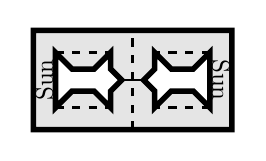
\begin{tikzpicture}
	\begin{scope}[xscale=0.7,yscale=0.7]
	% Draw the Sun Carriage (in this thing to save space)
	
	
	% Try drawing Sun Carriage without rects specifically
	\draw[color=\OutlineColor,fill=\FillColor,even odd rule,line width=\OutlineWidth] 
		(-\SunCarriageWidth,0) rectangle (\SunCarriageWidth,\SunCarriageHeight) % Outer outline
		% Left hole
		(-\SunCarriageWidth+\SunCarriageInternalWidth,\SunCarriageInternalWidth) % bottom left corner
			-- (-\SunCarriageWidth+\SunCarriageInternalWidth,\SunCarriageHeight-\SunCarriageInternalWidth) % top left corner
			-- (-\SunCarriageWidth+\SunCarriageInternalWidth+\SunCarriageFlapWidth,\SunCarriageHeight-\SunCarriageInternalWidth-\SunCarriageFlapWidth) % top flap left vertex
			-- (-\SunCarriageInternalWidth-\SunCarriageFlapWidth,\SunCarriageHeight-\SunCarriageInternalWidth-\SunCarriageFlapWidth) % top flap right vertex
			-- (-\SunCarriageInternalWidth,\SunCarriageHeight-\SunCarriageInternalWidth) % top right corner
			-- (-\SunCarriageInternalWidth,\SunCarriageHeight/2+\SunCarriageIndicatorSize) % right-top
			-- (-\SunCarriageInternalWidth+\SunCarriageIndicatorSize,\SunCarriageHeight/2) % right-point
			-- (-\SunCarriageInternalWidth,\SunCarriageHeight/2-\SunCarriageIndicatorSize) % right-bot
			-- (-\SunCarriageInternalWidth,\SunCarriageInternalWidth) % bottom right corner
			-- (-\SunCarriageInternalWidth-\SunCarriageFlapWidth,\SunCarriageInternalWidth+\SunCarriageFlapWidth) % bottom flap right vertex
			-- (-\SunCarriageWidth+\SunCarriageInternalWidth+\SunCarriageFlapWidth,\SunCarriageInternalWidth+\SunCarriageFlapWidth) % bottom flap left vertex
			-- (-\SunCarriageWidth+\SunCarriageInternalWidth,\SunCarriageInternalWidth) % bottom
			-- cycle
		% Right hole
		(\SunCarriageWidth-\SunCarriageInternalWidth,\SunCarriageInternalWidth) % bottom right corner
			-- (\SunCarriageWidth-\SunCarriageInternalWidth,\SunCarriageHeight-\SunCarriageInternalWidth) % top right corner
			-- (\SunCarriageWidth-\SunCarriageInternalWidth-\SunCarriageFlapWidth,\SunCarriageHeight-\SunCarriageInternalWidth-\SunCarriageFlapWidth) % top flap right vertex
			-- (\SunCarriageInternalWidth+\SunCarriageFlapWidth,\SunCarriageHeight-\SunCarriageInternalWidth-\SunCarriageFlapWidth) % top flap left vertex
			-- (\SunCarriageInternalWidth,\SunCarriageHeight-\SunCarriageInternalWidth) % top left corner
			-- (\SunCarriageInternalWidth,\SunCarriageHeight/2+\SunCarriageIndicatorSize) % left-top
			-- (\SunCarriageInternalWidth-\SunCarriageIndicatorSize,\SunCarriageHeight/2) % left-point
			-- (\SunCarriageInternalWidth,\SunCarriageHeight/2-\SunCarriageIndicatorSize) % left-bot
			-- (\SunCarriageInternalWidth,\SunCarriageInternalWidth) % bottom left corner
			-- (\SunCarriageInternalWidth+\SunCarriageFlapWidth,\SunCarriageInternalWidth+\SunCarriageFlapWidth) % bottom flap left vertex
			-- (\SunCarriageWidth-\SunCarriageInternalWidth-\SunCarriageFlapWidth,\SunCarriageInternalWidth+\SunCarriageFlapWidth) % bottom flap right vertex
			-- (\SunCarriageWidth-\SunCarriageInternalWidth,\SunCarriageInternalWidth) % bottom
			-- cycle; 
		
	% Folding lines
	% Center line
	\draw[\mountainFold,line width=1pt]
		(0,0) -- (0,\SunCarriageHeight);
	% Flap folds
	\draw[\mountainFold,line width=1pt]
		(-\SunCarriageWidth+\SunCarriageInternalWidth,\SunCarriageHeight-\SunCarriageInternalWidth) -- (-\SunCarriageInternalWidth,\SunCarriageHeight-\SunCarriageInternalWidth); % left cell top flap
	\draw[\mountainFold,line width=1pt]
		(-\SunCarriageWidth+\SunCarriageInternalWidth,\SunCarriageInternalWidth) -- (-\SunCarriageInternalWidth,\SunCarriageInternalWidth); % left cell bottom flap
	\draw[\mountainFold,line width=1pt]
		(\SunCarriageWidth-\SunCarriageInternalWidth,\SunCarriageHeight-\SunCarriageInternalWidth) -- (\SunCarriageInternalWidth,\SunCarriageHeight-\SunCarriageInternalWidth); % right cell top flap
	\draw[\mountainFold,line width=1pt]
		(\SunCarriageWidth-\SunCarriageInternalWidth,\SunCarriageInternalWidth) -- (\SunCarriageInternalWidth,\SunCarriageInternalWidth); % right cell bottom flap
		
	% Labels
	\node[scale=0.9,font=\normalsize,rotate=90] at (-\SunCarriageWidth+\SunCarriageInternalWidth/2,\SunCarriageHeight/2) {Sun};
	\node[scale=0.9,font=\normalsize,rotate=-90] at (\SunCarriageWidth-\SunCarriageInternalWidth/2,\SunCarriageHeight/2) {Sun};
		
	% Indicator lines
%	\draw[line width=1pt]
%		(-\SunCarriageInternalWidth,\SunCarriageHeight/2) -- (\SunCarriageInternalWidth,\SunCarriageHeight/2);
	\draw[line width=1pt]
		(-\SunCarriageInternalWidth+\SunCarriageIndicatorSize,\SunCarriageHeight/2) -- (\SunCarriageInternalWidth-\SunCarriageIndicatorSize,\SunCarriageHeight/2);
	
	
%	\draw[fill=\FillColor,even odd rule,line width=\OutlineWidth] 
%		(-\SunCarriageWidth,0) rectangle (\SunCarriageWidth,\SunCarriageHeight)
%		(-\SunCarriageWidth+\SunCarriageInternalWidth,\SunCarriageInternalWidth) rectangle (-\SunCarriageInternalWidth,\SunCarriageWidth-\SunCarriageInternalWidth)
%		(\SunCarriageInternalWidth,\SunCarriageInternalWidth) rectangle (\SunCarriageWidth-\SunCarriageInternalWidth,\SunCarriageWidth-\SunCarriageInternalWidth);
%	% Folding line
%	\draw[dashed,line width=1pt]
%		(0,0) -- (0,\SunCarriageHeight);
%	% Indicator lines
%	\draw[line width=1pt]
%		(-\SunCarriageInternalWidth,\SunCarriageHeight/2) -- (\SunCarriageInternalWidth,\SunCarriageHeight/2);
%%	\draw[line width=1pt]
%%		(-\SunCarriageWidth,\SunCarriageHeight/2) -- (-\SunCarriageWidth+\SunCarriageInternalWidth,\SunCarriageHeight/2);
%%	\draw[line width=1pt]
%%		(\SunCarriageWidth,\SunCarriageHeight/2) -- (\SunCarriageWidth-\SunCarriageInternalWidth,\SunCarriageHeight/2);
%	% Dashed lines for cutting
%	\draw[dotted,line width=1pt]
%		(-\SunCarriageWidth+\SunCarriageInternalWidth,\SunCarriageInternalWidth) -- (-\SunCarriageInternalWidth,\SunCarriageHeight-\SunCarriageInternalWidth);
%	\draw[dotted,line width=1pt]
%		(-\SunCarriageWidth+\SunCarriageInternalWidth,\SunCarriageHeight-\SunCarriageInternalWidth) -- (-\SunCarriageInternalWidth,\SunCarriageInternalWidth);
%		
%	\draw[dotted,line width=1pt]
%		(\SunCarriageWidth-\SunCarriageInternalWidth,\SunCarriageInternalWidth) -- (\SunCarriageInternalWidth,\SunCarriageHeight-\SunCarriageInternalWidth);
%	\draw[dotted,line width=1pt]
%		(\SunCarriageWidth-\SunCarriageInternalWidth,\SunCarriageHeight-\SunCarriageInternalWidth) -- (\SunCarriageInternalWidth,\SunCarriageInternalWidth);
		
	\end{scope}
	\end{tikzpicture}
	\end{center}
	%Then, you can lift each triangular flap and cut it out separately. Alternatively, you may use a hole punch using the marks shown to approximately cut out the interior. Once the interior regions are removed, you can carefully cut out the outer rectangular shape. 
	On the side marked ``Sun'', fold the interior flaps backward. Later, these flaps will help keep this part from sliding along the Solar Arm by providing friction. 
	
	
	% ------------------------------------------------------------------------- %
	\section{Incisions}
	Make an incision along the thick lines on the Observer's Horizon and Time Dial. For the Horizon Disk, this is from the center to due south. For the Time Dial, this is from the center to the zero or 24-hour position. Next, make three incisions on the Solar Frame along the three thick, dark lines: one from the bottom (near its feet), one below ``Time of day $\downarrow$'', and the other above the $80^\circ$N latitude line. Finally, make the two indicated incisions on the Base Support. If printed on cardstock, make the cuts \emph{slightly} wider to accommodate the thickness of the paper. %(Do not make the cuts too wide at first: they can be widened later.)
	
	
	% ------------------------------------------------------------------------- %
	\section{Folds}
	The different dotted/dashed lines have the following meanings: 
	\begin{itemize}
		\item Dotted $\rightarrow$ valley fold (the printed dotted line is in the inside of the fold)
		\item Dashed $\rightarrow$ mountain fold (the printed dashed line is in the outside of the fold)
		\item Dashed and dotted $\rightarrow$ fold both ways (it will need to go both ways)
	\end{itemize}
	
	%For both the frame and the base support: fold the right foot forward (a valley fold) and the left foot back (a mountain fold) along the dashed lines. 
	
	%For the solar indicator box (the smallest piece): carefully fold in half along the dashed line (a mountain fold). 
	
	%For the largest piece, do a mountain fold along the horizontal 
	
	% ------------------------------------------------------------------------- %
	\section{Assembly}
	\subsection{Horizon Disk}
	Temporarily un-fold the center two folds in the Solar Frame (largest piece) and flip it over. Slip the Horizon Disk's incision into the incision in the middle of the Solar Frame such that the support flaps in the middle of the Solar Frame are on top of the Horizon Disk and the degree markings on the Horizon Disk are face-down. Line up the ``Attach here'' bits on the support flap and Horizon Disk, then affix the support flaps using tape. Rotate the horizon disk so that its ``south'' incision slides along the ``Observer's Latitude'' track. It should be loose enough to move easily but tight enough to hold its position when left untouched.
	
	\subsection{Sun Slider}
	Place the folded Sun Slider onto the frame near the solar declination label, such that half of the slider is in front of the Solar Arm and half is behind it. Then, use a small piece of tape to make the Sun Slider into a sleeve around the Solar Arm. (Be careful not to tape the sleeve to the arm!) The slider should be able to slide to different solar declination values. It should be a snug fit: loose enough that your hand can move it, but tight enough that it stays put when you are not touching it. 
	
	\subsection{Base Support}
	Slip the incision furthest from the folds on the base support onto the bottom of the frame, near the folds. The folded feet will be arranged in a windmill pattern for support. If done correctly, six of each letter (A, B, C and D) will be grouped together. Strongly recommended: for added stability, you can tape the feet onto the nearby legs. 
	
	\subsection{Time Dial}
	Slip the Time Dial onto the neck of the Solar Frame. The slit in the Time Dial should line up with the slit on the Solar Frame pointed to by the ``Time of day $\downarrow$'' indicator, and the printed side should be facing up. 
	
	
	% ------------------------------------------------------------------------- %
	\section{How to Use}
	\subsection{Adjust the Viewing Latitude}
	The latitude of the observer can be adjusted by rotating the Observer's Horizon. The southern edge of the horizon disk will point to the observer's latitude on the ``Observer's Latitude'' track. 
	
	\subsection{Adjusting the Time of Year}
	At different times of the year, Earth's tilt causes the Sun to appear more north or more south of the celestial equator (0{\degree} declination). Move the Sun slider to the appropriate declination for the desired date. The solar declination is approximately +23.5{\degree} on/near June~20--21, -23.5{\degree} on/near December~21, and 0{\degree} at either equinox (March~19--20 or September~22--23). 
	
	\subsection{Adjusting the Time of Day}
	The Solar Arm (labelled ``Solar Declination'') acts like a hinge. Its position indicates the rotation of the Earth --- or equivalently, the time of day. The Solar Arm has an indicator at the bottom which points to the time of day on the time dial. For example, at 6~AM the Solar Arm will be aligned with E (east) on the horizon disk and 6 on the Time Dial. 
	
	\subsection{Simulating the Sun's Daily Motion}
	You can simulate the position of the Sun in the sky by pivoting the Solar Arm from 0 (midnight) to 6 (6~AM) to 12 (noon) to 18 (6~PM) to 24 (midnight). The Sun slider represents the Sun. Sunrise happens when the Sun slider crosses from behind the horizon disk (usually in the eastern sky) in the morning. Sunset happens when the Sun slider crosses from above the horizon disk to below it (usually in the western sky) in the evening. Some people find it helpful to rotate the entire model such that the printed Horizon Disk faces up.
\vfill
\hrule 
%\noindent\copyright 2025 by \href{https://www.lpl.arizona.edu/~vriesema/}{Jess W. Vriesema} of Calvin University. All rights reserved. 
	\end{multicols}
\fi % \ifPrintInstructions







% ------------------------------------------------------------------------- %
% Wishlist (To Do List)
% ------------------------------------------------------------------------- %

\ifPrintWishlist
	\newpage
	\newgeometry{letterpaper,margin=0.5cm}
	
	\section*{To Do List}
	The following are things that should be done when I have time. Chores. 
	\begin{itemize}
		\item Add dates to Solar Arm? (Maybe at bottom?) Make switch for this so educators can decide how many clues to give students.
		\item Add compass markings for solar declination beyond the Sun's extent, but highlight the real ones?
		\item Add ``Observer's Latitude'' indicator arrow on the Horizon Disk, as with the Time Disk and Solar Arm. 
		\item Make a version with AM/PM times instead of 24-hour time. Adjust instructions accordingly. 
		\item Make a switch to use the Solar Carriage flaps (else just a box)
		\item Revise the instruction card and instructions to use less jingo. 
		\item Clarify the license terms somewhere?
		\item Move the ``S'' off-axis somewhat, since it gets sliced in two otherwise?
		\item Draw cardinal points on the back of the horizon disk? 
		\item The angles in the Solar Frame need some adjustment. Note the pgfsetmacro commands to account for the outline width thickness and such. The stuff in the asin() functions is only approximate right now. That needs to be done for the laser cut things, too. 
		\item Make the horizon disk's support flap have a shape that has a unique orientation. 
		\item Typeset the URLs better: href vs. url?
		\item Adjust the ``Base Support'' and ``Solar Frame'' labels and their kin. 
		\item Improve instructions:
		\begin{itemize}
			\item Update instructions for how the horizon disk should be when taped onto the solar frame. This was frustrating for me (the designer!) this past time. 
			\item Organize better? 
			\item Add introduction? 
			\item Add space to the instruction card to affix the base?
		\end{itemize}
	\end{itemize}


	\section*{Wishlist}
	The following are things I'd love to do when I have some creative inspiration. Non-necessary. 
	\begin{itemize}
		\item Figure out a way to attach the base support and solar frame without tape (e.g. inserting a paper slip into a slit). 
		\item Give friction to sliders
		\begin{itemize}
			\item Make the central latitude angle indicator and Solar Arm (near Solar Slider) edge be more of a small-scale (0.5mm?) square wave --- at least when laser cutting. Then, students could fold the tiny flaps in or out, which would provide some friction against whatever was sliding.
		\end{itemize}
		\item Make a more advanced version for advanced students:
		\begin{itemize}
			\item Discuss the \href{https://en.wikipedia.org/wiki/Analemma}{analemma} or \href{https://en.wikipedia.org/wiki/Equation_of_time}{Equation of Time}?
			\begin{itemize}
				\item Add a mini analemma to the solar arm to show dates? (If so, I might need to thicken the solar arm in order to fit the text in there.)
			\end{itemize}
			\item Adjust to calculate earliest/latest sunset times, WHICH ARE NOT SOLSTICES. See ``\href{https://en.wikipedia.org/wiki/Analemma#Earliest_and_latest_sunrise_and_sunset}{Earliest and latest sunrise and sunset}'' for info. 
		\end{itemize}
		\item Make good use of the backside of the instruction card? 
		\begin{itemize}
			\item Add a diagram or pic of the finished product?
			\item Add brief assembly instructions?
			\item Add a QR code for downloading this thing? 
			\item Determine a clever way to put a copyright symbol on the printed material somewhere. 
		\end{itemize}
		\item Have a star in or outside of the Solar Carriage?
		\item Determine the best way to perforate folds with laser cutter: 
		\begin{itemize}
			\item What is an ideal perforation: dashed? dotted? solid line through middle?
		\end{itemize}
		\item Create an activity or two to go with this: 
		\begin{itemize}
			\item One version for younger students, one for university students?
			\item Things to include (following \href{https://cft.vanderbilt.edu/guides-sub-pages/blooms-taxonomy/}{Revised Bloom's Taxonomy}): 
			\begin{itemize}
				\item Remember / Recall (understand how to use the model by recalling directions)
				\begin{itemize}
%					\item Where is the Sun at noon: north, south, east or west? 
					\item What does moving the ``Solar Arm'' simulate?
					\item How can you change the observer's latitude? 
					\item How can you change the time of day? 
					\item How can you change the time of year? 
				\end{itemize}
				\item Understand / Explain
				\begin{itemize}
					\item If the Horizon Disk is rotated such that ``N'' is at the top and ``S'' is toward the base, what latitude does this correspond to? 
				\end{itemize}
				\item Apply / Use Information
				\begin{itemize}
					\item Find a date when the Sun is highest/lowest in the sky at your latitude.
					\item Does the Sun always rise in the east and set in the west? 
					\item What time does the Sun rise and set today at your latitude?
					\item What time of year is the Sun the highest/lowest in the sky at your latitude?
					\item What time is the Sun highest in the sky? 
					\item What time of year has the longest/shortest length of day at your latitude?
					\item Find a latitude and time of year such that the Sun never sets or rises.
					\item Find a latitude at which the Sun is directly overhead on a given date.
					\item Predict/calculate sunrise times as a function of latitude and time of day. 
				\end{itemize}
				\item Analyze / Draw Connections
				\begin{itemize}
					\item How does the sunrise/sunset \emph{time} change with the time of year? 
					\item How does the length of day change with the time of year? 
					\item How does the sunrise/sunset \emph{location} change with the time of year? 
					\item How does the length of day change with the time of year? 
					\item Is the Sun highest in the sky at the same location (azimuth) for different times of the year? {\color{red}{(Reword)}}
					\item Predict/calculate critical latitudes (arctic/antarctic circles, tropics).
				\end{itemize}
				\item Evaluate
				\begin{itemize}
					\item This model works if the time is understood as local solar time. How would this model change depending on a person's east/west location within their timezone?
					\item What are some limitations of this model? % Not accurate for discrete timezones, does not model topography, doesn't account for the ellipticity of Earth's orbit, ...
					\item This model does not account for the \href{https://en.wikipedia.org/wiki/Analemma}{analemma}. What differences are there in this model? 
				\end{itemize}
				\item Create
				\begin{itemize}
					\item Based on this model, explain how the Sun causes the seasons. 
					\item Use this model to explain what would be different if the Earth were tilted at $40^\circ$ instead of $23.5^\circ$ (solar motions, seasons, temperatures, etc.). 
				\end{itemize}
				
			\end{itemize}
		\end{itemize}
	\end{itemize}

\fi %  \ifPrintWishlist

%}%  end of resizebox
%}%  end of resizebox
\end{document}
